\RequirePackage{lineno}
%\documentclass[preprint,superscriptaddress,nofootinbib, notitlepage, double-spaced, showpacs,floatfix,longbibliography]{revtex4-1}
\documentclass[review]{elsarticle}
%\documentclass[twoside,12pt]{article}
%\linenumbers
\usepackage{verbatim}
\usepackage{graphicx}
\usepackage[utf8]{inputenc}
\usepackage[usenames,dvipsnames,svgnames,table]{xcolor}
\usepackage[breaklinks=true,colorlinks=true,linkcolor=blue,urlcolor=blue,citecolor=blue]{hyperref}
\usepackage{rotating}
\usepackage{graphicx}% Include  files
\usepackage{dcolumn}% Align table columns on decimal point
\usepackage{bm}% bold math
\usepackage{epsfig}
\usepackage{hyperref}
\usepackage{ulem}
\usepackage{appendix}
%\usepackage{iopams}
\usepackage{mwe}
\usepackage{subfig}
\usepackage{lineno}
\expandafter\let\csname equation*\endcsname\relax
\expandafter\let\csname endequation*\endcsname\relax
\usepackage{amsmath}
\usepackage{geometry}
\newgeometry{vmargin={20mm}, hmargin={30mm,22mm}}
%Uncomment next line if AMS fonts required
\usepackage{times}  
%% `Elsevier LaTeX' style
\bibliographystyle{elsarticle-num}
%\usepackage[backend=biber,style=nature]{biblatex}
%\addbibresource{BeautyExp.bib}

%%%% new commands
\newcommand{\barb}{{\bar{b}}}
\newcommand{\barc}{{\bar{c}}}
\newcommand{\SNN}{$\sqrt{s_{NN}}=$ }
\newcommand{\sqrtsnn}{\ensuremath{\sqrt{s_{NN}}}\xspace}
\newcommand{\raa}{$R_{AA}~$}
\newcommand{\pt}{$p_{T}$}
\newcommand{\npart}{$N_{\rm Part}~$}
\newcommand{\Jpsi}{\ensuremath{J\hspace{-.08em}/\hspace{-.14em}\psi}\xspace} % J/Psi (no mass)
\newcommand{\qqbar}{\ensuremath{q \overline{q}\xspace}\xspace}
\newcommand{\QQbar}{\ensuremath{Q \overline{Q}\xspace}\xspace}
\newcommand{\pp}{{\ensuremath{pp}}\xspace}
\newcommand{\PgU}{\ensuremath{\Upsilon}\xspace}
\newcommand{\PgUa}{\ensuremath{\Upsilon\text{(1S)}}\xspace}
\newcommand{\PgUb}{\ensuremath{\Upsilon\text{(2S)}}\xspace}
\newcommand{\PgUc}{\ensuremath{\Upsilon\text{(3S)}}\xspace}
\newcommand{\fig}[1]{Fig.~\ref{#1}\xspace}
\newcommand{\tab}[1]{Tab.~\ref{#1}\xspace}
\newcommand{\pT}{p_{T}}
\newcommand{\sNN}{\sqrt{s_{_{NN}}}}


\newcommand{\jpsi}{\ensuremath{\mathrm{J}/\psi}\hspace {0.05in}} 
\newcommand{\ups}{\ensuremath{\Upsilon}\hspace {0.05in}}
\newcommand{\upsa}{\ensuremath{\Upsilon\mathrm{(1S)}}\hspace {0.05in}}
\newcommand{\upsb}{\ensuremath{\Upsilon\mathrm{(2S)}}\hspace {0.05in}}
\newcommand{\upsc}{\ensuremath{\Upsilon\mathrm{(3S)}}\hspace {0.05in}}
\newcommand{\upsbc}{\ensuremath{\Upsilon\mathrm{(2S+3S)}}\xspace}
\newcommand{\upsabc}{\ensuremath{\Upsilon\mathrm{(1S+2S+3S)}}\xspace}
\newcommand{\upsn}{\ensuremath{\Upsilon\mathrm{(nS)}}\xspace}
\newcommand{\doubleRatioUps}{\ensuremath{\left.(N_{\upsb}/N_{\upsa})_{\mathrm{Pb-Pb}}/(N_{\upsb}/N_{\upsa})_{\mathrm{pp}}\right.\xspace}}
\newcommand{\psiP}{\ensuremath{\psi\mathrm{(2S)}}\hspace {0.05in}}
\newcommand{\chic}{\ensuremath{\chi_c}\hspace {0.05in}}
\newcommand{\chib}{\ensuremath{\chi_b}\hspace {0.05in}}



\newcommand{\Qcal}{\ensuremath{\Phi\xspace}}
\newcommand{\ccbar}{\ensuremath{{c\overline{c}}}\xspace}
\newcommand{\bbbar}{\ensuremath{{b\overline{b}}}\xspace}

\newcommand{\sqrts}{\ensuremath {\sqrt{s}}\hspace {0.05in}}

\newcommand{\be}{\begin{equation}}
\newcommand{\ee}{\end{equation}}
\newcommand{\bea}{\begin{eqnarray}}
\newcommand{\eea}{\end{eqnarray}}
\newcommand{\nn}{\nonumber}

\begin{document}
%\begin{frontmatter}
  \title{Production of bottomonia states in proton-proton and heavy ion collisions}
  \author[NPD]{Vineet Kumar}
  \author[NPD,HBNI]{Prashant Shukla}
  \author[UOC]{Abhijit Bhattacharyya\corref{mycorrespondingauthor}}
  \cortext[mycorrespondingauthor]{Corresponding author}
  \ead{abhattacharyyacu@gmail.com}
  \address[NPD]{Nuclear Physics Division, Bhabha Atomic Research Centre, Mumbai 400085, India}
  \address[HBNI]{Homi Bhabha National Institute, Anushakti Nagar, Mumbai 400094, India}
  \address[UOC]{Department of Physics, University of Calcutta, 92, A. P. C. Road Kolkata-700009, India}
  \date{\today}



\fontsize{11}{15}
\selectfont


  
\begin{abstract}
    
 In this work, we review the experimental  and theoretical developments of bottomonia
production in proton-proton and heavy ion collisions. Bottomonia production process
is one of the most robust processes to investigate the fundamental aspects of
Quantum Chromodynamics. The field has been enriched by immense theoretical and 
experimental activities in last few years.
In this write up, emphasis is given to the lessons learnt from the LHC
data, which are reviewed in a global perspective with the results from the RHIC at
lower energies are used
for comparison. The review covers bottomonia production in proton-proton,
proton-nucleus and nucleus-nucleus
collisions and includes discussion both hot and cold effects of
strongly interacting matter.

\end{abstract}
  
  
%\maketitle 

\begin{keyword}
   Beauty, Quarkonium, Bottomonium, Hadron Collision, Heavy-Ion Collision, Quark-Gluon Plasma, LHC, RHIC
\end{keyword}
  

%\vspace{2pc}
%\noindent{\it Keywords}: Beauty, Quarkonium, Hadron Collision, Heavy-Ion Collision, Quark-Gluon Plasma, LHC, RHIC

  

\maketitle

\tableofcontents


%\end{frontmatter}

\newpage
\section{Introduction}
\label{sec:Introduction}


The strong interaction among quarks and gluons is described by
Quantum Chromodynamics (QCD) that has two regimes; asymptotic freedom at short distance
and colour confinement at long distances.
At short distance, the interaction can be well described using perturbative methods. 
However, confinement, which is a non-perturbative phenomenon, is not very well understood till date.    
The study of quarkonia ($Q\bar{Q}$) is a unique tool 
which takes care of  both of these perturbative and non-perturbative aspects of QCD.
An important characteristic of the quarkonia states is the  small velocity, $v$, of the massive
constituents. This feature allows one to   treat these states using non-relativistic formalism~\cite{Povh:1995mua,Ikhdair:2005jf}. 
In a simple picture,  a quarkonium can be thought of as a heavy quark pair ($Q\bar{Q}$) bound
in a colour singlet state by some effective potential interaction.  In this bound state the constituents are 
separated by distances much smaller than $1/\Lambda_{\rm QCD}$ where $\Lambda_{\rm QCD}$
is the QCD scale.
%This interaction gets screened 
%in the presence of a deconfined medium like Quark Gluon Plasma (QGP), causing 
%the bound state to melt away and thus the quarkonia yields are suppressed in the 
%heavy ion collisions. This makes quarkonia an important probe of QGP. However cold nuclear matter 
%effects such as modification of parton distribution functions of nucleons inside nucleus also 
%affect their yields.


It is expected that the dynamics of strongly interacting matter changes
at temperatures and/or densities which are similar to or larger than
the typical hadronic scale.
It has been argued that under such extreme conditions, 
one should have the onset of deconfinement of quarks and gluons  and thus the 
description of strongly-interacting matter could then
be understood in terms of these elementary degrees of freedom.
This new form of matter is known as 
quark-gluon plasma~\cite{Shuryak:1980tp,Satz:2011wf}, or QGP.
The existence of such a transition has indeed been demonstrated 
from first principles using simulations of lattice QCD.
In  heavy-ion collisions~\cite{Satz:2000bn} one can study the deconfinement transition 
and the properties of hot and dense strongly-interacting 
matter. 
Significant parts of different experimental heavy-ion
programmes are dedicated to studying quarkonium yields. Such studies are 
motivated by the suggestion of  Matsui and Satz
that quarkonium suppression could be a signature of 
deconfinement~\cite{Matsui:1986dk}.
In fact, the observation of anomalous suppression was proposed to be
a key signature of deconfinement at SPS energies~\cite{Kluberg:2005yh}.




The $\Upsilon^{'}$s having three states with different binding
energies are far richer probes of the QCD dynamics in p+p and Pb+Pb collisions than
the charmonia.
It is therefore important to achieve a good understanding of their
production mechanism in the vacuum as well as of how the nuclear effects in proton-nucleus
collisions affect them.
  At Large Hadron Collider (LHC) energy, the cross section of bottomonia production is large and
also the detector technologies enabled the study of various bottomonia 
states separately both in p+p and heavy ion collisions.
As proposed by different theories, bottomonium is an important and clean probe 
of hadronic collisions for at least two reasons. 
First, the effective field theory approach, which provides a link to first 
principles QCD, is more suitable for bottomonium due to better separation of 
scales and higher binding energies. Second, the statistical recombination effects 
are less important due to  the heavier bottom quarks.  
Experimentally, there is a smaller background contribution in bottomonium
mass region and its decay in dimuon channel provides a reconstruction with better
mass resolution. 
 All these properties make bottomonium a good probe of 
QGP formation in heavy ion collisions.


There have been immense
experimental~\cite{Sirunyan:2017isk,Sirunyan:2017lzi,CMS:2018zza,Acharya:2019iur,ALICE:2018wzm}
and theoretical works~\cite{Strickland:2011mw,Song:2011nu,Kumar:2014kfa,Kumar:2019xdj} on
quarkonia modifications in Pb+Pb collisions.
The botomonia states in heavy ion collisions are suppressed with respect to their yields
in proton-proton collisions scaled by the number of binary nucleon-nucleon
(NN) collisions.
The amount of quarkonia suppression is expected to be sequentially ordered by the binding
energies of the quarkonia states.
 As the screening depends on the  binding energy the bottomonium states ($\Upsilon$(1S), $\Upsilon$(2S),
$\Upsilon$(3S), $\chi_{b}$, etc.) are extremely useful probes to understand the color screening
properties of the QGP.
The sequential suppression of the yields of $\Upsilon$(nS) states was first observed by
CMS at $\sNN =$2.76 TeV~\cite{Chatrchyan:2011pe,Chatrchyan:2012lxa}. More recently, results with improved
statistical precision have been reported by both the ALICE~\cite{ALICE:2018wzm}
and CMS Collaborations ~\cite{Sirunyan:2017lzi,CMS:2018zza} at $\sNN =$5.02 TeV.
The suppression of the $\Upsilon$(1S)
meson has also been studied at $\sNN =$200 GeV at Relativistic Heavy Ion Collider (RHIC)~\cite{STAR:2013kwk}, although the
bottomonia production cross section is small at lower energies. 

In this writeup, we review experimental and theoretical aspects of bottomonia production in p+p, p+A
and A+A collisions at RHIC and LHC energies.









\section{Bottomonia production p-p collisions: Experimental overview}

{\color{red}
  Here all description of measured data of bottomonium should come.
  Take from NRQCD paper} 

Heavy-flavour production in pp collisions provides important tests of our understanding of various aspects of QCD.
The heavy-quark mass acts as a long distance cut-off so that the partonic hard-scattering process can be calculated
in the framework of perturbative QCD down to low transverse momenta. When the heavy-quark pair forms a quarkonium bound
state, this process is non-perturbative as it involves long distances and soft momentum scales. Therefore, the detailed
study of heavy-flavour production and the comparison to experimental data provides an important testing ground for
both perturbative and non-perturbative aspects of QCD calculations.

%% Upsilon discovery

The $\Upsilon$ meson was discovered by E288 collaboration at Fermilab in 400 GeV proton nucleus
collisions in 1977~\cite{PhysRevLett.39.252}.
%%Upsilon measurements at Tevatron
The Collider Detector at Fermilab (CDF) reports $\Upsilon$(1S), $\Upsilon$(2S) and $\Upsilon$(3S) 
differential (d$^{2}\sigma$/dp$_{T}$dy) and integrated cross sections in p$\overline{\rm p}$ collisions at
$\surd$s = 1.8 TeV~\cite{CDF:1995gwi}. The three resonances were reconstructed through the decay of
$\Upsilon$(nS) to $\mu^{+}$ and $\mu^{-}$. The differential (d$^{2}\sigma$/dp$_{T}$dy) and integrated
cross sections have measured in the range 0$\textless$p$_{T}\textless$16 GeV/c for $\Upsilon$(1S) and in the range
0$\textless$p$_{T}\textless$10 GeV/c for $\Upsilon$(2S) and $\Upsilon$(3S). Table~\ref{Tab:YCrossCDF95} summarizes
the 1995 CDF Run I cross section measurement~\cite{CDF:1995gwi}.    

\begin{table}
  \begin{center}
    \caption[]{CDF Run I $\Upsilon$ cross section measurement with luminosity of 16.6 pb$^{-1}$ with $|y|\textless$ 0.4 at
    $\surd$s = 1.8 TeV.}
\label{Tab:YCrossCDF95}
\begin{tabular}{cc} 
\hline 
\hline
$\Upsilon$(nS) state             &$\frac{d\sigma(\Upsilon(nS))}{dy}\times B(\Upsilon(nS)\rightarrow\mu^{+}\mu^{-})$ (pb)    \\              
\hline
$\Upsilon$(1S)                   &753$\pm$29(stat.)$\pm$72(syst.)\\
$\Upsilon$(2S)                   &183$\pm$18(stat.)$\pm$24(syst.)\\
$\Upsilon$(3S)                   &101$\pm$15(stat.)$\pm$13(syst.)\\   
\hline
\hline
\end{tabular}
\end{center}
\end{table}

In 2002, CDF Run I measured both the $\Upsilon$ cross section and polarization with
an integrated luminosity of 77 pb$^{-1}$~\cite{CDF:2001fdy}. The cross section results from the CDF
Run I measurement from 2002 are listed in Table~\ref{Tab:YCrossCDF02}.


\begin{table}
  \begin{center}
    \caption[]{CDF Run I $\Upsilon$ cross section measurement with luminosity of 77.0 pb$^{-1}$ with $|y|\textless$ 0.4 at
    $\surd$s = 1.8 TeV.}
\label{Tab:YCrossCDF02}
\begin{tabular}{cc} 
\hline 
\hline
$\Upsilon$(nS) state             &$\frac{d\sigma(\Upsilon(nS))}{dy}\times B(\Upsilon(nS)\rightarrow\mu^{+}\mu^{-})$ (pb)    \\              
\hline
$\Upsilon$(1S)                   &680$\pm$15(stat.)$\pm$18(syst.)$\pm$26(lumi.)\\
$\Upsilon$(2S)                   &175$\pm$9(stat.)$\pm$8(syst.)\\
$\Upsilon$(3S)                   &97$\pm$8(stat.)$\pm$5(syst.)\\   
\hline
\hline
\end{tabular}
\end{center}
\end{table}







%%Upsilon measurements at RHIC



%%Upsilon at LHC
The study of bottomonium production at LHC energies offers many advantages. First, there is no beauty feed-down. Second,
owing to their larger masses, their decay products - usually leptons - are more energetic and more easily detectable
(detector acceptance, trigger bandwidth, etc.). Third, the existence of three sets of bottomonia with their principal
quantum number n = 1, 2, 3 below the open-beauty threshold offers a wider variety of states that can be detected in
the dilepton decay channel this, however, introduces a complicated feed-down pattern.



With the advent of the LHC, the study of $\Upsilon$ production has become more
accessible than ever. The $\Upsilon$ production pattern at the LHC differs from that
of the lighter $\psi^{'}$s. The $\Upsilon^{'}$s having three states with different binding
energies are thus far richer probes of the QCD dynamics in pp and PbPb collisions than
the charmonia. It is therefore important to achieve a good understanding of their
production mechanism in the vacuum as well as of how the nuclear effects in proton-nucleus
collisions affect them. In this section we will give an overview of measurements of $\Upsilon$
production in pp collisions at LHC. 

The measurements of $\Upsilon$(1S,2S,3S) production in pp collisions at the unprecedented C.M. energies
of 2.76, 5.02, 7, 8, and 13 TeV have been undertaken, within the rapidity window -2.4$<$ y $<$ 4.5
and the dimuon momentum range of p$_{T}<$ 100 GeV/c at LHC by ALICE~\cite{ATLAS:2011nal,ATLAS:2012lmu}, ATLAS~\cite{ATLAS:2011nal,ATLAS:2012lmu},
CMS~\cite{CMS:2013qur,CMS:2017dju} and LHCb collaborations.

In addition, the angular distribution of the muons produced in the $\Upsilon$(1S, 2S, 3S) decays has
been analyzed in different reference frames to determine the polarization parameters. From the results
of CMS and LHCb, $\Upsilon$(1S, 2S, 3S) polarization parameters are all so close to zero that polarizations
can be neglected. The measurements of these cross sections and polarizations have shed light on the
$\Upsilon$(1S, 2S, 3S) production mechanisms in pp collisions.
Analysis of new LHC data will extend the reach of the kinematics to test the NRQCD with
higher-order corrections which becomes more sensitive with the increase of p$_{T}$,












\section{Bottomonia production mechanism in p-p collisions}
\label{sec:Bottomonia_pp_th}


In general one can subdivide the quarkonia production process into two major parts

\begin{enumerate}
\item Production of a heavy quark pair in hard collisions.
\item Formation of quarkonia out of the two heavy quarks.
\end{enumerate}


The massive quarks (with $m_c\sim 1.6$ GeV/$c^2$, $m_b\sim 4.5$ GeV/$c^2$) are produced
in initial stages in hadronic collision with high momentum transfer and thus
can be treated perturbatively~\cite{Nason:1989zy}. The emergence of quarkonia
out of the two massive quarks, on the other hand can only be described non-perturbatively using different
models~\cite{Bodwin:1994jh,Brambilla:2014jmp}.
The Colour Singlet Model (CSM)~\cite{Einhorn:1975ua,Berger:1980ni},
Colour Evaporation Model (CEM)~\cite{Fritzsch:1977ay,Amundson:1995em}, the Fragmentation Scheme and 
the NRQCD factorisation formalism are some of the well established models for quarkonia production.


Due to the high mass of the heavy quarks they are produced in the initial
collisions as their production requires sufficiently high momentum 
transfers. For this reason the heavy quark production
is a hard process that can be treated perturbatively.
The hadronic cross section in $pp$ collisions can
be written as
\begin{eqnarray}
\sigma_{pp}(s,m^2) & = & \sum_{i,j = q, \overline q, g} 
\int dx_1 \, dx_2 \, 
f_i^p (x_1,\mu_F^2) \,
f_j^p(x_2,\mu_F^2) \, \widehat{\sigma}_{ij}(s,m^2,\mu_F^2,\mu_R^2)
\label{sigpp}
\end{eqnarray}
where $x_1$ and $x_2$ are the fractional momenta carried by the colliding
partons and $f_i^p$ are the proton parton densities.
The total partonic cross section has been completely calculated up to NLO
\cite{Nason:1987xz,Nason:1989zy}. The partonic cross section is given by
\begin{eqnarray}
\widehat{\sigma}_{ij}(s,m,\mu_F^2,\mu_R^2) & = & 
\frac{\alpha_s^2(\mu_R^2)}{m^2}
\left\{ f^{(0,0)}_{ij}(\rho) \right. \nonumber \\
 & + & \left. 4\pi \alpha_s(\mu_R^2) \left[f^{(1,0)}_{ij}(\rho) + 
f^{(1,1)}_{ij}(\rho)\ln\bigg(\frac{\mu_F^2}{m^2} \bigg) \right] 
+ {\cal O}(\alpha_s^2) \right\}
\,\, 
\label{sigpart}
\end{eqnarray}
where $\rho = 4m^2/s$ and 
$f_{ij}^{(k,l)}$ are the scaling functions to NLO \cite{Nason:1987xz,Nason:1989zy}. 
At small $\rho$, the ${\cal O}(\alpha_s^2)$ and ${\cal O}(\alpha_s^3)$
$q \overline q$ and the ${\cal O}(\alpha_s^2)$ $gg$ scaling functions 
become small while the ${\cal O}(\alpha_s^3)$ $gg$ and $qg$ scaling functions
plateau at finite values.  Thus, at collider energies, the total cross sections
are primarily dependent on the small $x$ parton densities and phase space.
The total cross section does not depend on any kinematic variables, 
only on the quark mass, $m$, and the renormalization and factorization scales with central
value $\mu_{R,F} =\mu_0 = m$.


The nonperturbative evolution of the $Q\bar Q$ pair into a quarkonium
has been discussed extensively in terms of models and in terms of the
language of effective theories of QCD
\cite{Bodwin:1994jh,Brambilla:2004wf}. Different
treatments of this evolution have led to various theoretical models for
inclusive quarkonium production. Most notable among these are the color-singlet
model (CSM), the color-evaporation model (CEM) and the non-relativistic QCD
(NRQCD) factorization approach. In this review we will mainly discuss the NRQCD 
approach, as theoretically, it is the most modern and acceptable one. However,
we will touch upon CSM and CEM briefly. 





\subsection{The color singlet model}


The color singlet model (CSM) was first proposed shortly after the discovery of the 
$\Jpsi$~\cite{Einhorn:1975ua,Ellis:1976fj,Carlson:1976cd,Berger:1980ni}.
In this model, it is assumed that the $Q\bar Q$ pair that evolves into
the quarkonium is in a color-singlet state and that it has the same spin
and angular-momentum quantum numbers as the quarkonium. In the CSM, the
production rate for each quarkonium state is related to the absolute
values of the color-singlet $Q\bar Q$ wave function and its derivatives,
evaluated at zero $Q\bar Q$ separation. These quantities can be
extracted by comparing theoretical expressions for quarkonium decay
rates in the CSM with experimental measurements. Once this extraction
has been carried out, the CSM has no free parameters. The CSM was
successful in predicting quarkonium production rates at relatively low
energy \cite{Schuler:1994hy}. Recently, it has been found that, at high
energies, very large corrections to the CSM appear at next-to-leading
order (NLO) and next-to-next-to-leading order (NNLO) in $\alpha_s$
\cite{Artoisenet:2007xi,Campbell:2007ws,Artoisenet:2008fc}.
Consequently, the possibility that the CSM might embody an important 
production mechanism at high energies has re-emerged. 
However, given the very large corrections at
NLO and NNLO, it is not clear that the perturbative expansion in
$\alpha_s$ is convergent. 
%Furthermore, in the production and decay of
%$P$-wave and higher-orbital-angular-momentum quarkonium states, the CSM
%is known to be inconsistent because it leads to uncanceled infrared
%divergences. (See Ref.~\cite{Brambilla:2004wf} and references therein.)
%The NRQCD factorization approach encompasses
%the color-singlet model, but goes beyond it.

\subsection{The color evaporation model}  
\label{prod_sec:CEM}

The CEM~\cite{Fritzsch:1977ay,Amundson:1995em,Amundson:1996qr}
is motivated by the principle of quark-hadron duality. In the CEM, it
is assumed that every produced $\QQbar$ pair evolves into a quarkonium
if it has an invariant mass that is less than the threshold for
producing a pair of open-flavor heavy mesons. It is further assumed that
the nonperturbative probability for the $\QQbar$ pair to evolve into a
quarkonium state $H$ is given by a constant $F_H$ that is
energy-momentum and process independent. Once $F_H$ has been fixed by
comparison with the measured total cross section for the production of
the quarkonium $H$, the CEM can predict, with no additional free
parameters, the momentum distribution of the quarkonium production rate. The
CEM predictions provide good descriptions of the CDF data for $\Jpsi$,
$\psi(2S)$, and $\chi_{c}$ production at $\sqrt{s}=1.8$~TeV
\cite{Amundson:1996qr}. 

%In Ref.~\cite{Bodwin:2005hm}, the CEM
%predictions are fit to the CDF data for $J/\psi$, $\psi(2S)$, and
%$\chi_{cJ}$ production at $\sqrt{s}=1.8$~TeV \cite{Abe:1997yz}. The
%quality of these fits is generally poor, with $\chi^2/\hbox{d.o.f.}$ for
%the $J/\psi$ fits of about $7$--$8$ without initial-state $k_T$ smearing and
%$2$--$4.5$ with initial-state $k_T$ smearing. In contrast, the NRQCD
%factorization approach, which we are about to describe, yields fits to
%the CDF $J/\psi$ data with $\chi^2/\hbox{d.o.f.}$ of about $1$.

The heavy quark production cross section are calculated to NLO in pQCD  
using the CT10 parton densities \cite{Lai:2010vv}. The mass and scale parameters used 
for open and hidden heavy flavor production are obtained by fitting the energy dependence 
of open heavy flavor production to the measured total cross sections~\cite{Nelson:2012bc}.
%Those obtained for open charm are $m_c = 1.27 \pm 0.09$~GeV,
%$\mu_F/m_{T\,c} = 2.10 ^{+2.55}_{-0.85}$, and $\mu_R/m_{T\, c} = 1.60 ^{+0.11}_{-0.12}$~\cite{Nelson:2012bc}. 
The botttom quark mass and scale parameters are $m_b = 4.65 \pm 0.09$ GeV,
$\mu_F/m_{T\, b} = 1.40^{+0.75}_{-0.47}$, and $\mu_R/m_{T\, b} = 1.10^{+0.26}_{-0.19}$.
The quarkonium production cross sections are calculated in the color evaporation model with
normalizations determined from fitting the scale parameter to the shape of the energy-dependent
cross sections~\cite{Nelson:2012bc}.
% The resulting uncertainty bands are smaller 
%than those obtained with the fiducial parameters used in Ref.~\cite{Cacciari:2005rk}.
%We note that the new results are within the uncertainties of those Ref.~\cite{Cacciari:2005rk}.  
%Indeed, the charm cross sections reported at the LHC agree
%better with the new values of the mass and scale than the central value of $m_c = 1.5$ GeV,
%$\mu_F/m_T = \mu_R/m_T = 1$.
The central EPS09 NLO parameter set~\cite{Eskola:2009uj} is used to 
calculate the modifications of the parton distribution functions (nPDF) in 
Pb+Pb collisions, referred as cold nuclear matter (CNM) effects.
The production cross sections for heavy flavor and quarkonia at $\sqrt{s_{_{_{NN}}}}$ = 2.76 
TeV \cite{Kumar:2012qx} are given in Table~\ref{NLOcros}.  The yields in a minimum bias 
Pb+Pb event is obtained from the per nucleon cross
section, $\sigma_{\rm PbPb}$, in Table~\ref{NLOcros}, as
\begin{eqnarray}
N = {A^2 \sigma_{\rm PbPb} \over  
\sigma_{\rm PbPb}^{\rm tot}} \, \, .
\end{eqnarray}
 At 2.76 TeV, the total Pb+Pb cross section, $\sigma_{\rm PbPb}^{\rm tot}$, 
is 7.65 b \cite{Chatrchyan:2011sx}.


\begin{table}
  \begin{center}
\caption[]{Heavy quark and quarkonia production  cross sections at
$\sqrt{s_{_{_{NN}}}}= 2.76$ TeV. The cross sections are given per nucleon pair while
$N^{\rm PbPb}$ gives the initial number of heavy quark pair/quarkonia per Pb+Pb event.}
\label{NLOcros}
\begin{tabular}{l|l|l|l|l} 
\hline 
\hline
             & $ c \overline c$            &$\Jpsi$                      & $ b \overline b$                    & $\Upsilon$   \\              
\hline
$\sigma_{pp}$ & $4.11^{+2.69}_{-2.50}$ mb    & $21.6^{+10.6}_{-10.4}~\mu$b   & $110.5^{+15.1}_{-14.2}~\mu$b            & $0.22^{+0.07}_{-0.06}~\mu$b  \\


$\sigma_{\rm PbPb}$ & $3.21^{+2.1}_{-1.95}$ mb    &16.83$^{+8.26}_{-8.10}~\mu$b    & $100.5^{+13.7}_{-12.9}~\mu$b             & 0.199$^{+0.063}_{-0.054}~\mu$b  \\



$N^{\rm PbPb}$     & $18.12^{+12}_{-11}$       & $0.0952^{+0.047}_{-0.046}$         & $0.57^{+0.08}_{-0.07}$                          & $0.001123^{+0.0004}_{-0.0003}$       \\

\hline
\hline
\end{tabular}
\end{center}
\end{table}






\subsection{The NRQCD factorization approach}


In the framework of CSM, the $Q\bar{Q}$ pair, eventually evolving into the quarkonium,
is assumed to be in Colour Singlet (CS) state and that has spin and 
angular momentum same as that of quarkonium.
Apart from comprising of the CSM, the NRQCD factorisation approach incorporates 
the Colour Octet (CO) states as well.

In the formalism of the NRQCD factorisation approach, the evolution probability of $Q\bar{Q}$
pair into a state of quarkonium is expressed as matrix elements of NRQCD operators expanded
in terms of heavy quark velocity $v$ (for $v\ll$1)~\cite{Bodwin:1994jh}.
%The NRQCD formalism based on an effective field 
%theory framework, separates the short distance annihilation scale of heavy 
%quarkonium states from long distance ones corresponding to quarkonium structure.
The factorisation formulae were then used to calculate production cross-sections
and decay rates of quarkonia states.
%S-wave states at Next to leading order (NLO) and of P-wave
%states at Leading order (LO).
The full structure of the $Q\bar{Q}$ Fock space
is considered and spanned by $n$=$^{2s+1}L_J^{[a]}$ state where $s$
is the spin, $L$ is the orbital angular momentum, $J$ is the total angular momentum
and $a$ (colour multiplicity) = 1 for CS and 8 for CO states. 
The produced CO states of $Q\bar{Q}$ pair at short distances emerge as 
CS quarkonia by emitting soft gluons non-perturbatively.
%In case of S-wave quarkonia, the CSM is retrieved in the limit of $v\rightarrow$0.
%The short distance cross-sections are obtained theoretically
%using methods of perturbative QCD (pQCD). The long distance matrix elements
%(LDME) that correspond to the probability of 
%$Q\bar{Q}$ pair to emerge as quarkonium are extracted by fitting the measured cross-section
%data.

There have been several works on bottomonia production based on
NRQCD formalism \cite{Domenech:1999qg,Domenech:2000ri,Braaten:2000cm,Gong:2010bk,Sharma:2012dy}.
%In Ref.~\cite{Domenech:1999qg}, a Monte Carlo framework has first
%been employed with CO mechanism for inclusive bottomonia production and few
%NRQCD CO matrix elements for $\Upsilon$(1S) have been extracted at the Tevatron energy. 
%The study has been extended to the whole $\Upsilon$(nS) family in Ref.~\cite{Domenech:2000ri}
%to find CO matrix elements using CDF measurements at Tevatron.
%In Ref.~\cite{Braaten:2000cm} the CO matrix elements are obtained for $\Upsilon$(nS) family
%and the feed downs from $\chi_{b}$(1P) and $\chi_{b}$(2P) to $\Upsilon$(1S) have been 
%considered.
%In Ref.~\cite{Gong:2010bk}, the $\Upsilon$ production has been obtained via
%S-wave CO states calculated at Next to Leading Order (NLO). The LDMEs are obtained
%by fitting the Tevatron data. The ratios of NLO to LO total cross-sections
%have been obtained at Tevatron and LHC energies. Polarisation of inclusive
%$\Upsilon$ has been obtained albeit with large uncertainties.
%In Ref.~\cite{Sharma:2012dy} both CS and CO states along with
%feed down contributions from higher states have been considered to study the
%quarkonia yields for RHIC and LHC energies.
%Using Collins-Soper-Sterman (CSS) formalism, an extension of the NRQCD prediction
%has been carried forward for heavy quarkonium production
%at low $p_T$ by considering soft gluon resummation at all orders in Ref.~\cite{Sun:2012vc}.
Both production and polarisation of $\Upsilon$(nS) at NLO have been discussed in 
Ref.~\cite{Gong:2013qka} within the framework of NRQCD. The CO matrix elements are obtained
by fitting with experimental data. The study is updated in Ref.~\cite{Feng:2015wka} by considering
feed down from $\chi_{bJ}$(mP) states in $\Upsilon$(nS) production. The yields and
polarisations of $\Upsilon$(nS) measured at Tevatron and LHC are well explained by this work.
The NLO study in Ref.~\cite{Han:2014kxa} describes the yields and polarisations of
$\Upsilon$(nS) at LHC which includes feed down contributions from
higher states. In Ref.~\cite{Yu:2017pot}, production cross-section for $\Upsilon$(nS),
$\chi_{bJ}$, $\eta_b$ and $h_b$ have been calculated using NRQCD, as produced in hard
photo production and fragmentation processes at LHC energies. 

A LO NRQCD analyis is useful as it is straightforward and unique and once the parameters are
obtained by fitting over large datasets it has excellent predictability power for unknown cross
sections.
 It is shown that there is a large difference amoung the LDMEs obtained by different
analysis at NLO.
The LO NRQCD calculations for the differential production
cross-sections of $\Upsilon$ states in p+p collisions also have been presented.
%The NRQCD formalism is described
%briefly in Section~\ref{sec:formalism}. 
A large set of data from Tevatron~\cite{Acosta:2001gv} and
LHC~\cite{LHCb:2012aa,Khachatryan:2015qpa,Aad:2012dlq,Chatrchyan:2013yna,Sirunyan:2017qdw} 
is used to extract the LDMEs required for the $\Upsilon$ production.
%and then results are
%presented in Section~\ref{sec:results}.
%A comparison of the obtained LDMEs with the
%previous NRQCD studies both at LO and NLO has been made.
%The summary 
%of our findings are discussed in Section~\ref{sec:summary}. An updated QCD LO study on the
%bottomonia hadroproduction is useful as it provides a reference for comparison
%with NLO calculations. 

The processes that govern the differential
production of heavy mesons like bottomonium, as functions of $p_T$ are mostly
2$\rightarrow$2 operations. These processes can be denoted generically by 
$i+j\rightarrow \Upsilon +X$, where $i$ and $j$ are the incident light partons,
$\Upsilon$ is the heavy meson and $X$ is final state light parton.
The double differential cross-section as a function of $p_T$ and rapidity ($y$) of 
the heavy meson can be written as~\cite{Kumar:2016ojy},
\begin{eqnarray}
  \nonumber
  E\,\frac{d^3\sigma^{\Upsilon} }{d^3p} &=& \sum_{i,j} \int dx_1 dx_2 f_{i/p}(x_1,\mu_F^2)
  f_{i/p}(x_2,\mu_F^2) \delta(s+u+t-m^2) {\hat{s} \over \pi} \, \frac{d\sigma}{d\hat{t}}
  \label{eq4}
\end{eqnarray}
where, $f_{i/p}$($f_{j/p}$) are the colliding parton $(i(j))$ distribution functions in
the incident protons. They depend on the fractions $x_1$($x2$), of the total momentum
carried by the incident partons and the scale of factorisation $\mu_F$.
Here $\sqrt{s}$ represents the total center of mass energy of the pp system and $m_T~(=\mu_F)$ stands for
the transverse mass, $m_T^2=p_T^2 + M^2$ of the quarkonium.
The ${d\sigma}/{d\hat{t}}$ in Eq.~\ref{eq4} is the parton level cross-section and is
defined as~\cite{Bodwin:1994jh},
\begin{equation}
  \frac{d\sigma}{d\hat{t}} = \frac{d\sigma}{d\hat{t}}(ab\rightarrow Q\bar{Q}(^{2s+1}L_J)+X)
  M_L(Q\bar{Q}(^{2s+1}L_J)\rightarrow \Upsilon)
  \label{eq6}
\end{equation}
The first term in RHS is the short distance contribution, that corresponds to the $Q\bar{Q}$
pair production in specific colour and spin configuration and is calculable using 
perturbative QCD (pQCD)~\cite{Braaten:2000cm,Baier:1983va,Humpert:1986cy,Gastmans:1987be,Cho:1995vh,Cho:1995ce}.
The other term in the RHS of Eq.(\ref{eq6}) is the Long Distance Matrix Element (LDME)
and refers to the probability of the $Q\bar{Q}$ state to convert into a quarkonium state.
They are determined by contrasting with experimental observations. 




%\begin{figure}
%  \centering
%  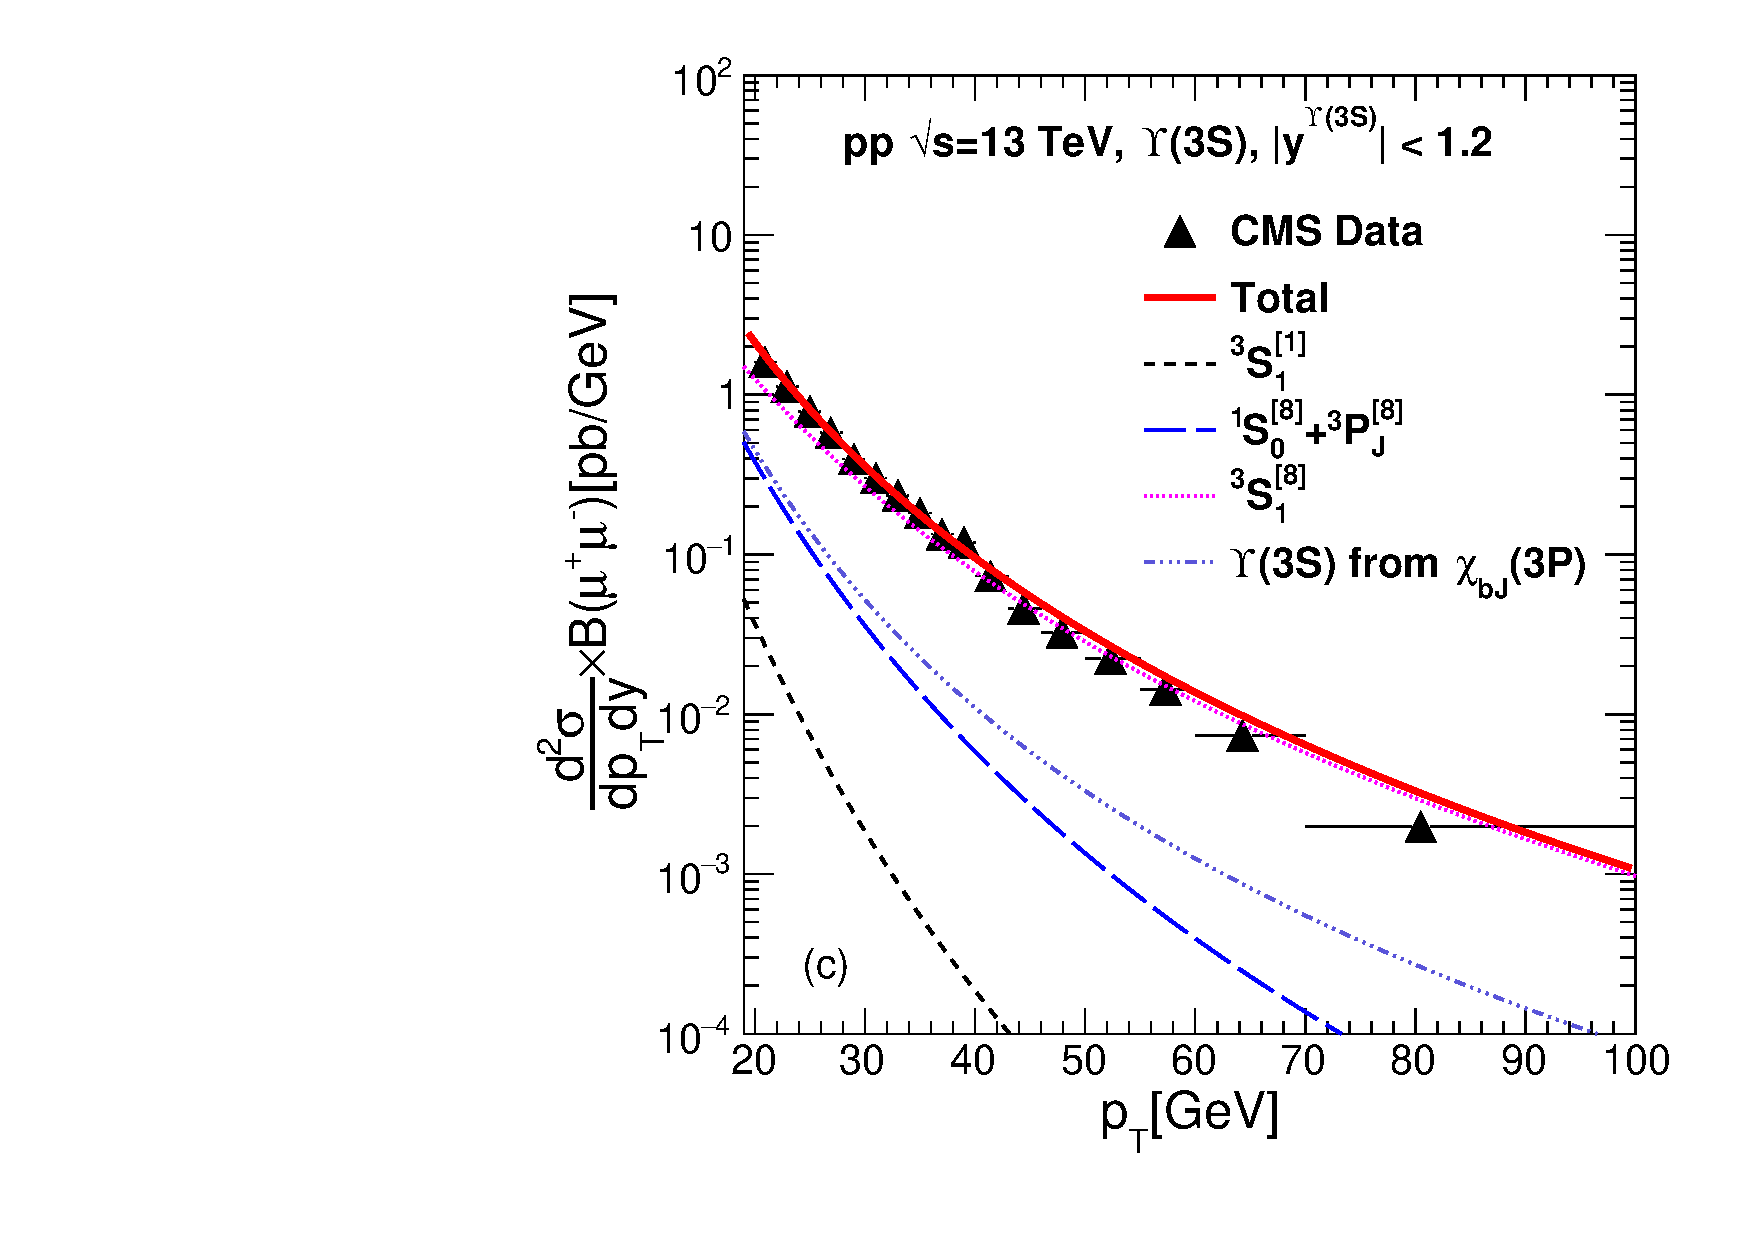
\includegraphics[width=0.49\textwidth]{Figures/NRQCD_Beauty/Fig3c_Y3S_CMS_13TeV_Rap12.pdf}
%  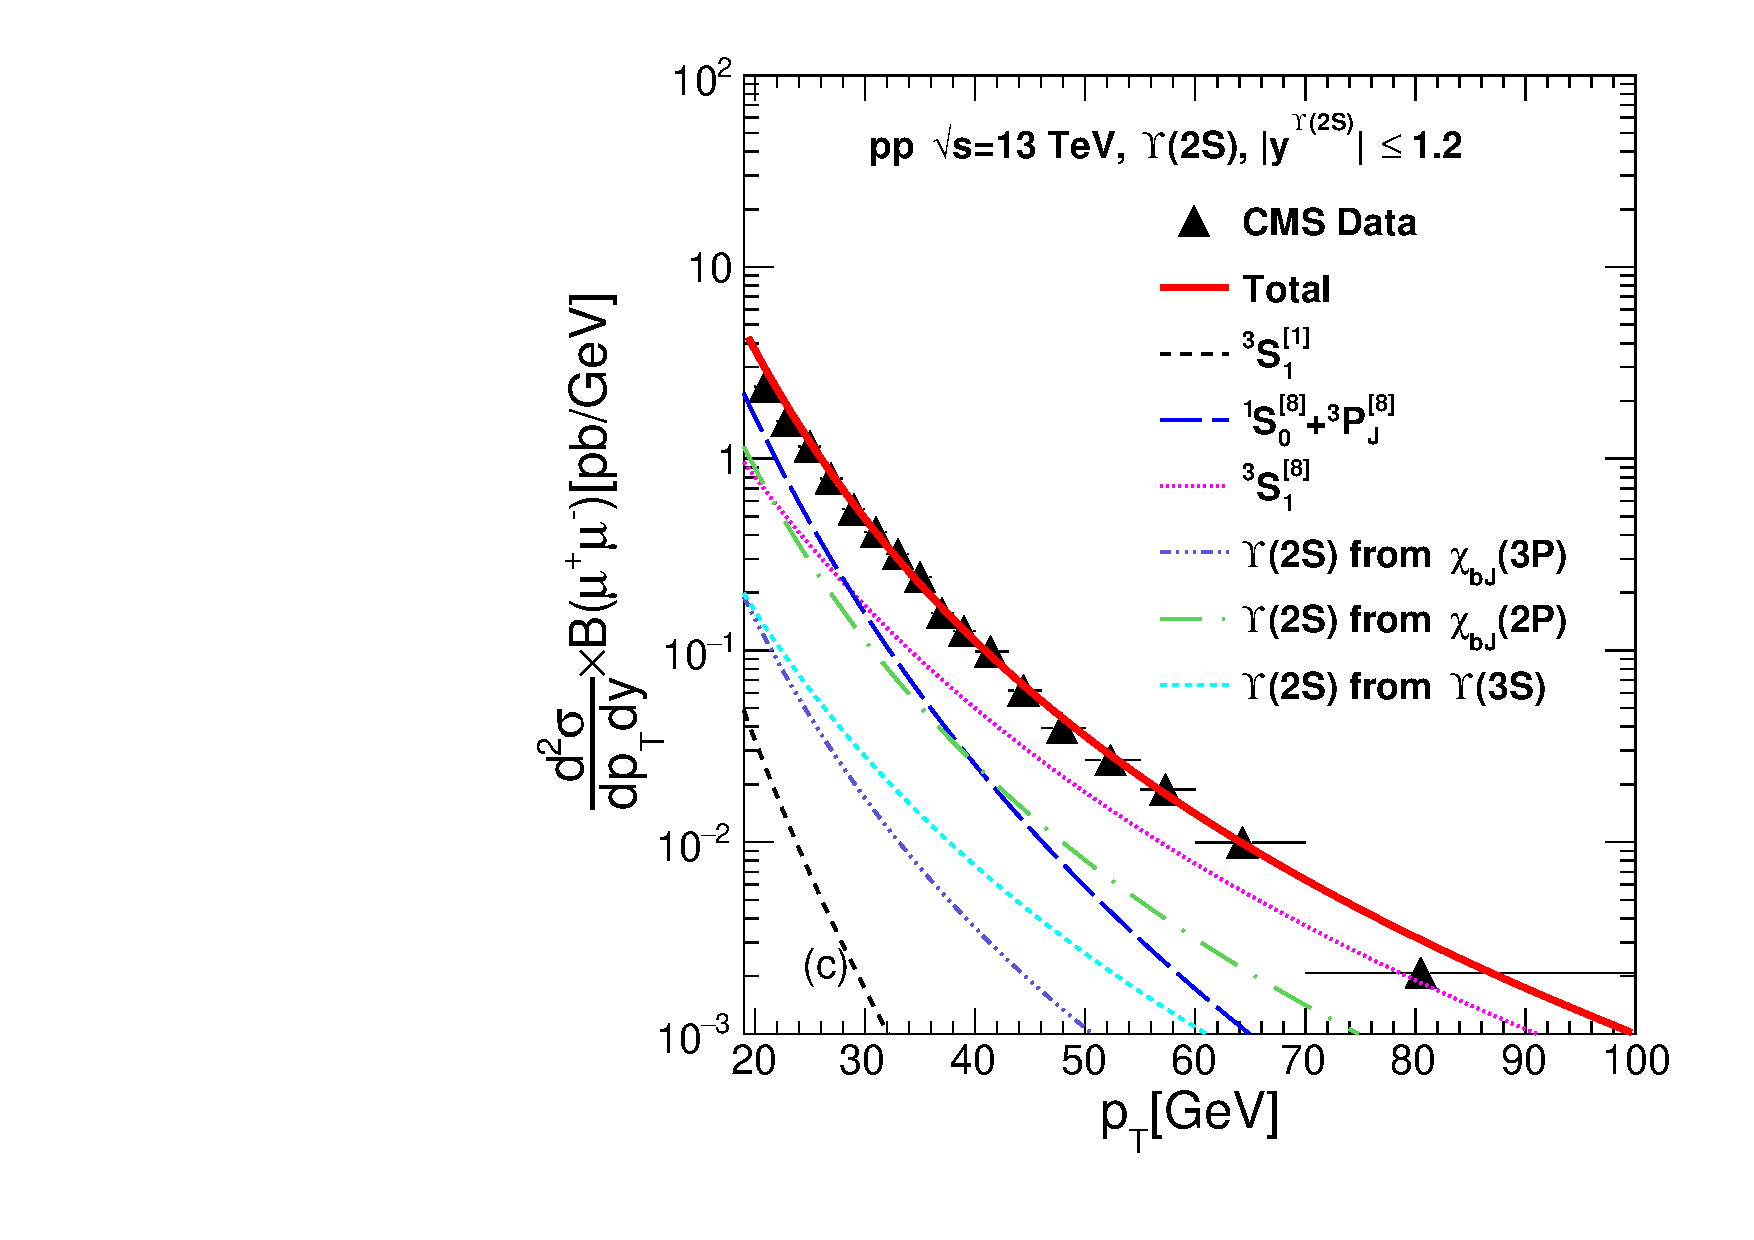
\includegraphics[width=0.49\textwidth]{Figures/NRQCD_Beauty/Fig6c_CMS_D2NDPtDy_Y2S_13TeV_Y0012_Pt.pdf}
%  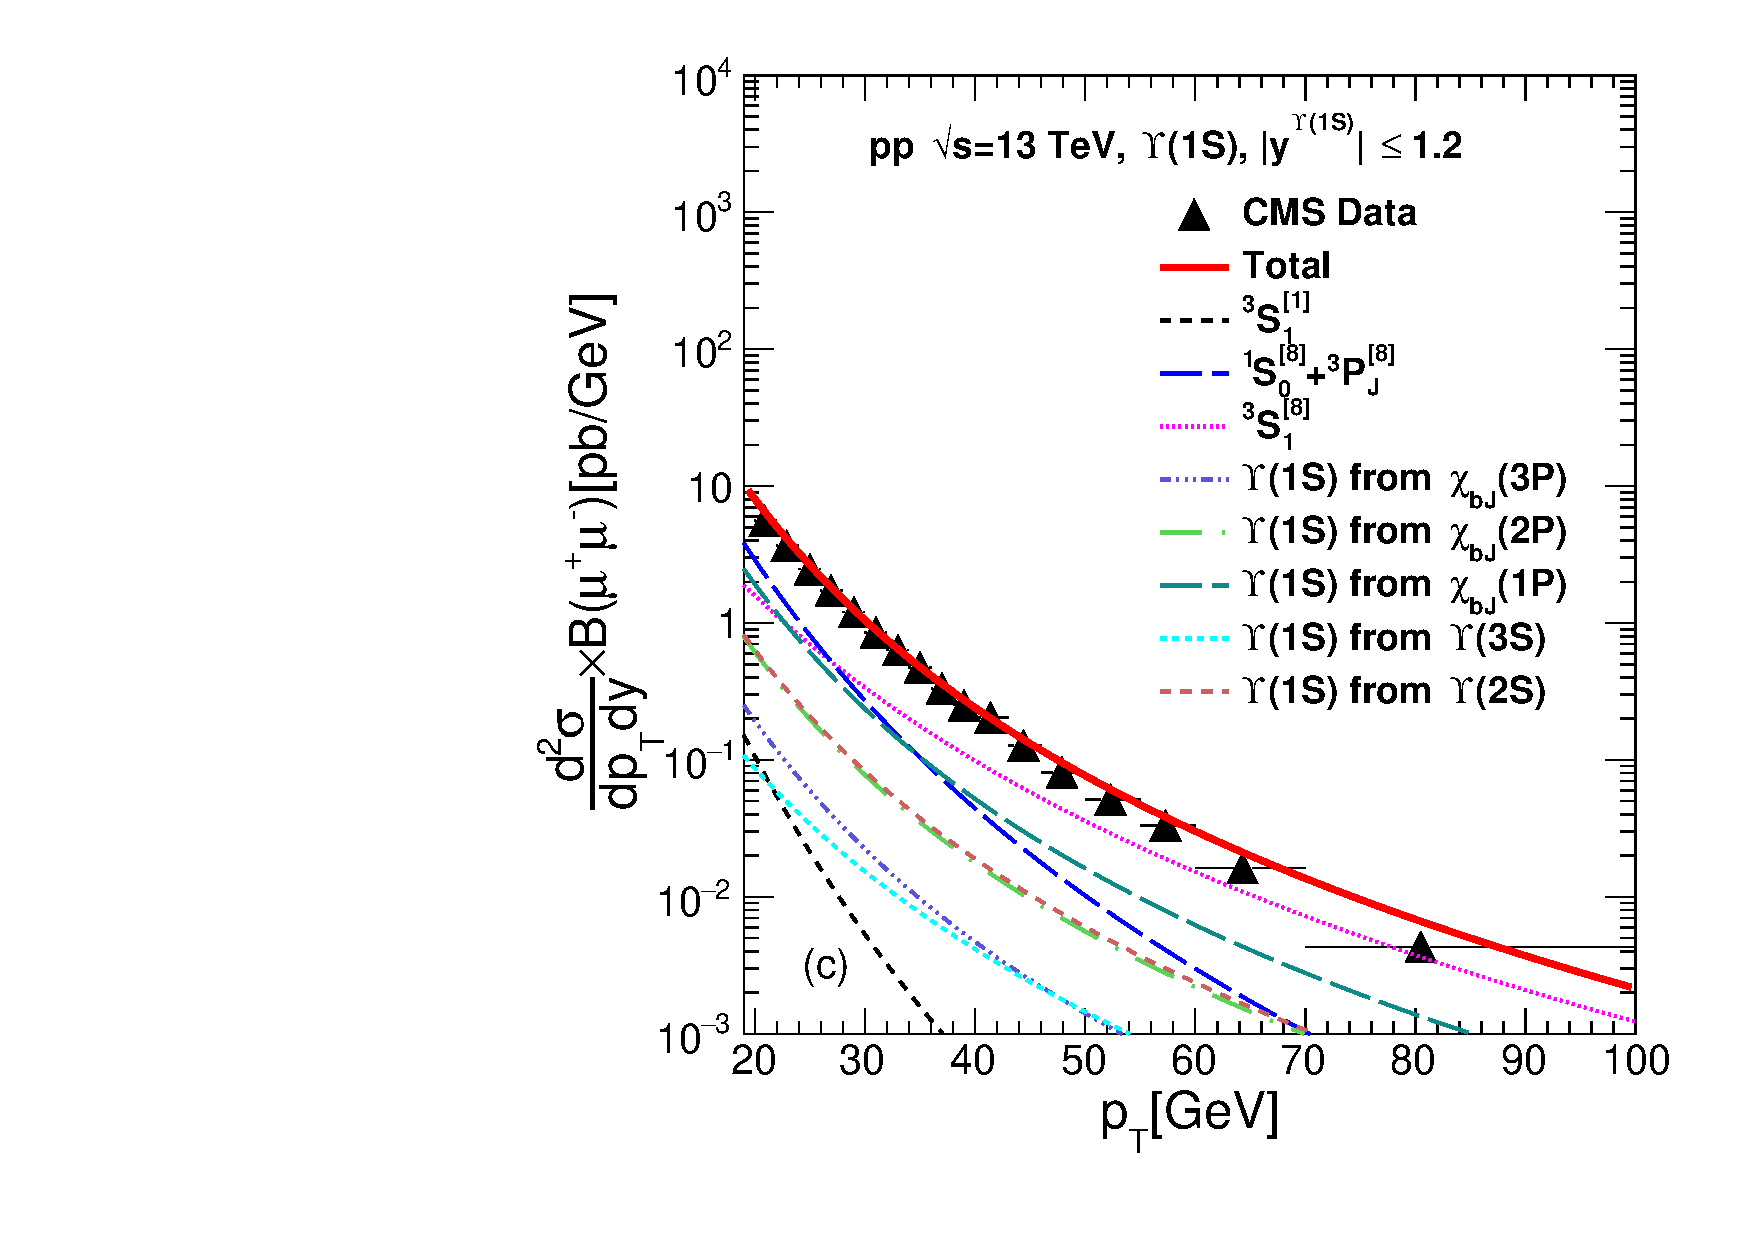
\includegraphics[width=0.49\textwidth]{Figures/NRQCD_Beauty/Fig8c_CMS_D2NDPtDy_Y1S_13TeV_Y0012_Pt.pdf}
%  \caption{\small{The NRQCD calculations of production cross-section of $\Upsilon$(nS) in p+p collisions at 
%      $\sqrt{s}$ = 13 TeV in central rapidities, as a function of transverse momentum compared with the measured data 
%      at CMS~\cite{Sirunyan:2017qdw} experiment.}}
%  %   The LDMEs are obtained by a combined fit of the CMS and ATLAS data.}
%  \label{Fig:SigmaYnSCMS13TeV}
%\end{figure}


%\begin{figure}
%  \centering
%  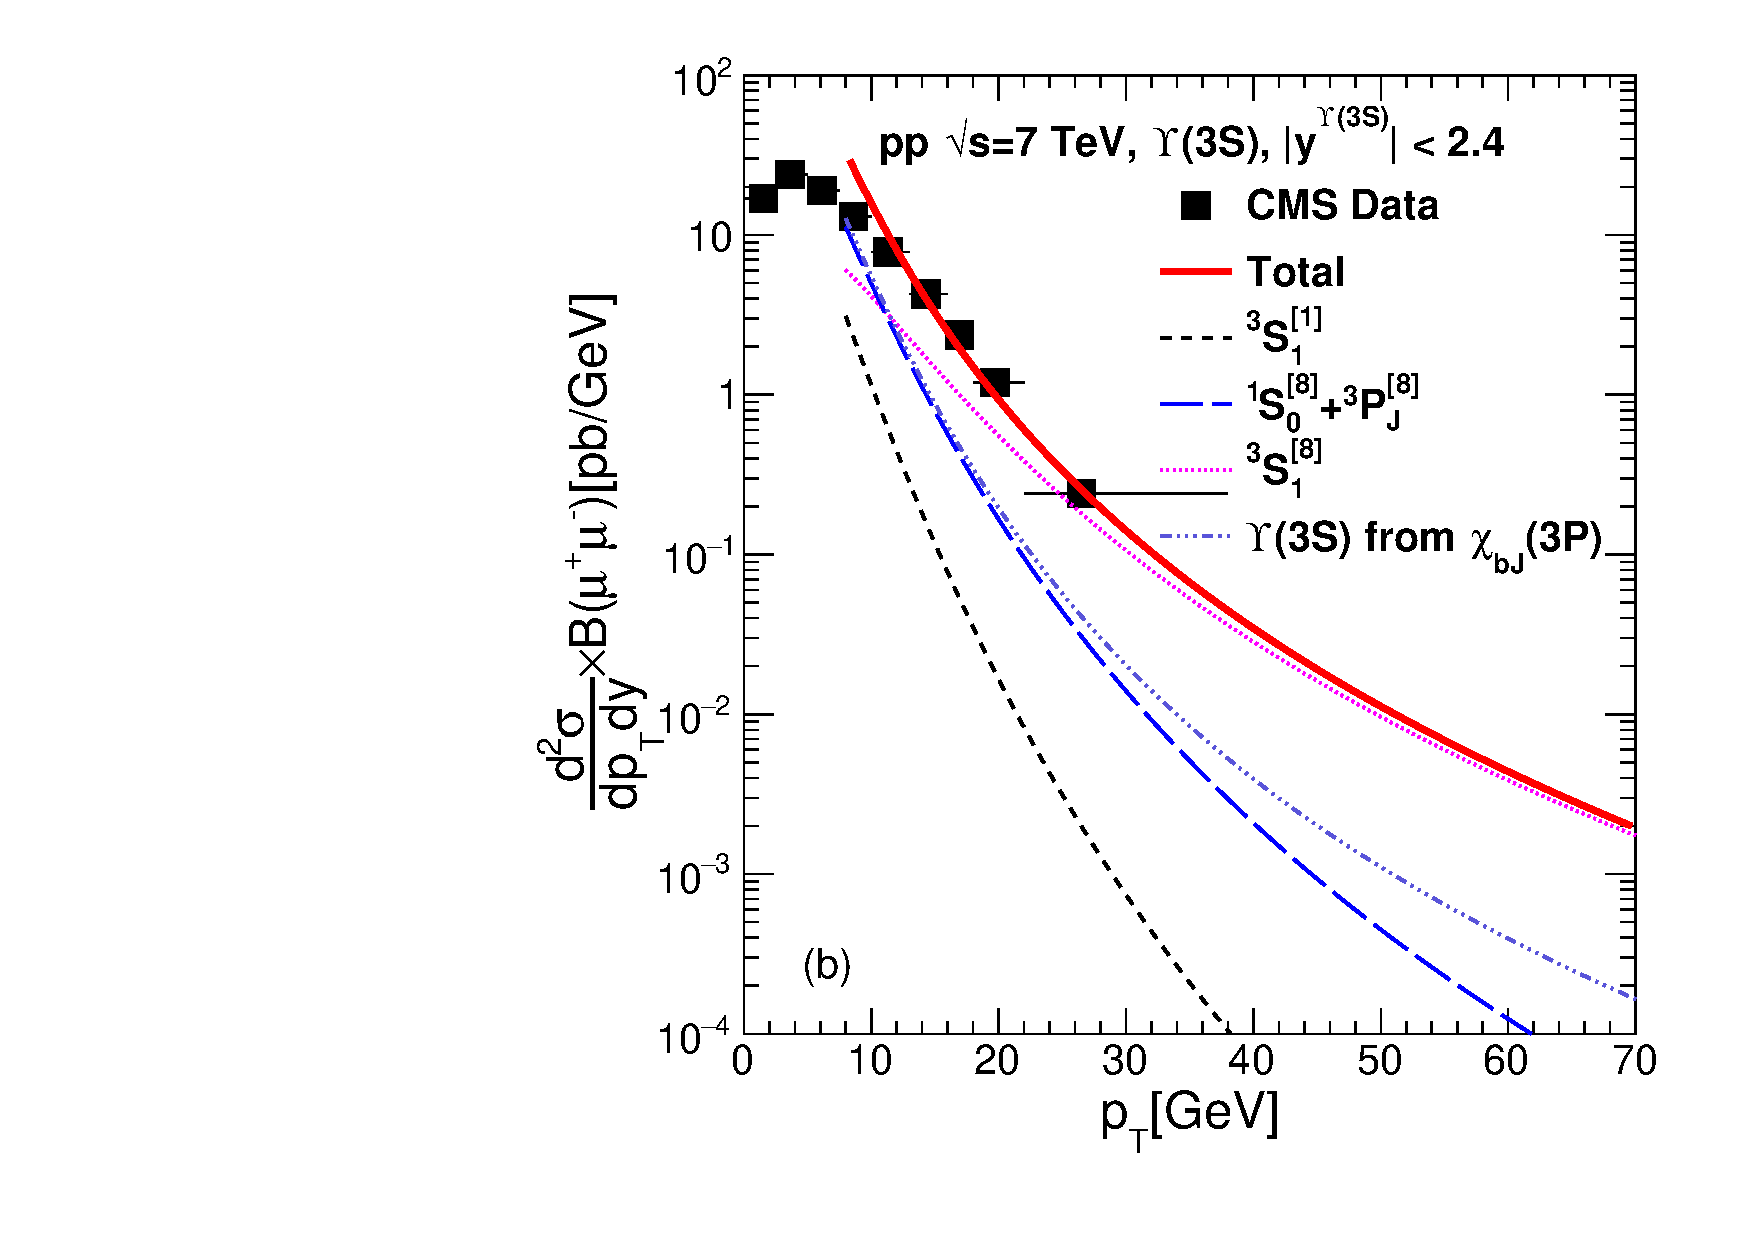
\includegraphics[width=0.49\textwidth]{Figures/NRQCD_Beauty/Fig2b_Y3S_CMS_Rapl24.pdf}
%  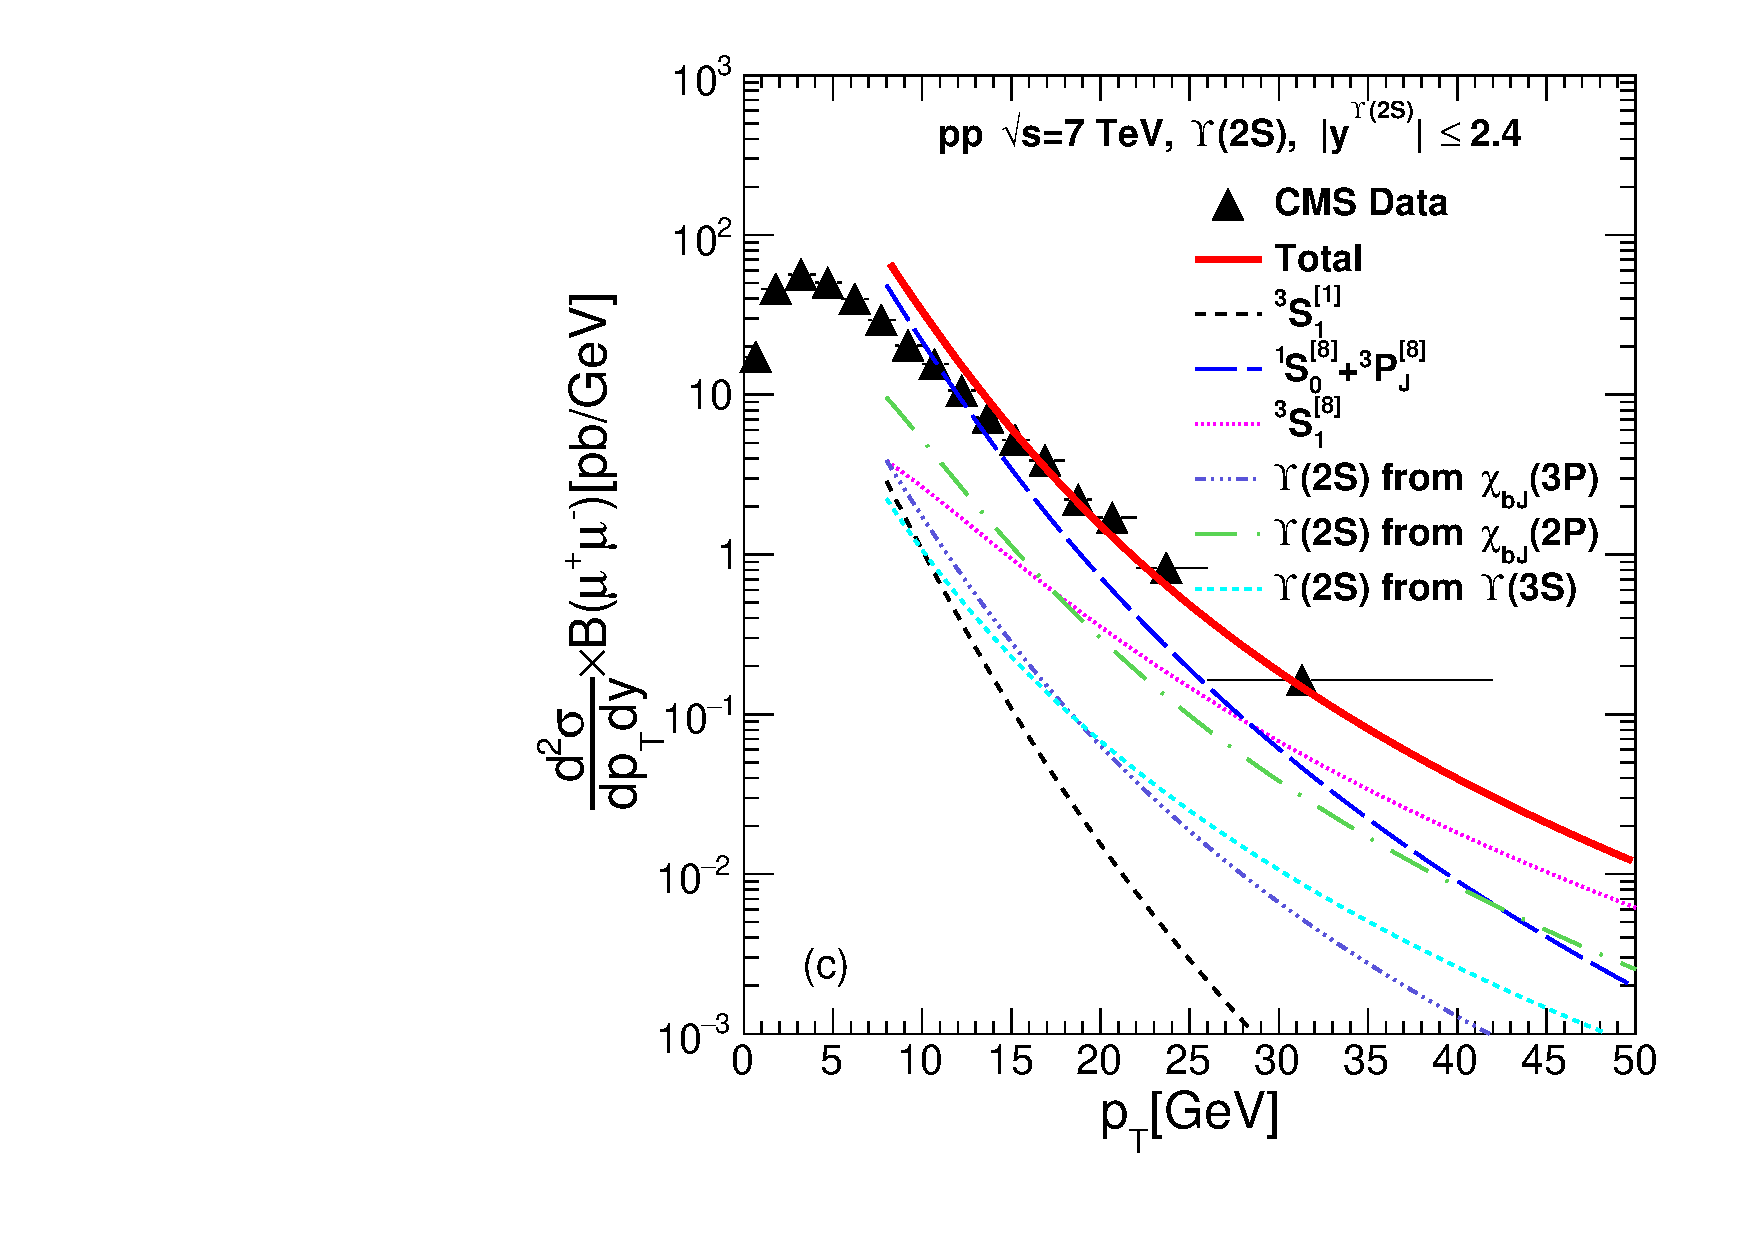
\includegraphics[width=0.49\textwidth]{Figures/NRQCD_Beauty/Fig5c_CMS_D2NDPtDy_Y2S_Y0024_Pt.pdf}
%  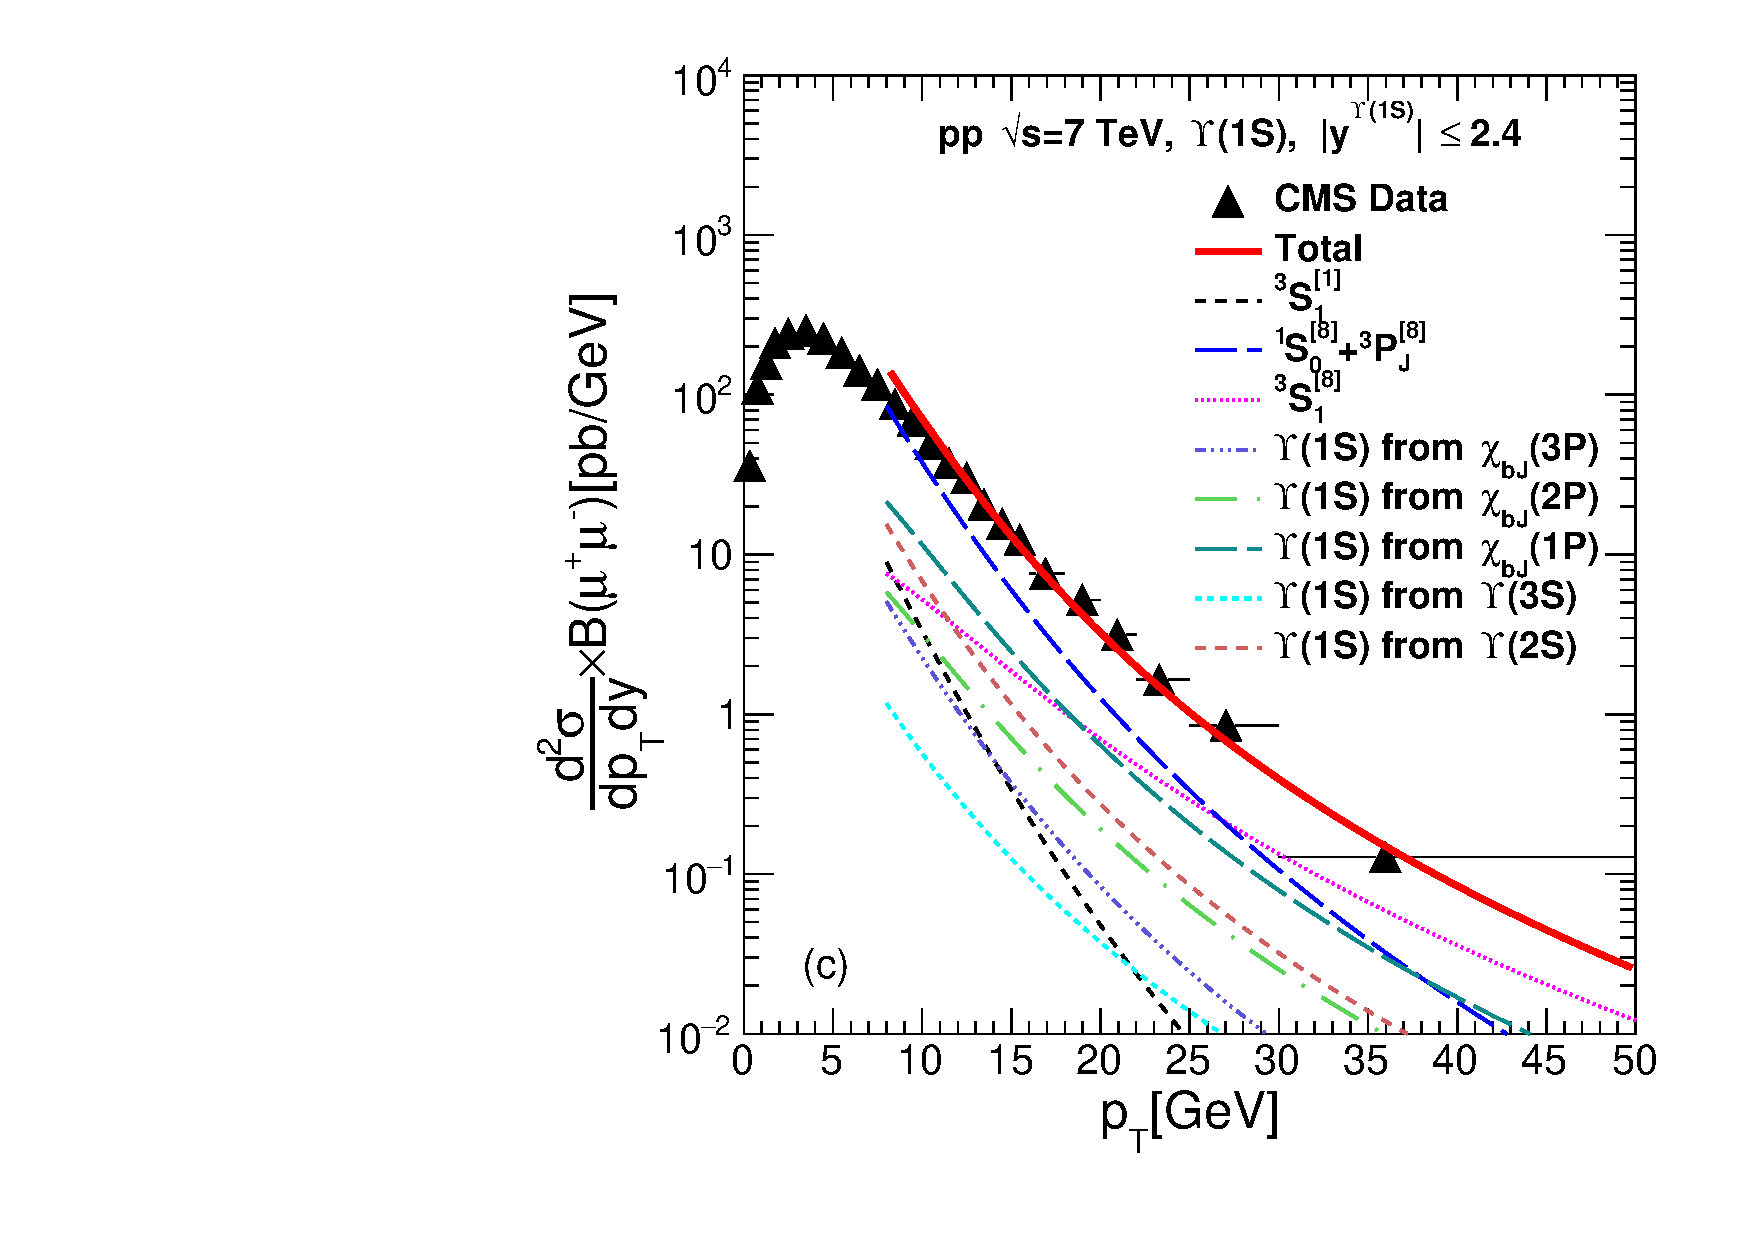
\includegraphics[width=0.49\textwidth]{Figures/NRQCD_Beauty/Fig7c_CMS_D2NDPtDy_Y1S_Y0024_Pt.pdf}
%  \caption{\small{The NRQCD calculations of production cross-section of $\Upsilon$(nS) in p+p collisions at 
%      $\sqrt{s}$ = 7 TeV in central rapidities, as a function of transverse momentum compared with the measured data 
%      at CMS~\cite{Chatrchyan:2013yna} experiment.}}
%  %   The LDMEs are obtained by a combined fit of the CMS and ATLAS data.}
%  \label{Fig:SigmaYnSCMS7TeV}
%\end{figure}

%\begin{figure}
%  \centering
%  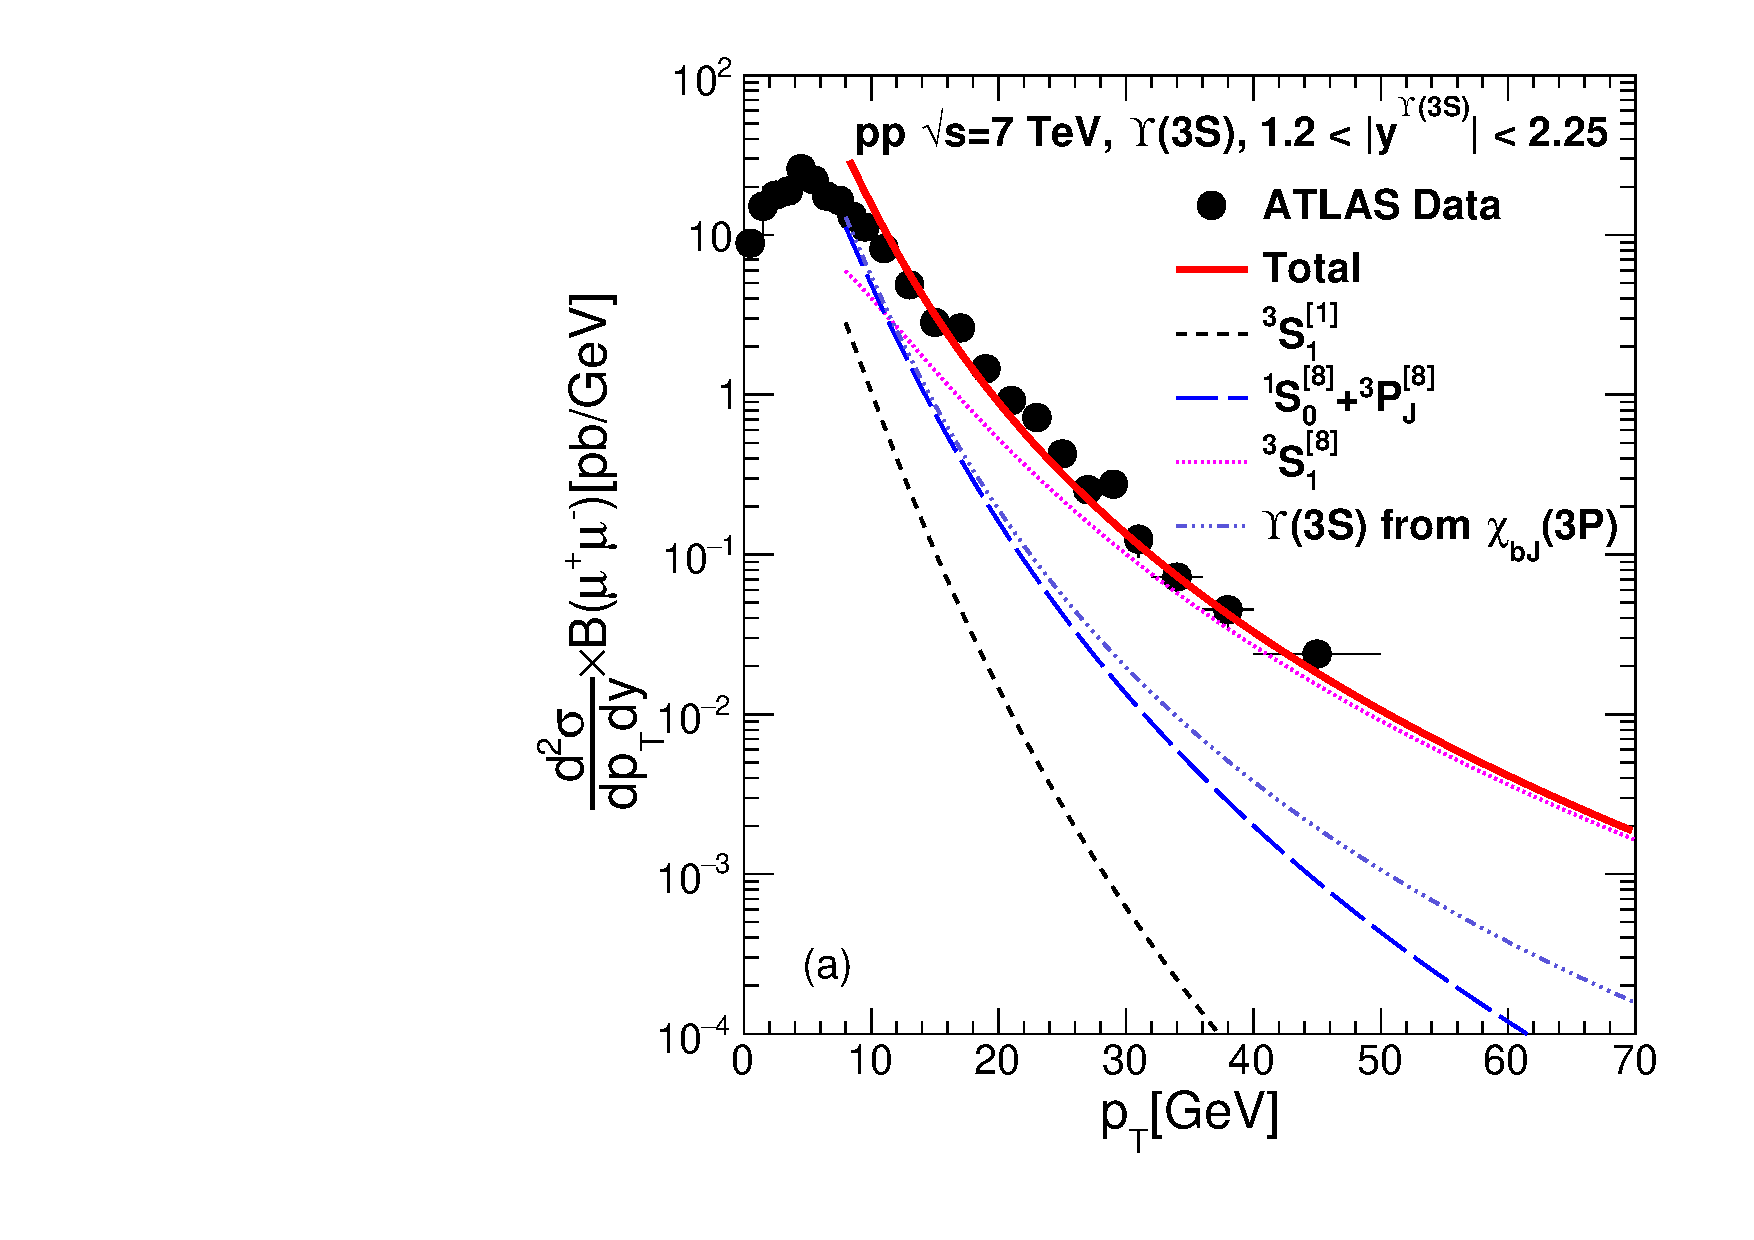
\includegraphics[width=0.49\textwidth]{Figures/NRQCD_Beauty/Fig2a_Y3S_ATLAS_Rap12225.pdf}
%  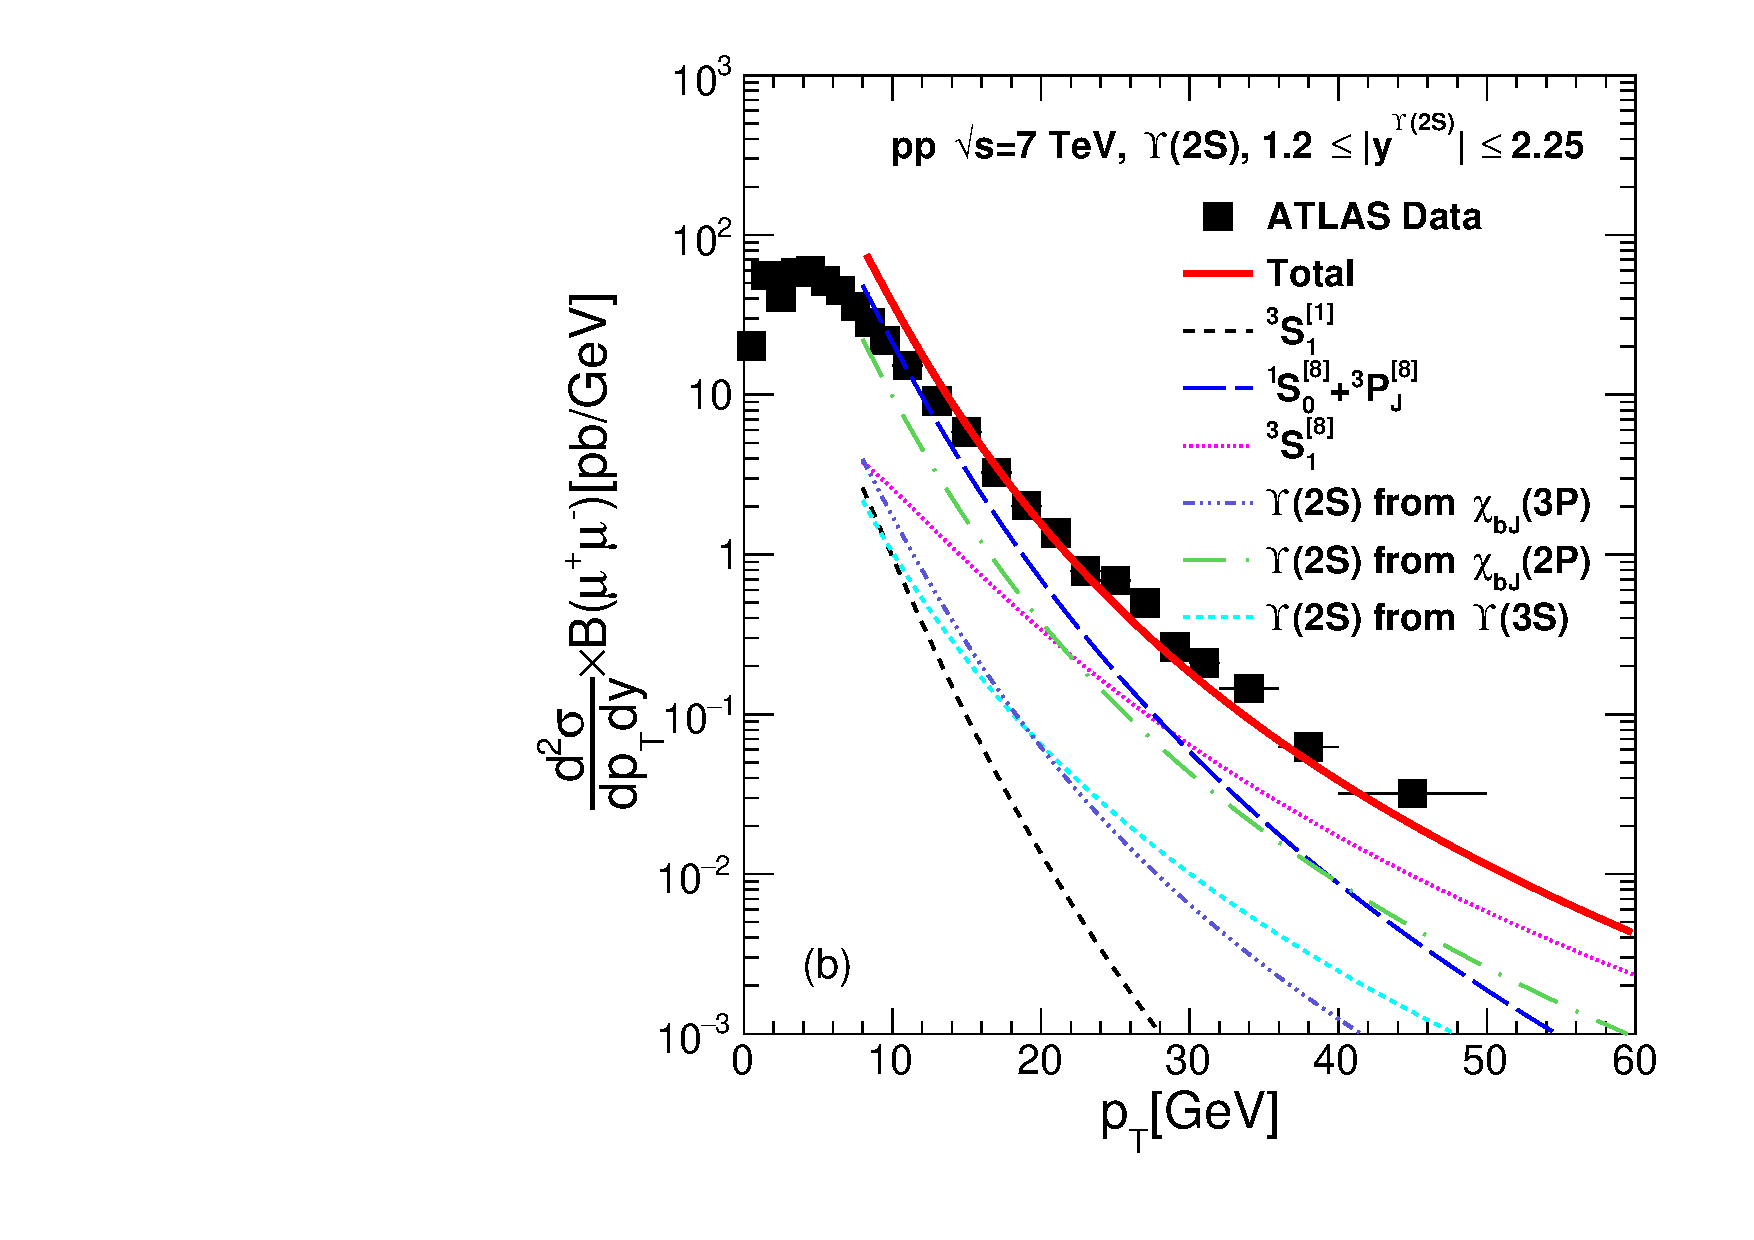
\includegraphics[width=0.49\textwidth]{Figures/NRQCD_Beauty/Fig5b_ATLAS_D2NDPtDy_Y2S_Y12225_Pt.pdf}
%  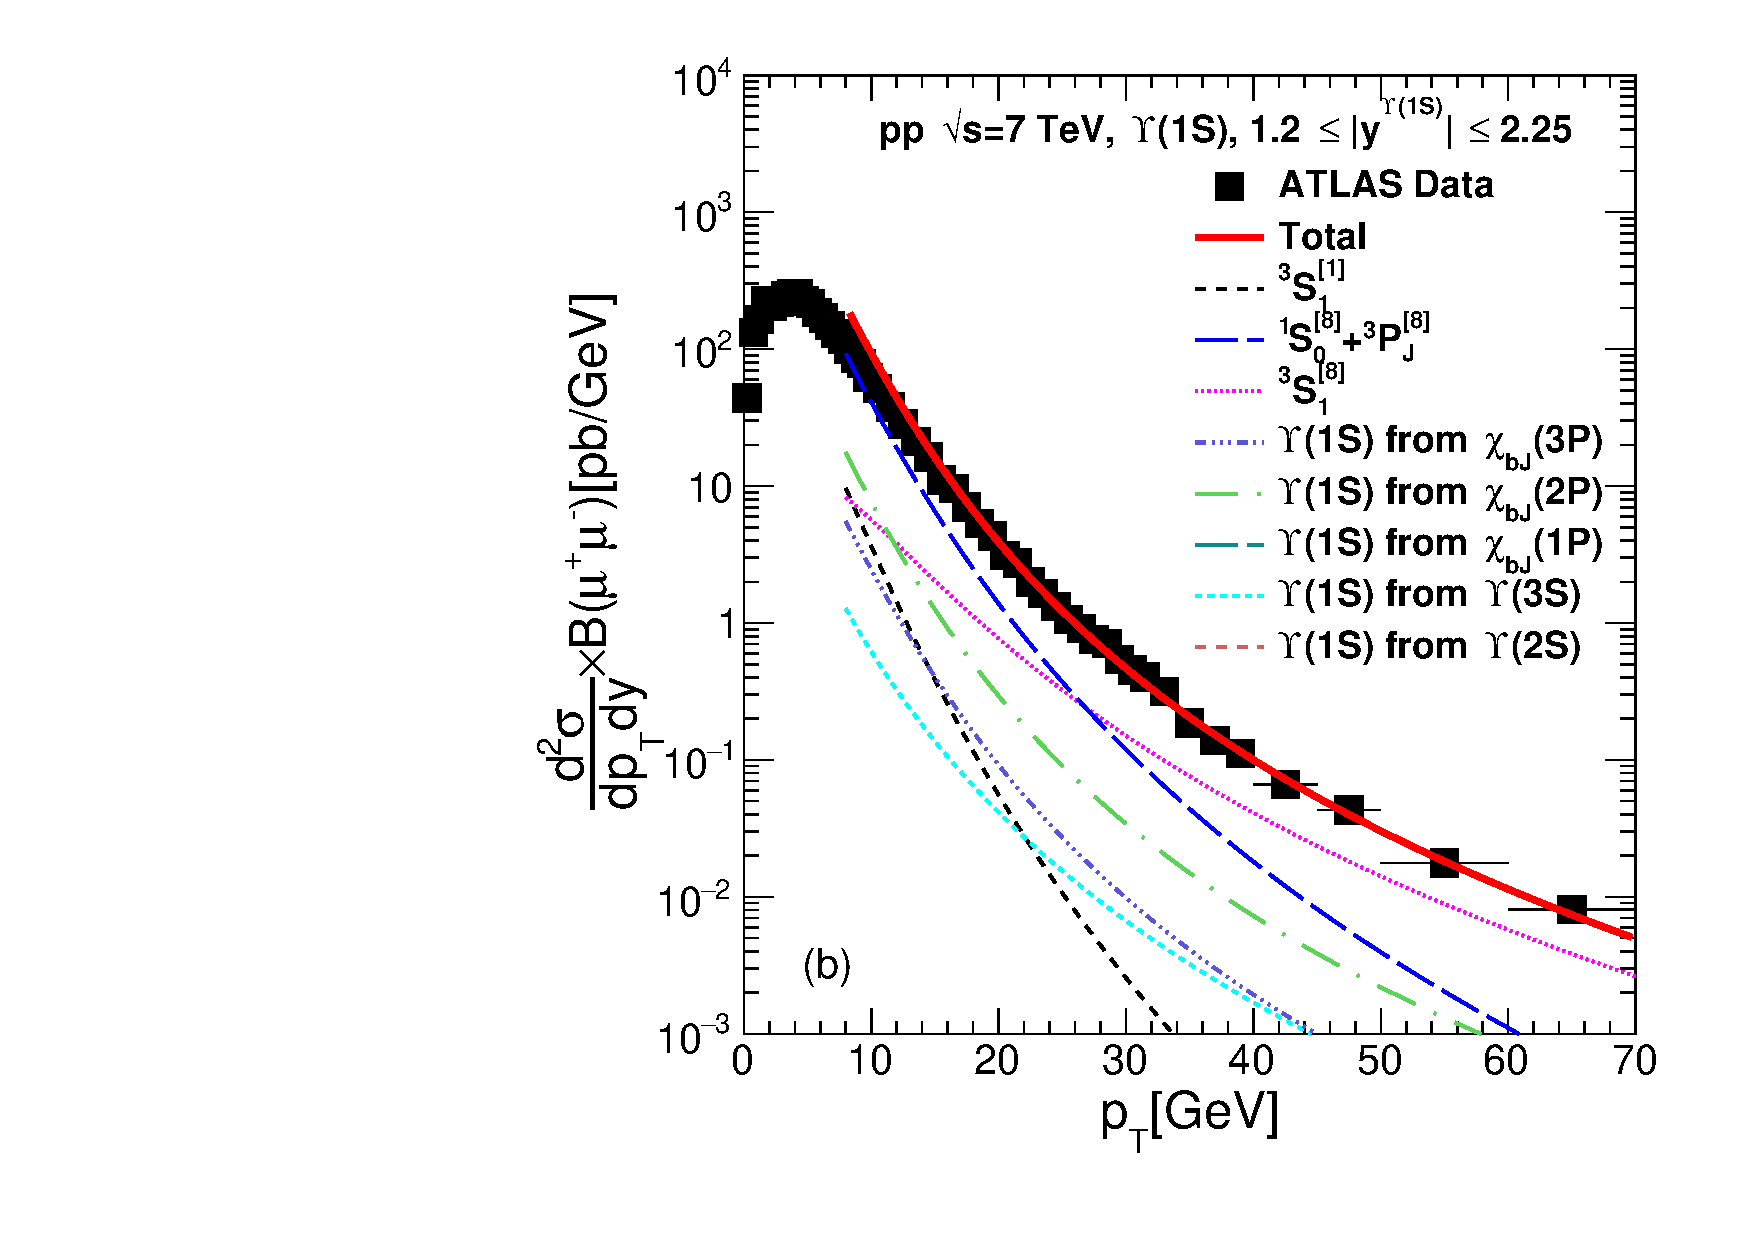
\includegraphics[width=0.49\textwidth]{Figures/NRQCD_Beauty/Fig7b_ATLAS_D2NDPtDy_Y1S_Y12225_Pt.pdf}
%  \caption{\small{The NRQCD calculations of production cross-section of $\Upsilon$(nS) in p+p collisions at 
%      $\sqrt{s}$ = 7 TeV in central rapidities, as a function of transverse momentum compared with the measured data 
%      at ATLAS~\cite{Aad:2012dlq} experiment.}}
%  %   The LDMEs are obtained by a combined fit of the CMS and ATLAS data.}
%  \label{Fig:SigmaYnSATLAS7TeV}
%\end{figure}


\begin{figure}
  \centering
  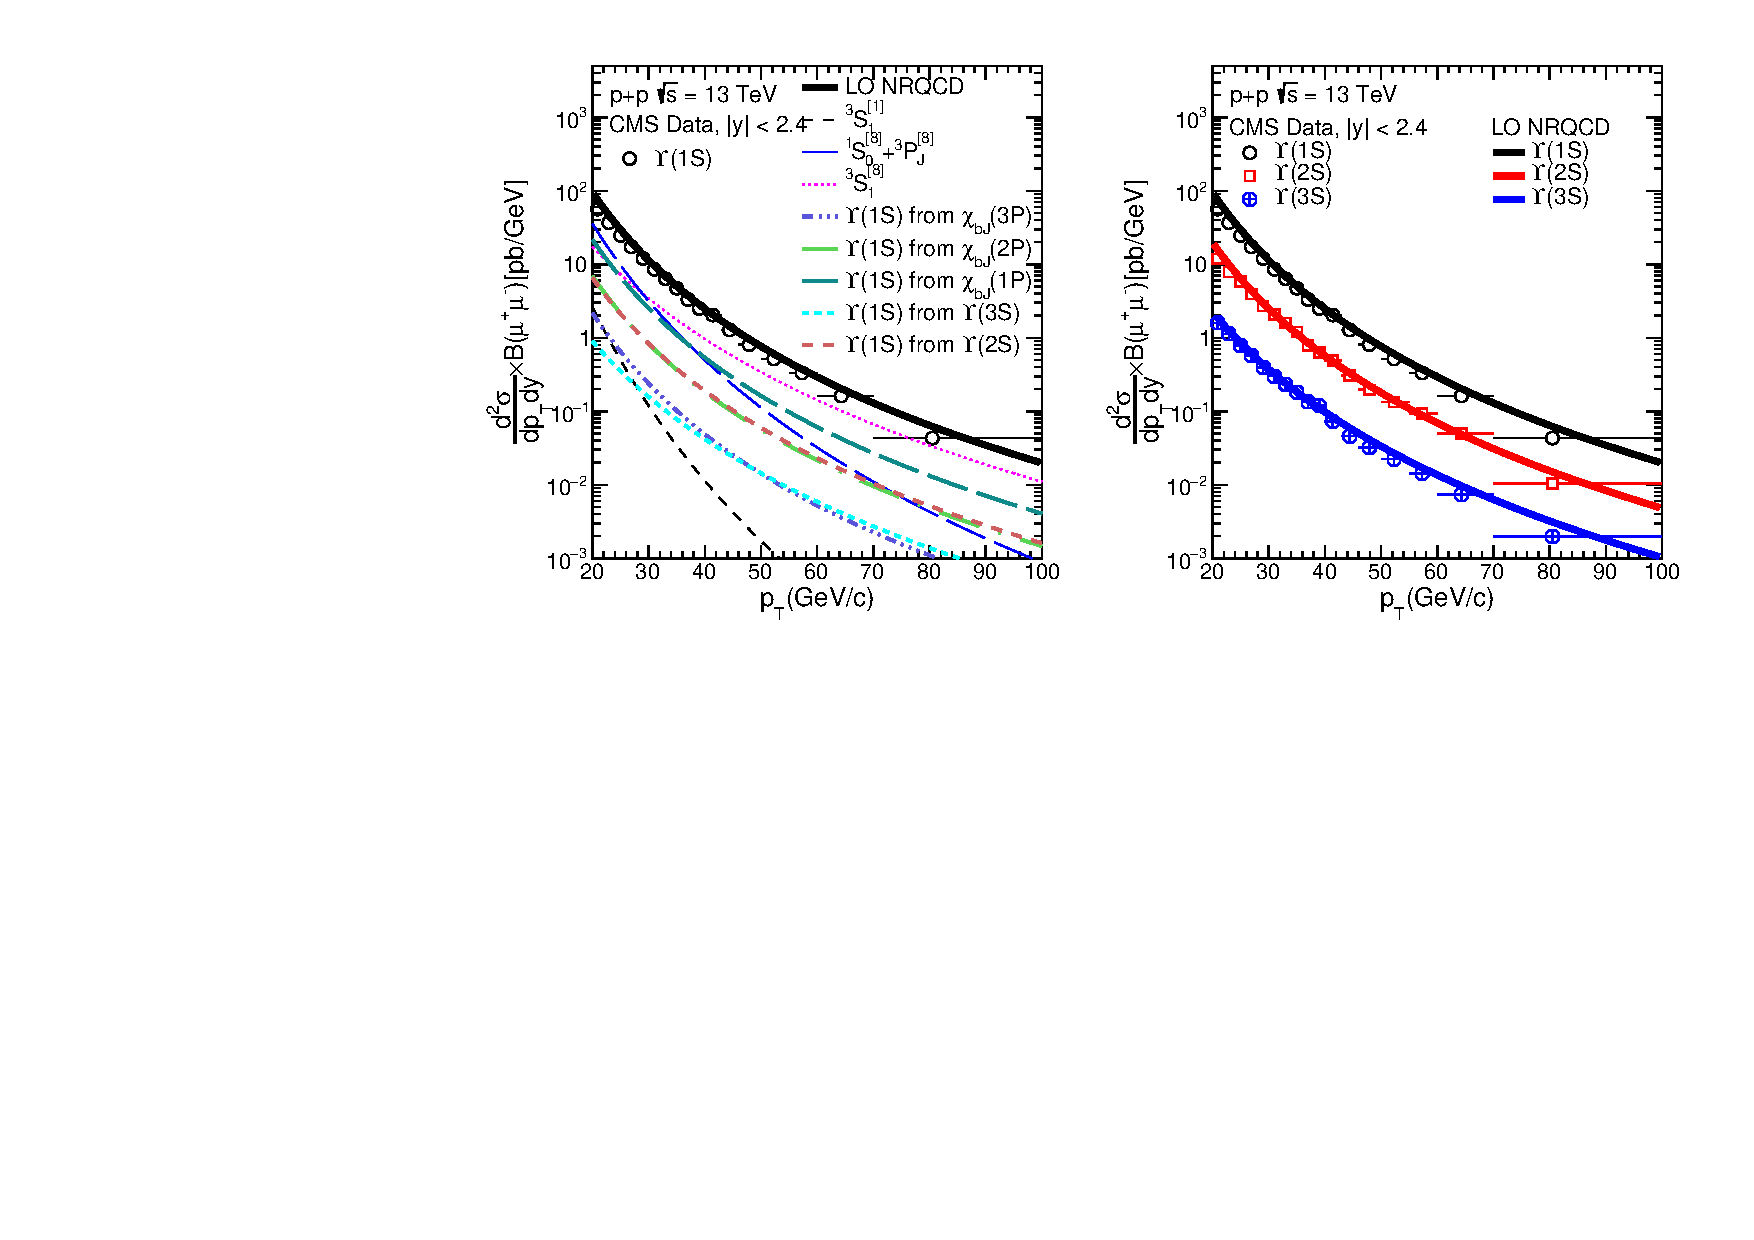
\includegraphics[width=0.99\textwidth]{Figures/NRQCD_Beauty/Fig_CMS_YnS_Rap12_13TeV_Pt.pdf}
  \caption{\small{The NRQCD calculations of production cross-section of $\Upsilon$(nS)
      in p+p collisions at $\sqrt{s}$ = 13 TeV in central rapidities, as a function of
      transverse momentum compared with the measured data at CMS~\cite{Sirunyan:2017qdw}
      experiment. The left figure shows relative contributions in $\Upsilon$(1S) from
      singlet and octet states as well as from feeddown. The right figure shows the sum
      of all contributions for all the 3 states where the results for $\Upsilon$(1S) and
      $\Upsilon$(2S) are shifted vertically by a constant factor for better visibility. } }
  %   The LDMEs are obtained by a combined fit of the CMS and ATLAS data.}
  \label{Fig:SigmaYnSCMS13TeV}
\end{figure}



\begin{figure}
  \centering
  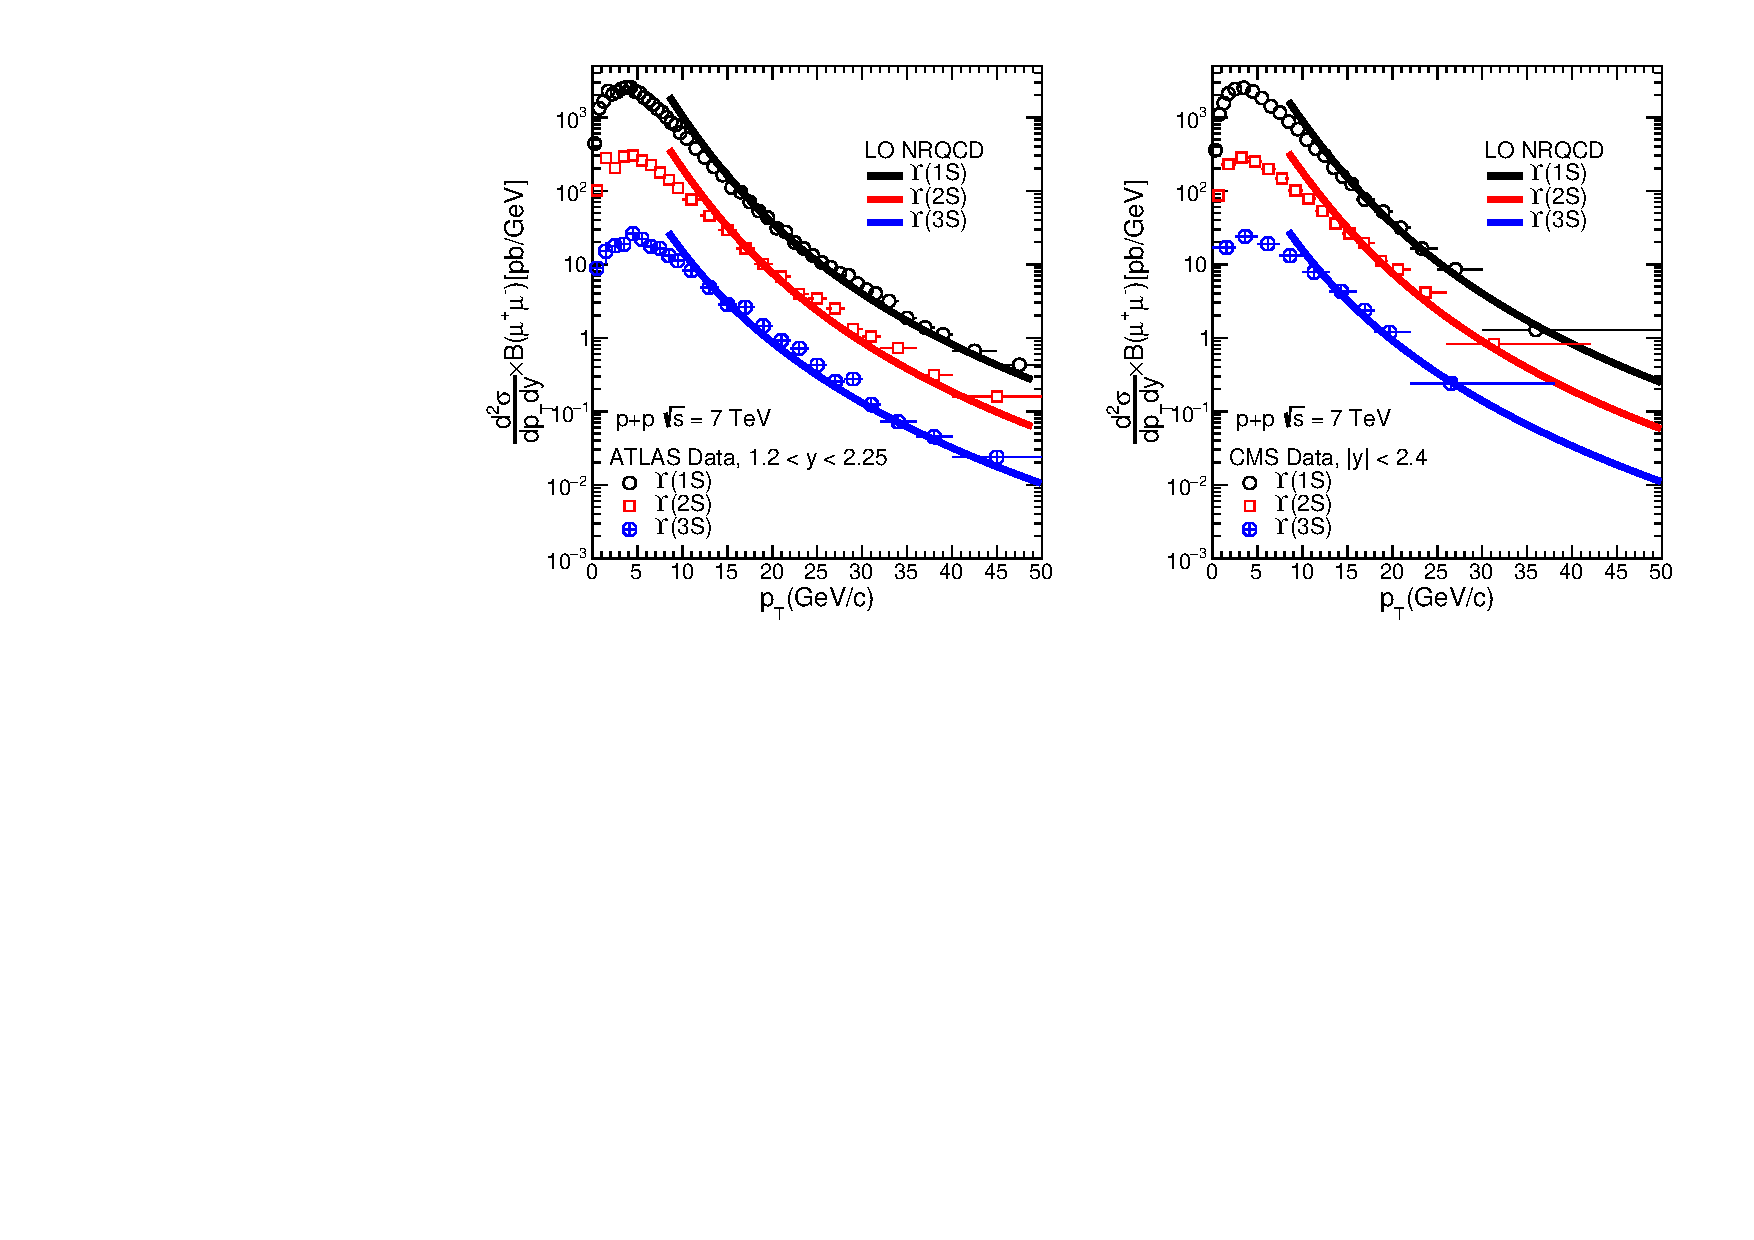
\includegraphics[width=0.99\textwidth]{Figures/NRQCD_Beauty/Fig_CMS_ATLAS_YnS_7TeV_Pt.pdf}
  \caption{\small{The NRQCD calculations of production cross-section of $\Upsilon$(nS) in
      p+p collisions at $\sqrt{s}$ = 7 TeV, as a function of transverse momentum compared with
      the measured data by ATLAS~\cite{Aad:2012dlq} in left figure and CMS~\cite{Chatrchyan:2013yna}
      in right figure. The cross-section of $\Upsilon$(1S) and $\Upsilon$(2S) as well as
      calculations are shifted vertically by a constant factor for better visibility.}}
  %   The LDMEs are obtained by a combined fit of the CMS and ATLAS data.}
  \label{Fig:SigmaYnSCMS7TeV}
\end{figure}



The NRQCD formalism provides an adequate procedure to estimate a quantity as an expansion in 
heavy quark relative velocity, $v$ inside $Q\bar{Q}$ bound state. The LDME in Eq.(\ref{eq6})
do scale with definitive power in $v$. The quarkonium yield depends on the $^3S_1^{[1]}$ 
and $^3P_J^{[1]}$(J=0,1,2) CS states and $^1S_0^{[8]}$, $^3S_1^{[8]}$ and $^3P_J^{[8]}$
CO states in the limit $v\ll 1$.
%The quantity in the $[]$ stands for angular momentum
%quantum numbers of the meson in Fock expansion, whereas
The superscripts in square brackets represent the colour structure of the bound state,
1 for the CS and 8 for the CO.


%It is assumed that there is no significant feed down effect in $\Upsilon$(3S) from
%higher mass states like $\chi_{bJ}$(3P).

%\begin{figure}[!h]
%  \centering
%  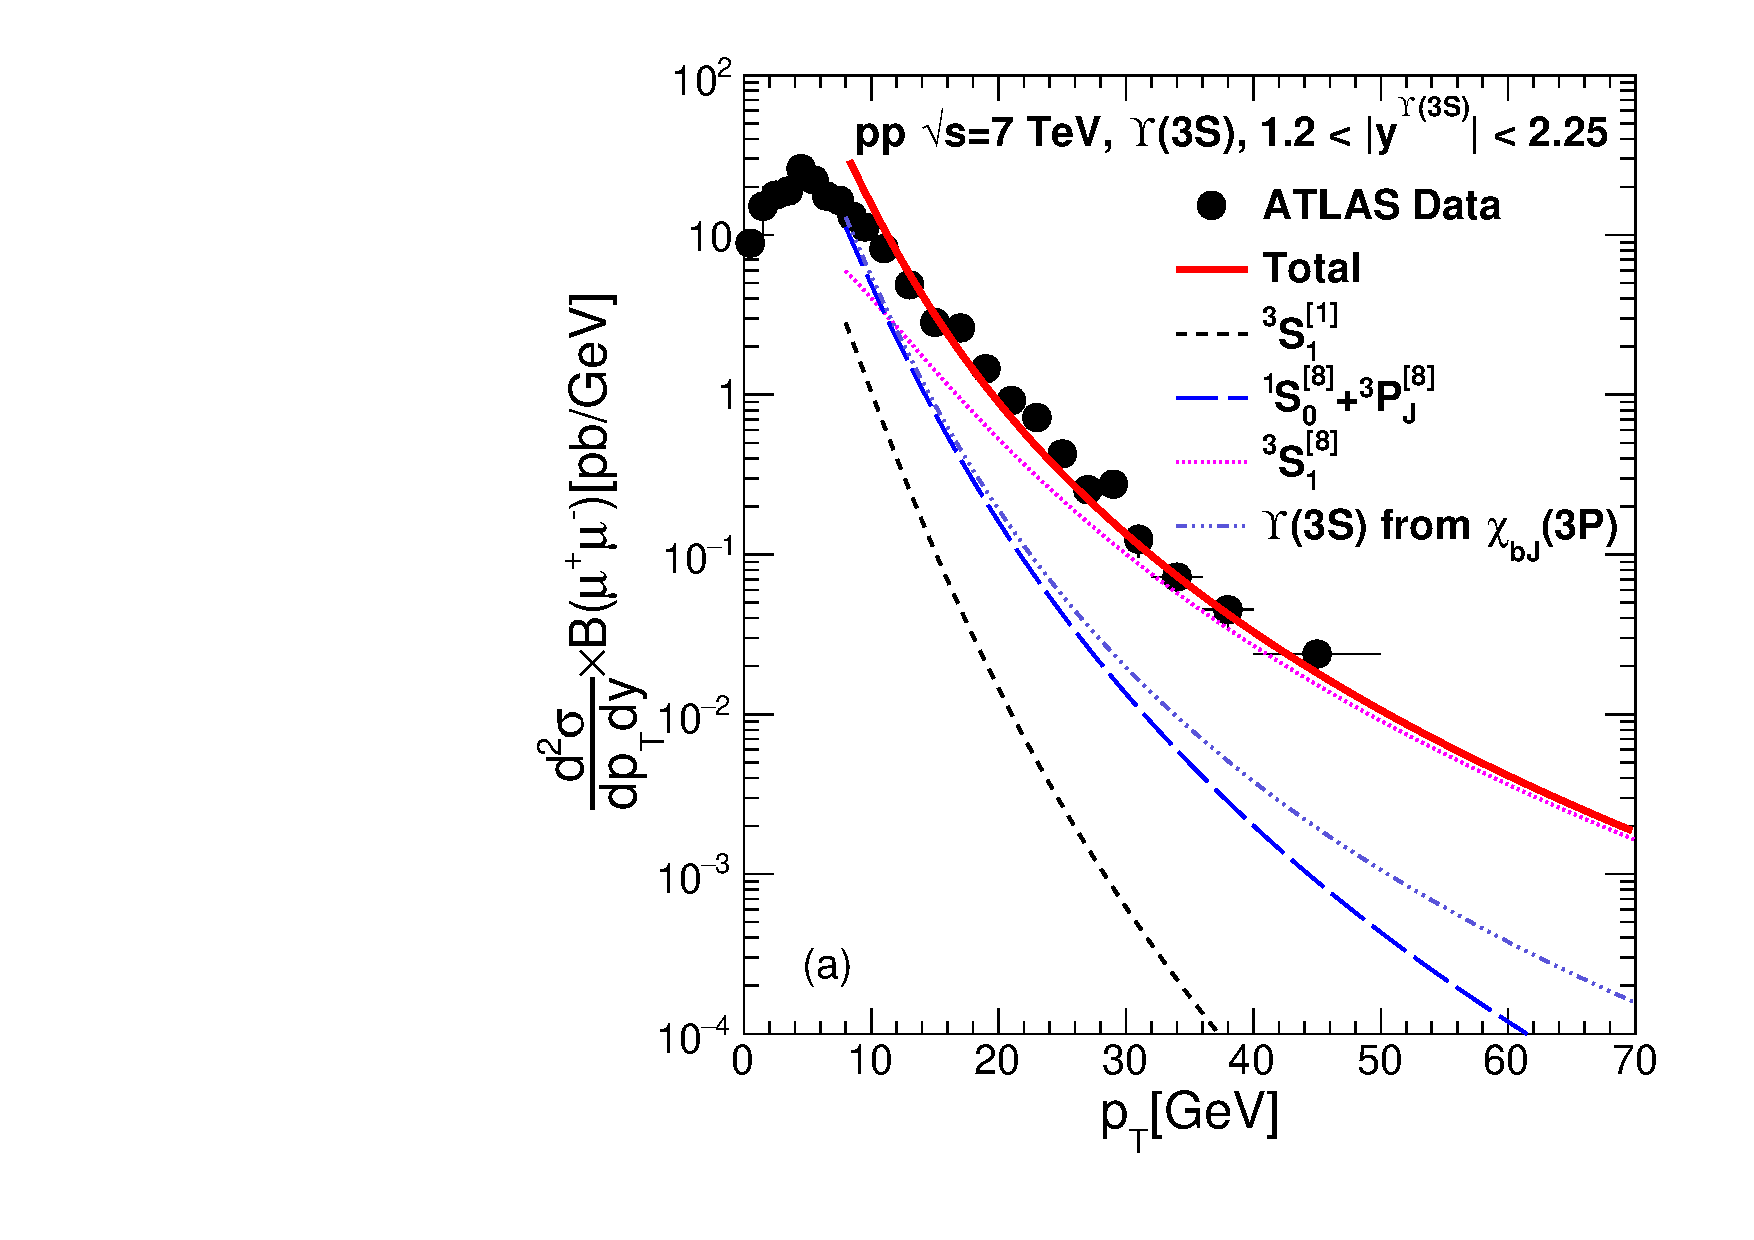
\includegraphics[width=0.49\textwidth]{Figures/NRQCD_Beauty/Fig2a_Y3S_ATLAS_Rap12225.pdf}
%  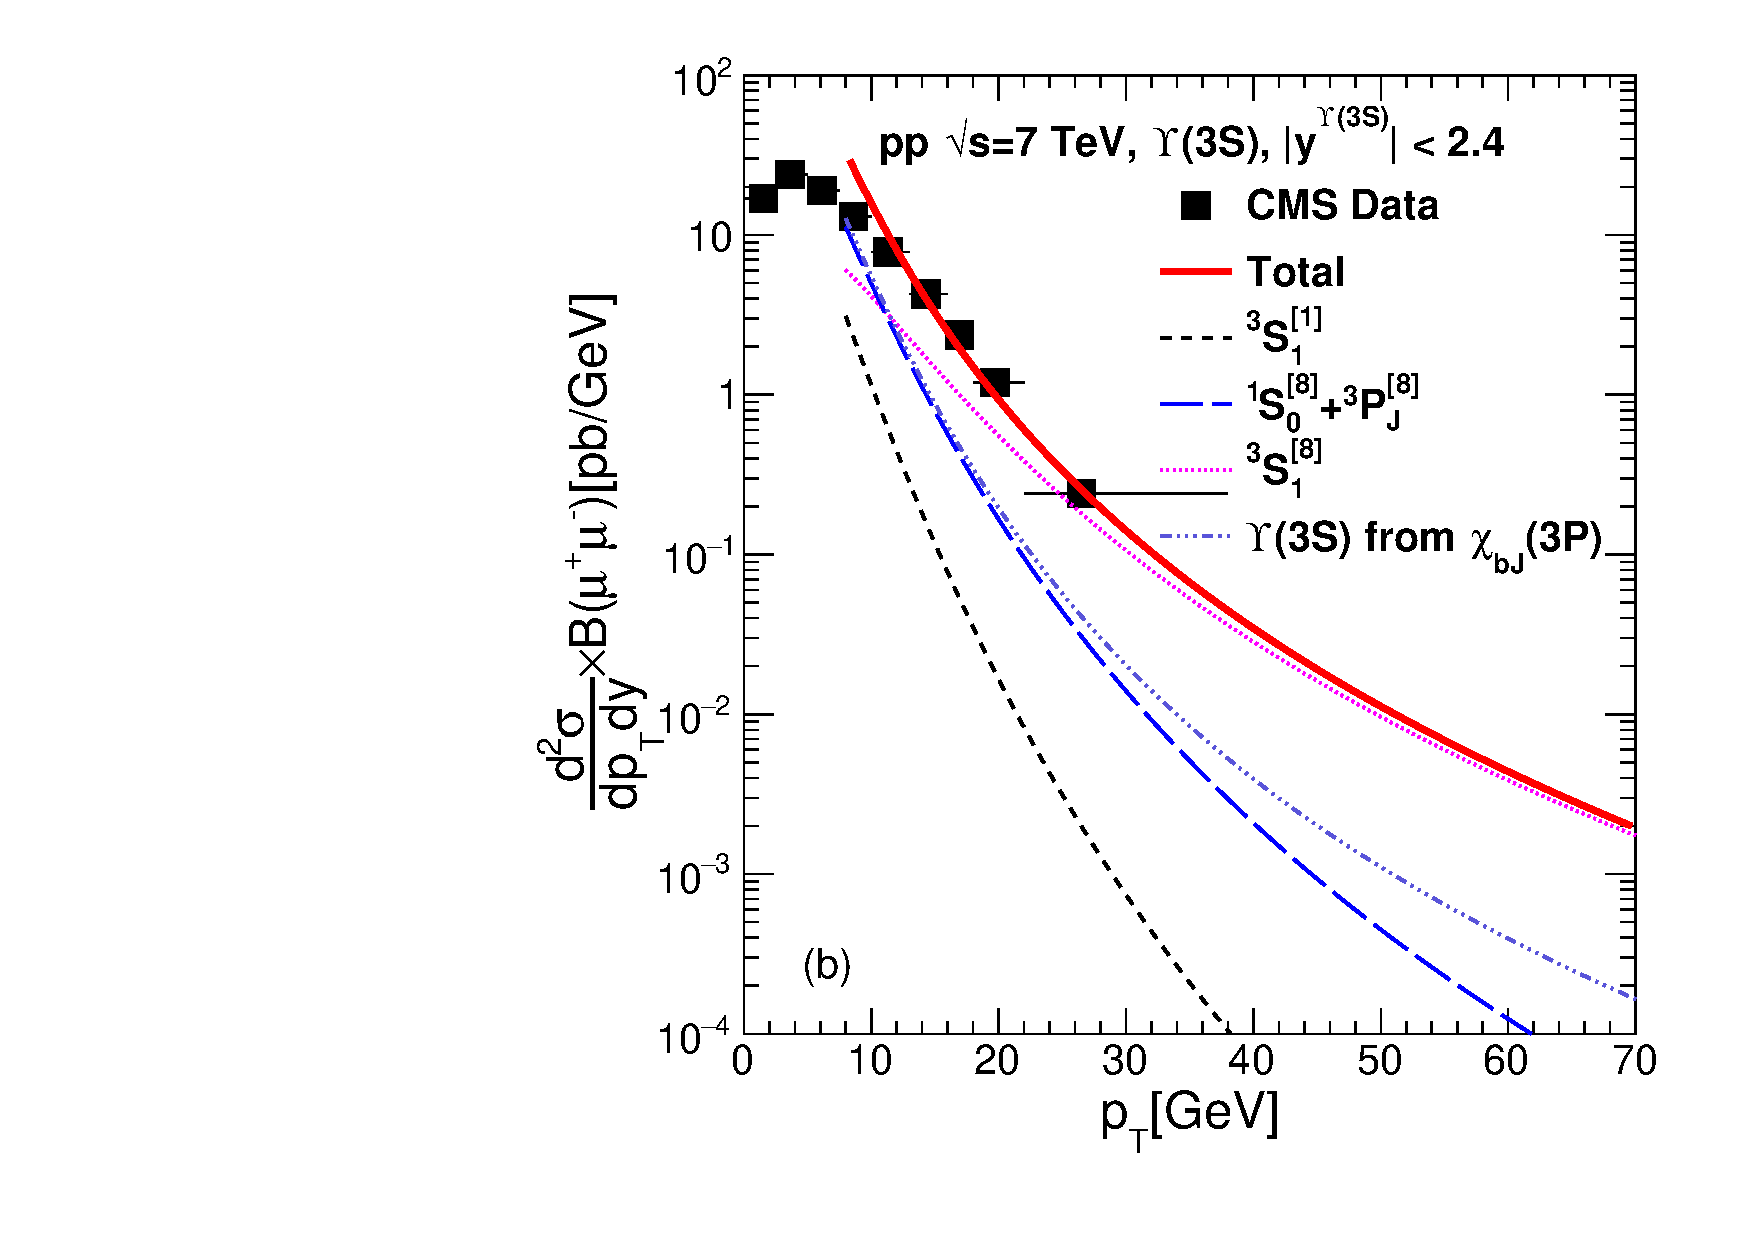
\includegraphics[width=0.49\textwidth]{Figures/NRQCD_Beauty/Fig2b_Y3S_CMS_Rapl24.pdf} 
%  \caption{\small{The NRQCD calculations of production cross-section of $\Upsilon$(3S) in p+p collisions at 
%      $\sqrt{s}$ = 7 TeV in forward rapidities, as a function of transverse momentum compared with the measured data 
%      at ATLAS~\cite{Aad:2012dlq} and CMS~\cite{Chatrchyan:2013yna} experiments. }}
%  %   The LDMEs are obtained by a combined fit of the CMS and ATLAS data.}
%  \label{Fig:SigmaY3SCMS_forwardRap}
%\end{figure}


We require both CS and CO matrix elements in order to get theoretical
predictions for the production of bottomonia at the Tevatron and LHC energies.
The corresponding expressions and
numerical values for CS states are obtained from Ref.~\cite{Braaten:2000cm}.
The CO states, on the other hand, cannot be directly connected to the non-relativistic
wavefunctions of heavy mesons,
as these are associated with a higher Fock state. Experimentally measured data sets are 
therefore employed to obtain them as in Refs.~\cite{Braaten:2000cm,Cho:1995vh,Cho:1995ce}. 
%The CS operators along with their theoretical values
%and the CO operators to be fitted are listed in Table~\ref{CSCO},
%where, $n$=1,2,3.
For the CO elements related to p-wave states, needed as the 
feed down contributions, we have used values obtained by Ref.~\cite{Sharma:2012dy,Feng:2015wka} for the 
present purpose. In our calculations, we have used
%CTEQ6L parametrisation \cite{Lai:2010vv} for parton distribution functions and
CT18NLO parametrisation~\cite{Hou:2019efy} for parton distribution functions and 
the bottom quark mass $m_b$ is taken to be 4.88 GeV.


\begin{table*}
  \centering
  \caption{Comparison of CS elements and CO LDMEs extracted from fitting with experimental data
    using NRQCD formalism for $\Upsilon$(1S).}
  \footnotesize
  %\begin{tabular}{ccccccc}
  \begin{tabular*}{\textwidth}{@{\extracolsep{\fill}}lrrrrrl@{}}
    \hline
    \hline
    %& & & & & & \\
    Ref. (LO/NLO) & PDF & $m_b$ & $M_L(b\bar{b}([^3S_1]_1$ & $M_L(b\bar{b}([^3S_1]_8$ & 
    $M_L(b\bar{b}([^1S_0]_8$, & $p_T$-cut \\
    & & & $\rightarrow\Upsilon(1S)$ & $\rightarrow\Upsilon(1S)$ & $[^3P_0]_8\rightarrow\Upsilon(1S)$ & \\
    & & (GeV) & $({\rm GeV^3})$ & $({\rm GeV^3})$ & $({\rm GeV^3})$ & GeV/$c$ \\
    %& & & & & & \\
    \hline
    \hline
    & & & & & & \\
    present (LO) & CT18 &4.88 &10.9 &0.0601$\pm$0.0017 & 0.0647$\pm$0.0016 & 8   \\
    %& (LO) & & & & & \\
    %\hline
    & & & & & & \\
    \cite{Domenech:2000ri} (LO) & CTEQ4L & 4.88 & 11.1 & 0.077$\pm$0.017 & 0 & 2 \\
    & & & & 0.087$\pm$0.016 & 0 & 4 \\
    & & & & 0.106$\pm$0.013 & 0 & 8 \\
    & & & & & & \\
    %\hline
    %& & & & & & \\
    \cite{Braaten:2000cm} (LO) & CTEQ5L & 4.77 & 12.8$\pm$1.6 & 0.116$\pm$0.027 & 0.109$\pm$0.062 & 8 \\
    & & & & 0.124$\pm$0.025 & 0.111$\pm$0.065 & \\
    & & & & & & \\
    & MRSTLO & 4.77 & 12.8$\pm$1.6 & 0.117$\pm$0.030 & 0.181$\pm$0.072 & 8 \\
    & & & & 0.130$\pm$0.028 & 0.186$\pm$0.075 & \\
    & & & & & & \\
    %\hline
    %& & & & & & \\
    \cite{Sharma:2012dy} (LO) & MSTW08LO & 4.88 & 10.9 & 0.0477$\pm$0.0334 & 0.0121$\pm$0.0400 & -  \\
    %& (LO) & & & & & \\
    %\hline
    & & & & & & \\
    \cite{Gong:2013qka} (NLO) & CTEQ6M & 4.75 & 9.282 & -0.0041$\pm$0.0024 & 0.0780$\pm$0.0043 & 8 \\
    %& (NLO) & & & & & \\
    %\hline
    & & & & & & \\
    \cite{Feng:2015wka} (NLO) & CTEQ6M & PDG & 9.282 & 0.0061$\pm$0.0024 & 0.0895$\pm$0.0248 & 8 \\
    %& (NLO) & & & & & \\
    \hline
    \hline
  \end{tabular*}
  \label{LDMEsY1S}
\end{table*}
\normalsize

Figure~\ref{Fig:SigmaYnSCMS13TeV} shows the NRQCD calculations of production cross-section of $\Upsilon$(nS)
      in p+p collisions at $\sqrt{s}$ = 13 TeV in central rapidities, as a function of
      transverse momentum compared with the measured data at CMS~\cite{Sirunyan:2017qdw}
      experiment. The left figure shows relative contributions in $\Upsilon$(1S) from
      singlet and octet states as well as from feeddown. The right figure shows the sum
      of all contributions for all the 3 states where the results for $\Upsilon$(1S) and
      $\Upsilon$(2S) are shifted vertically by a constant factor for better visibility.


Figure~\ref{Fig:SigmaYnSCMS7TeV} shows the NRQCD calculations of production cross-section of $\Upsilon$(nS) in
      p+p collisions at $\sqrt{s}$ = 7 TeV, as a function of transverse momentum compared with
      the measured data by ATLAS~\cite{Aad:2012dlq} in left figure and CMS~\cite{Chatrchyan:2013yna}
      in right figure. The cross-section of $\Upsilon$(1S) and $\Upsilon$(2S) as well as
      calculations are shifted vertically by a constant factor for better visibility.

  
Table~\ref{LDMEsY1S} shows our results for $\Upsilon$(1S) parameters along with
the results from different groups. The individual values of LDMEs are in agreement with
the values from previous works but with considerable reduction in 
errors upon inclusion of 13 TeV data sets from CMS.

We have presented NRQCD calculations for the differential production 
cross-sections of $\Upsilon$ states in  p+p collisions.  Measured transverse momentum
distributions of $\Upsilon$(3S), 
$\Upsilon$(2S) and $\Upsilon$(1S) in p +{$\bar {\rm p}$} collisions at $\sqrt{s}=$ 1.8 TeV and in 
p+p collisions at 7 TeV and 13 TeV are used to constrain the LDMEs. All the relevant feeddown
contributions from higher mass states including the $\chi_{b}$(3P) are taken in to account.
The calculations for  $\Upsilon$(3S), $\Upsilon$(2S) and $\Upsilon$(1S) are compared with 
the measured data at Tevatron and LHC. The formalism provides  very good description of the data in 
large transverse momentum range at different collision energy. 
%The values of LDMEs are used to predict the charmonia cross-sections in p+p collisions 
%at 13 and 5 TeV in kinematic bins relevant for LHC detectors. 
We compare the LDMEs for bottomonia obtained in this analysis with the results from earlier works.
At high $p_T$, the colour singlet contribution is very small and LHC data in large $p_T$ range 
help to constrain the relative contributions of different colour octet contributions.


These values will be useful for predictions
of quarkonia cross-section and for the purpose of a comparison with those obtained using the NLO formulations.
%}

\section{Experimental overview of Bottomonia results at RHIC and LHC}

%\subsubsection{Proton-proton collisions as a reference for R$_{AA}$ at the LHC}


\subsection{$\Upsilon$(nS) R$_{AA}$}

\paragraph{Measurement by CMS, ATLAS and ALICE}

The bottomonia states ($\Upsilon$(nS)) are measured at the LHC with very good statistical
precision~\cite{Chatrchyan:2012lxa,Abelev:2014nua,Chatrchyan:2011pe,Khachatryan:2016xxp}.
The CMS measurements at $\sNN =$2.76 TeV~\cite{Chatrchyan:2012lxa,Chatrchyan:2011pe} reveal
a clear proof of sequential suppression :  $\Upsilon$(2S) and $\Upsilon$(3S) are 
more suppressed relative to the ground state $\Upsilon$(1S).   The individual $\Upsilon$ states are also found to be suppressed in
the PbPb collisions relative to the production in the pp collisions. The $\Upsilon$ nuclear
modification factor, $R_{AA}$, shows a strong dependence on collision centrality but has
weak dependence on $\Upsilon$ meson $\pT$ and rapidity~\cite{Khachatryan:2016xxp}.
The forward rapidity ($2.5 \leq y^{\Upsilon} \leq 4.0$) measurement of the $\Upsilon$ suppression at 
ALICE~\cite{Abelev:2014nua} is found to be consistent with the midrapidity ($|y^{\Upsilon}|\,\leq 2.4$)
measurement of the $\Upsilon$ suppression at the CMS. 
The CMS and ALICE collaborations have carried out the $R_{AA}$ measurement of $\Upsilon$
at $\sNN =$ 5.02 TeV with the Run II LHC PbPb
collisions~\cite{Sirunyan:2018nsz,Sirunyan:2017lzi,ALICE:2018wzm}.
The CMS experiment measured slightly more amount of $\Upsilon$ suppression at
$\sNN =$ 5.02 TeV~\cite{Sirunyan:2018nsz,Sirunyan:2017lzi} than the suppression at
$\sNN =$ 2.76 TeV~\cite{Khachatryan:2016xxp} while the ALICE experiment observed less
suppression at $\sNN =$ 5.02 TeV than that at $\sNN =$ 2.76 TeV 
in the most central PbPb collisions~\cite{Abelev:2014nua,ALICE:2018wzm}. 


\begin{figure}
  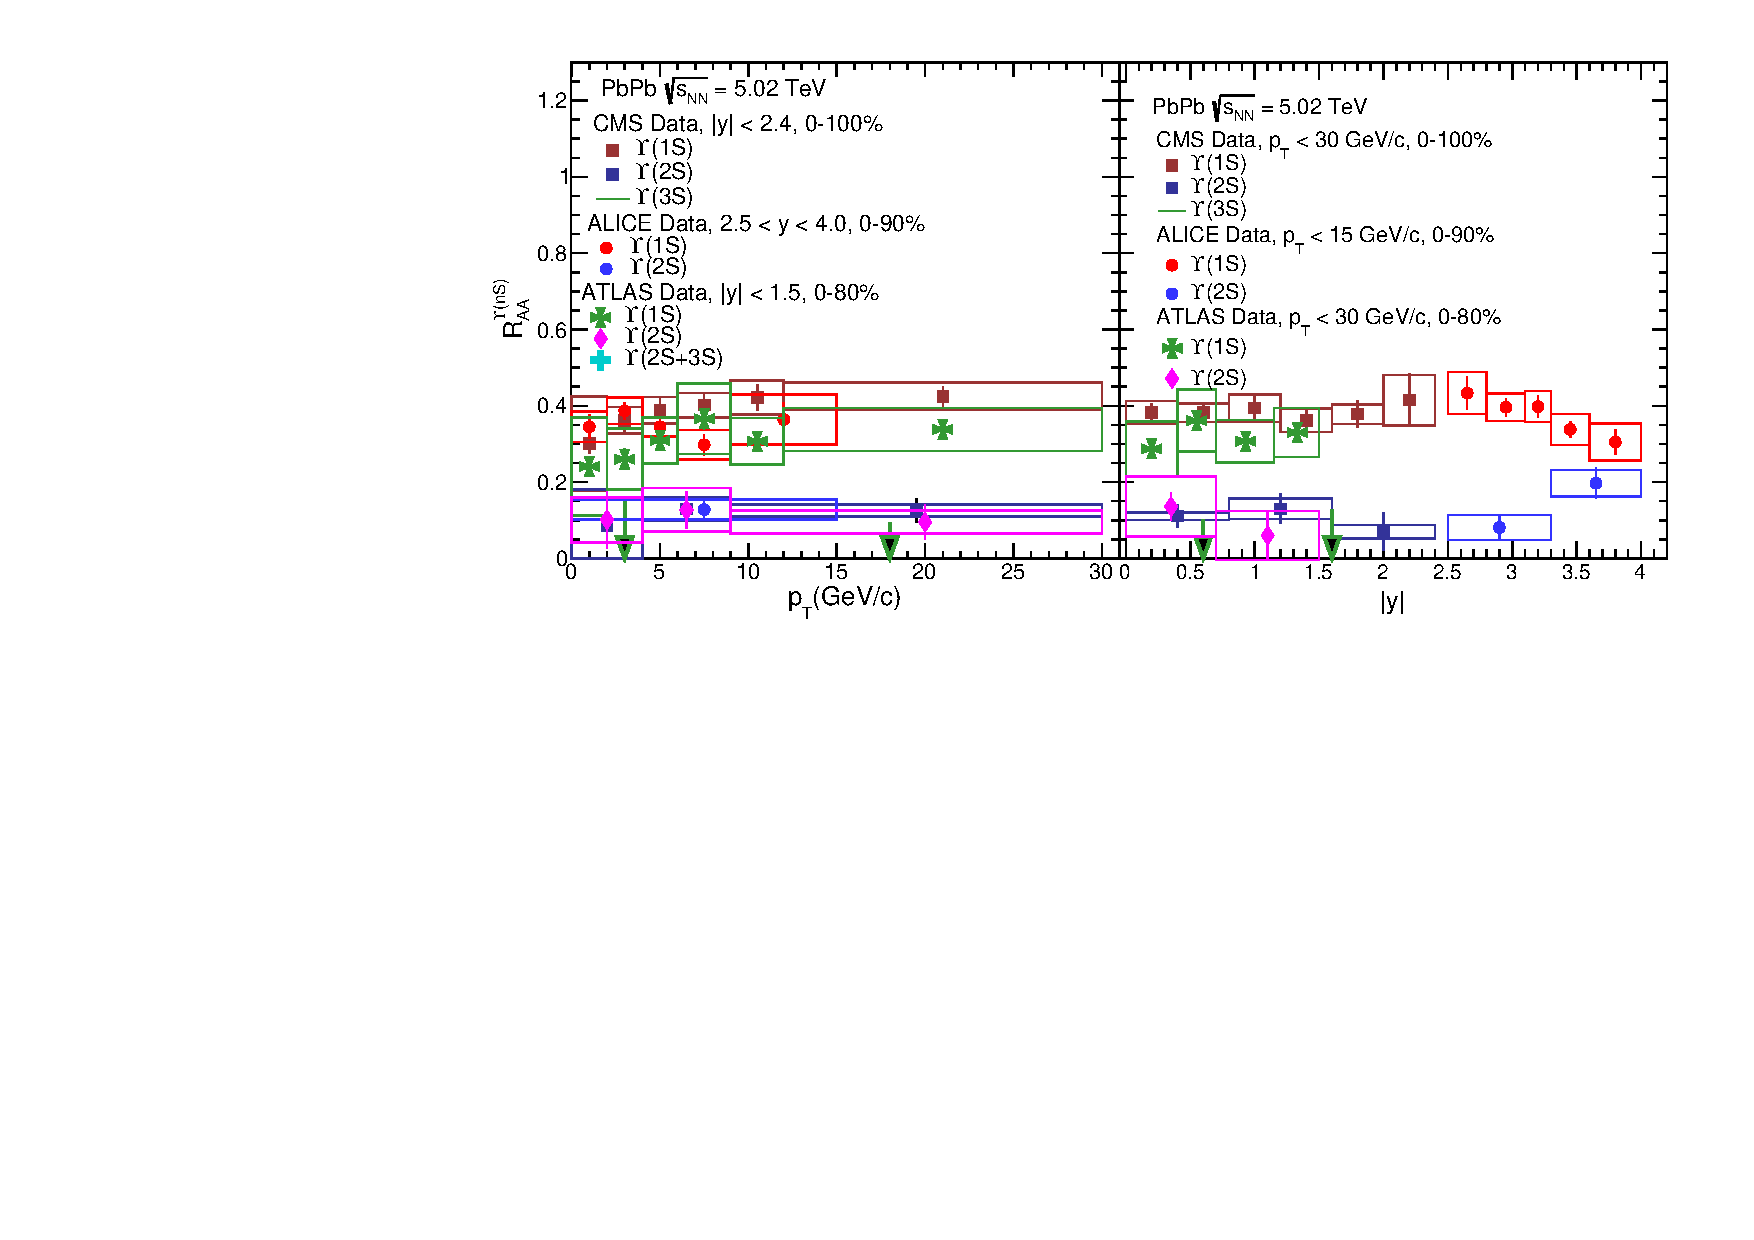
\includegraphics[width=0.99\textwidth]{Figures/ExpOverview/Fig_LHC_YnSRAAPtRap.pdf}
  \caption{(Color online) The $\Upsilon$(nS) nuclear modification factor, $R_{AA}$, (a) as a function of transverse momentum $p_{T}$
    and (b) as a function of rapidity measured by CMS~\cite{CMS:2018zza} and ALICE experiments~\cite{ALICE:2020wwx}. The vertical bars denote statistical uncertainties, and the rectangular boxes show the total systematic uncertainties.
  }
  \label{fig:LHCYnSRAAPtRap}
\end{figure}


\begin{figure}
  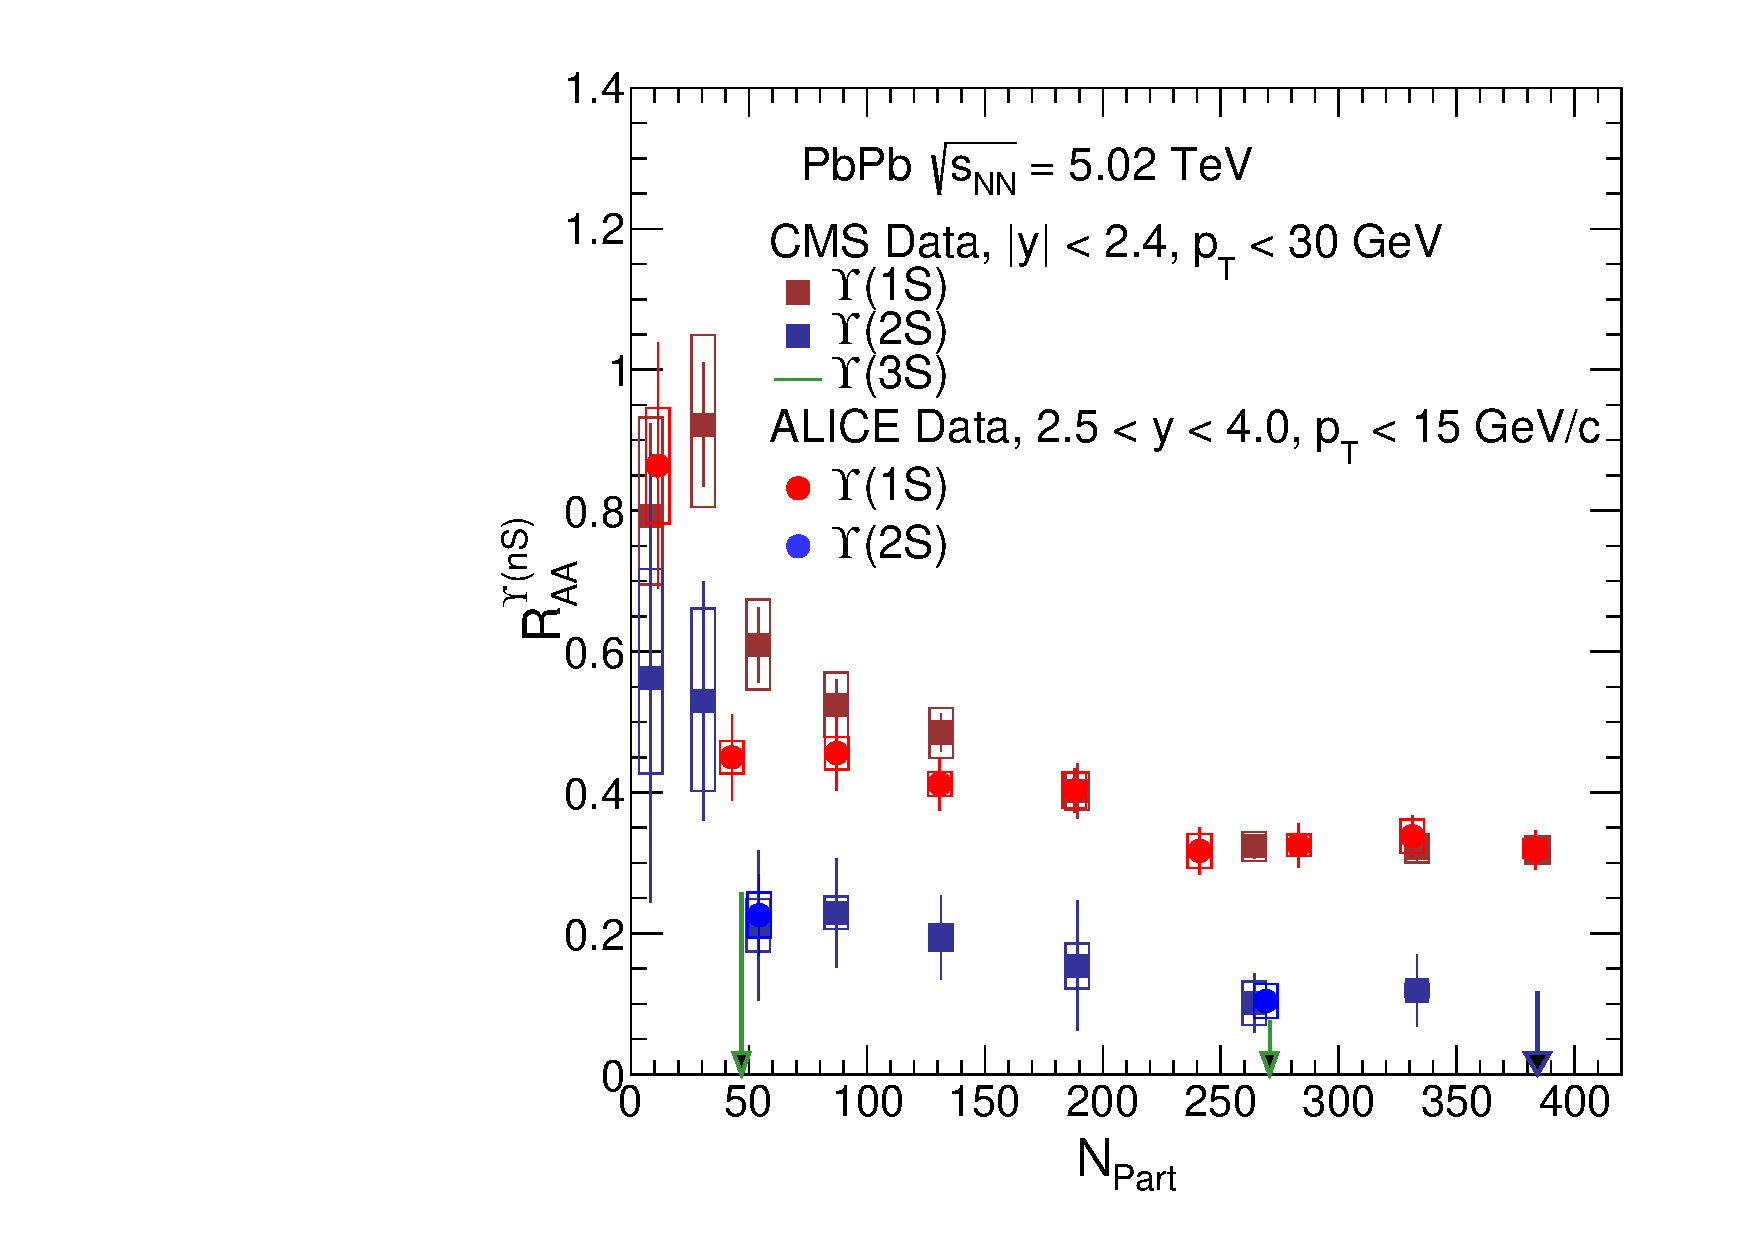
\includegraphics[width=0.49\textwidth]{Figures/ExpOverview/Fig_LHC_YnSRAANPart.pdf}
  %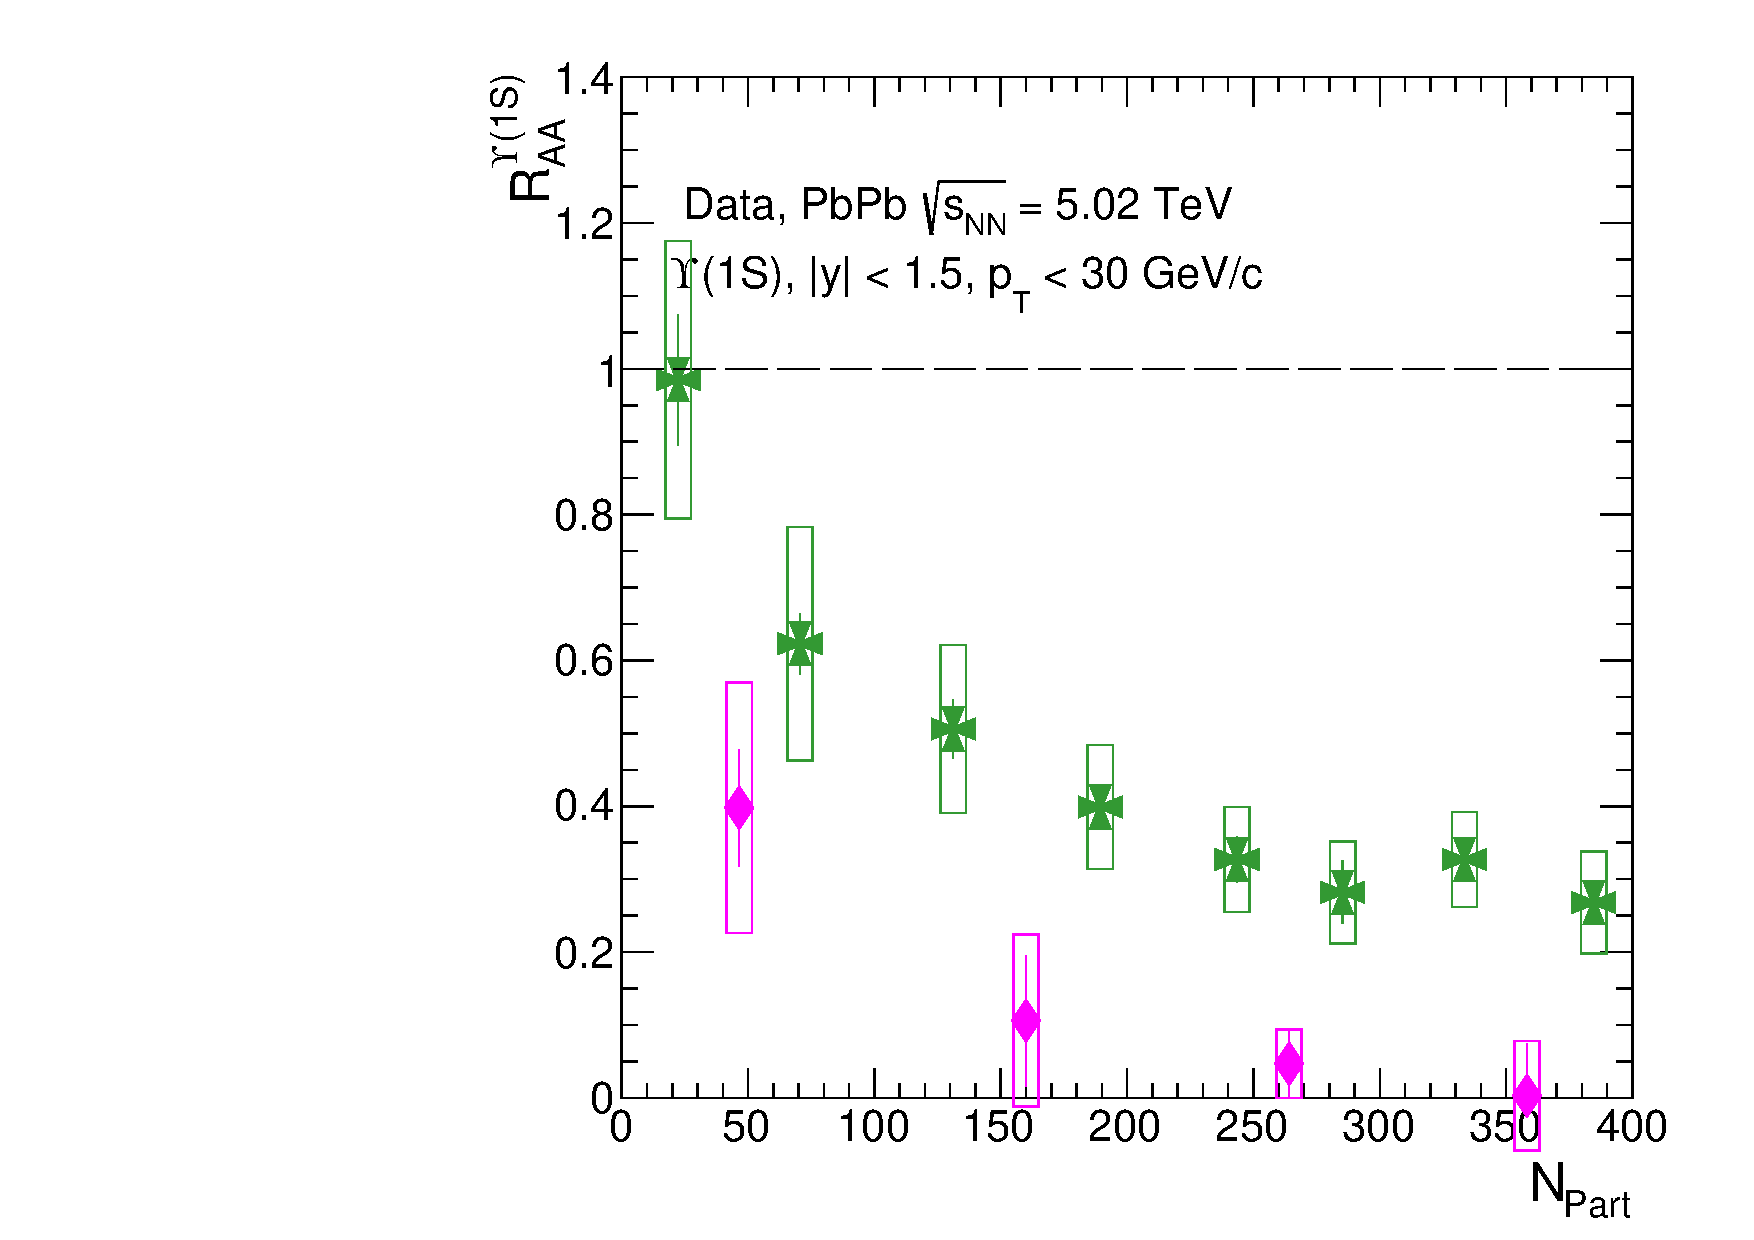
\includegraphics[width=0.49\textwidth]{Figures/ExpOverview/Fig_ATLAS_YnSRAACent_temp.pdf}
  \caption{(Color online) The $\Upsilon$(nS) nuclear modification factor, $R_{AA}$ as a function of N$_{\rm Part}$
    measured by CMS~\cite{CMS:2018zza}, ALICE experiments~\cite{ALICE:2020wwx} and ATLAS experiments~\cite{ALICE:2020wwx}.
    The vertical bars denote statistical uncertainties and the rectangular boxes show the total systematic uncertainties.
  }
  \label{fig:LHCYnSRAANPart}
\end{figure}



\begin{figure}
  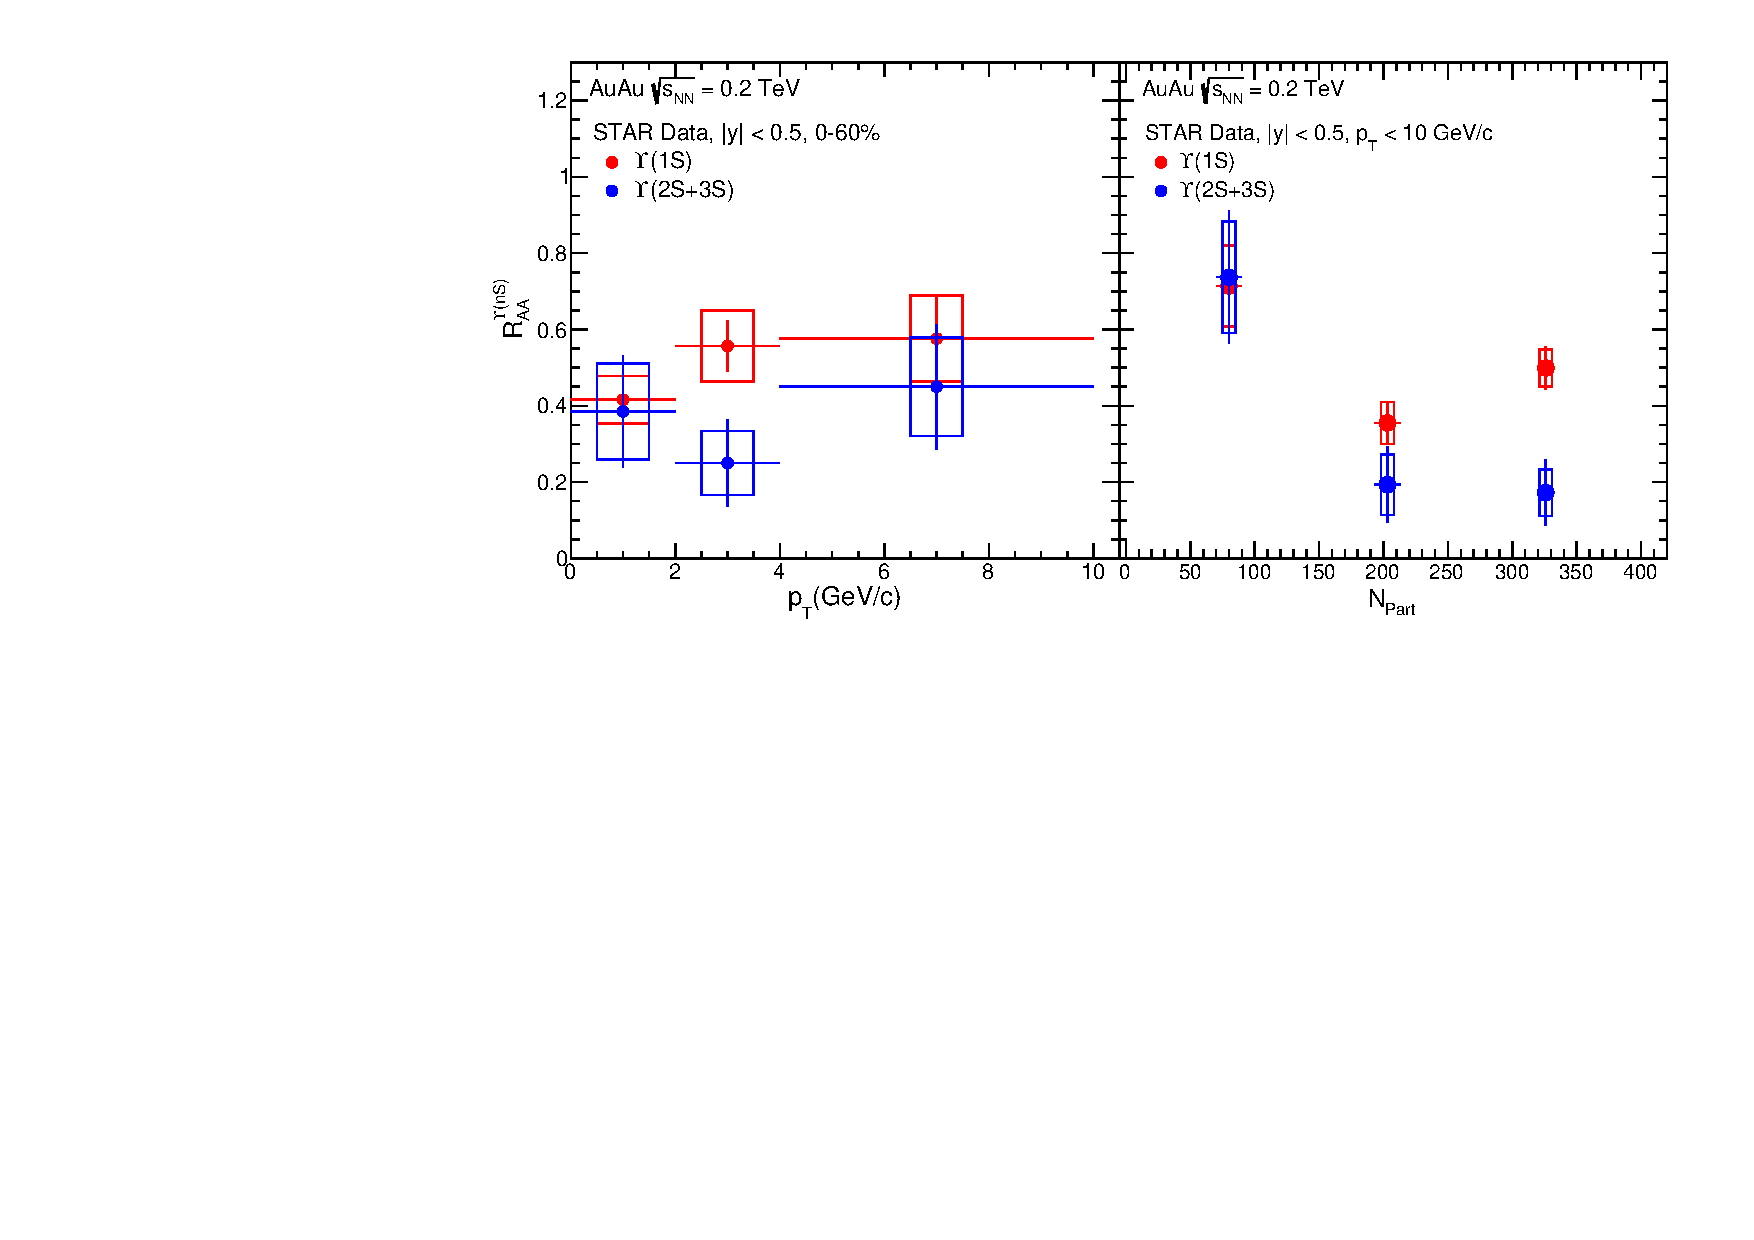
\includegraphics[width=0.99\textwidth]{Figures/ExpOverview/Fig_RHIC_YnSRAAPt.pdf}
  \caption{(Color online) The $\Upsilon$(nS) nuclear modification factor, $R_{AA}$, (a) as a function of transverse momentum $p_{T}$
    and (b) as a function of N$_{\rm Part}$ measured by STAR experiments~\cite{Wang:2019vau}. The vertical bars denote
    statistical uncertainties, and the rectangular boxes show the total systematic uncertainties.
  }
  \label{fig:RHICYnSRAAPtNPart}
\end{figure}



\begin{figure}
  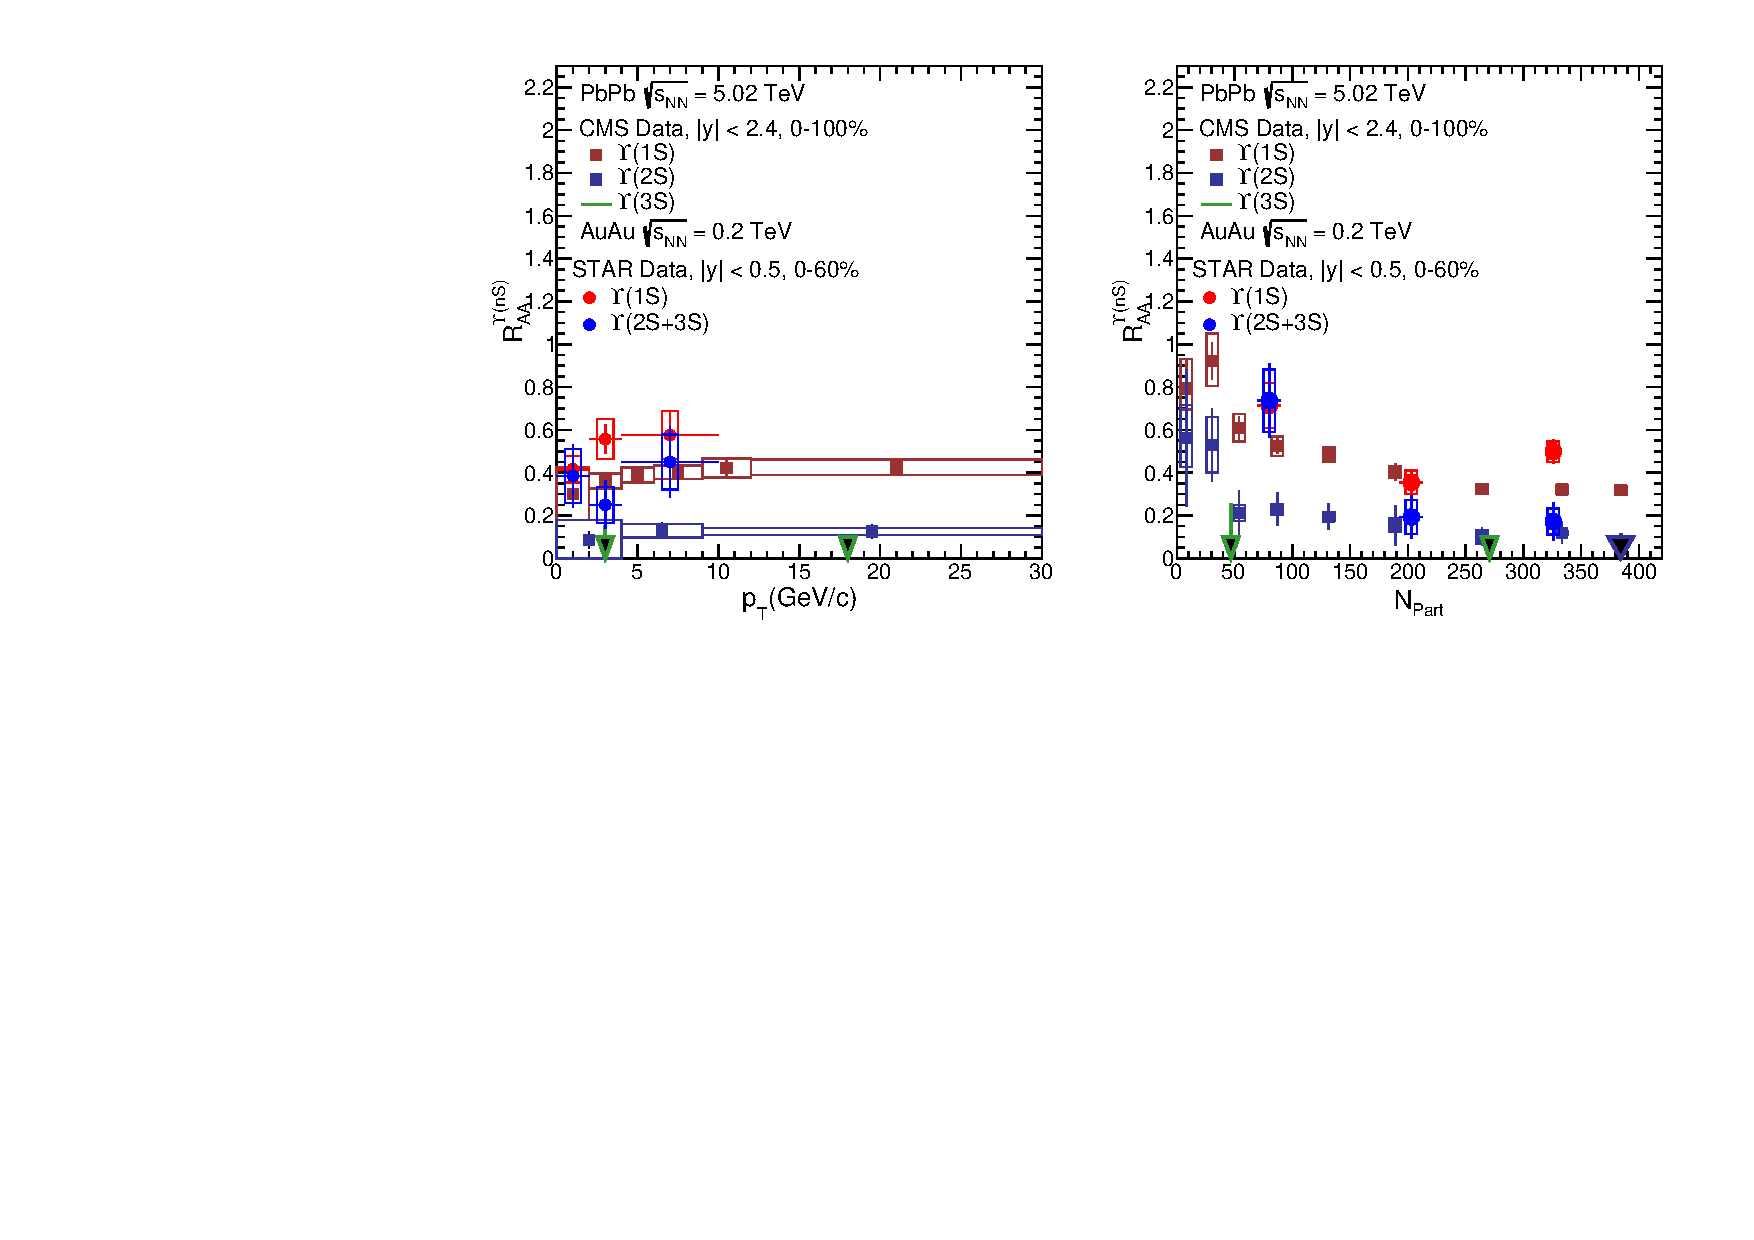
\includegraphics[width=0.99\textwidth]{Figures/ExpOverview/Fig_RHIC_LHC_YnSRAA.pdf}
  \caption{(Color online) The $\Upsilon$(nS) nuclear modification factor, $R_{AA}$, (a) as a function of transverse momentum $p_{T}$
    and (b) as a function of N$_{\rm Part}$ measured by STAR experiments~\cite{Wang:2019vau} at 0.2 TeV and CMS experiment~\cite{CMS:2018zza} at 5.5 TeV.
    The vertical bars denote statistical uncertainties, and the rectangular boxes show the total systematic uncertainties.
  }
  \label{fig:RHICYnSRAAPtNPart}
\end{figure}








\subsection{$\Upsilon$(nS) azimuthal anisotropy}

\begin{figure}
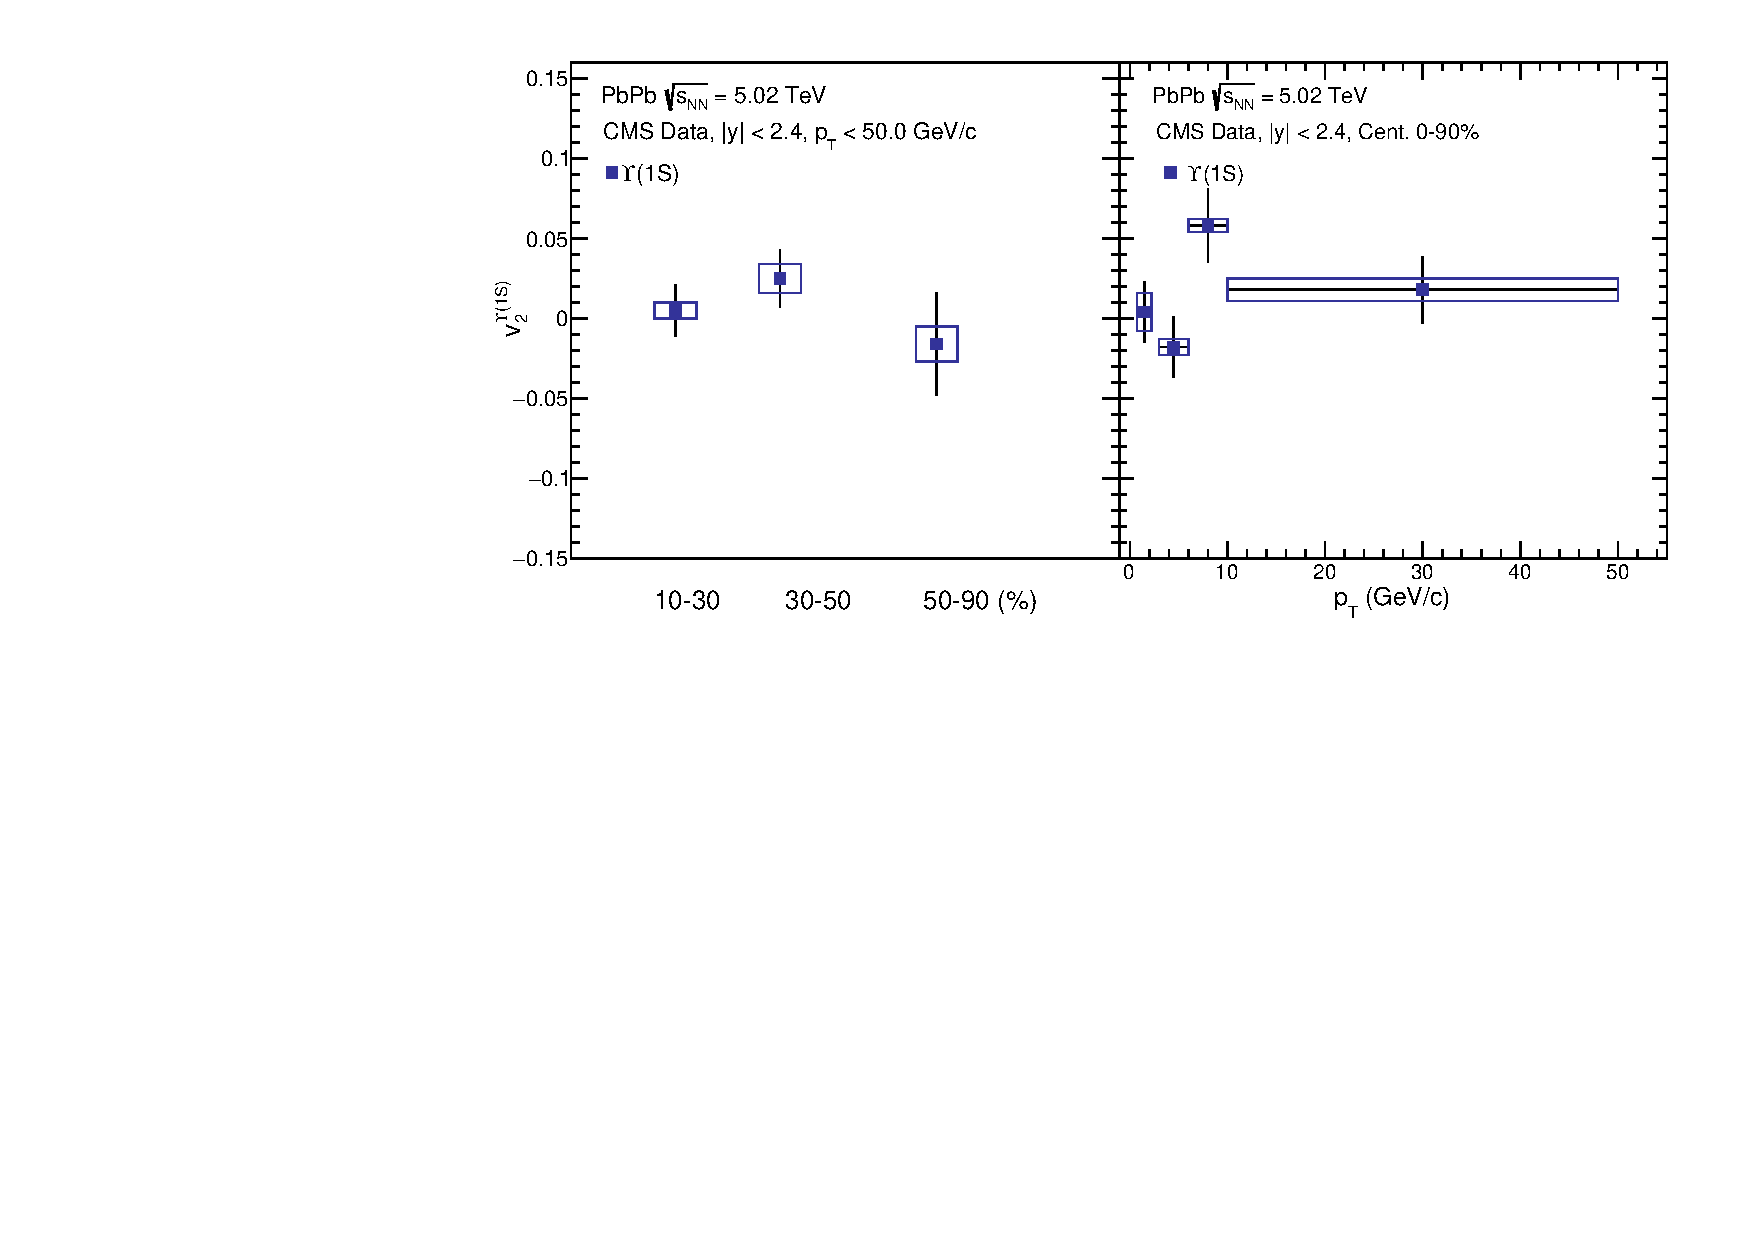
\includegraphics[width=0.99\textwidth]{Figures/ExpOverview/Fig_CMS_Y1S_5TeV_V2.pdf}
\caption{(Color online) The $\Upsilon$(1S) azimuthal anisotropy (v$_{2}$) (a) as a function of collision centrality and 
  (b) as a function of transverse momentum $p_{T}$~\cite{CMS:2020efs}. The vertical bars denote statistical uncertainties,
  and the rectangular boxes show the total systematic uncertainties.
}
\label{fig:Upsilon1SV2CMS}
\end{figure}



The CMS experiment measured v$_{2}$ coefficients for $\Upsilon$(1S) and $\Upsilon$(2S) mesons in PbPb collisions
at a nucleon-nucleon center-of-mass energy of 5.02TeV. Figure~\ref{fig:Upsilon1SV2CMS} shows the $\Upsilon$(1S) azimuthal
anisotropy (v$_{2}$) (a) as a function of collision centrality and (b) as a function of transverse momentum $p_{T}$ measured
by CMS experiment at LHC~\cite{CMS:2020efs}. The p$_{T}$ integrated results
shown in Fig.~\ref{fig:Upsilon1SV2CMS} (a) for three centrality intervals are consistent with zero within the statistical
uncertainties. The average v$_{2}$ values in the 10-90$\%$ centrality interval measured by CMS experiment are found to
be 0.007$\pm$0.011(stat)$\pm$0.005(syst) for $\Upsilon$(1S) and -0.063$\pm$0.085(stat)$\pm$0.037(syst) for $\Upsilon$(2S).   
The p$_{T}$ dependence of $\Upsilon$(1S) meson v$_{2}$ values is measured for the 10-90$\%$ centrality interval.
The v$_{2}$ values are consistent with zero in the measured p$_T$ range, except for the 6$<$p$_{T}<$10 GeV/c interval that
shows a 2.6$\sigma$ deviation from zero. 

\begin{figure}
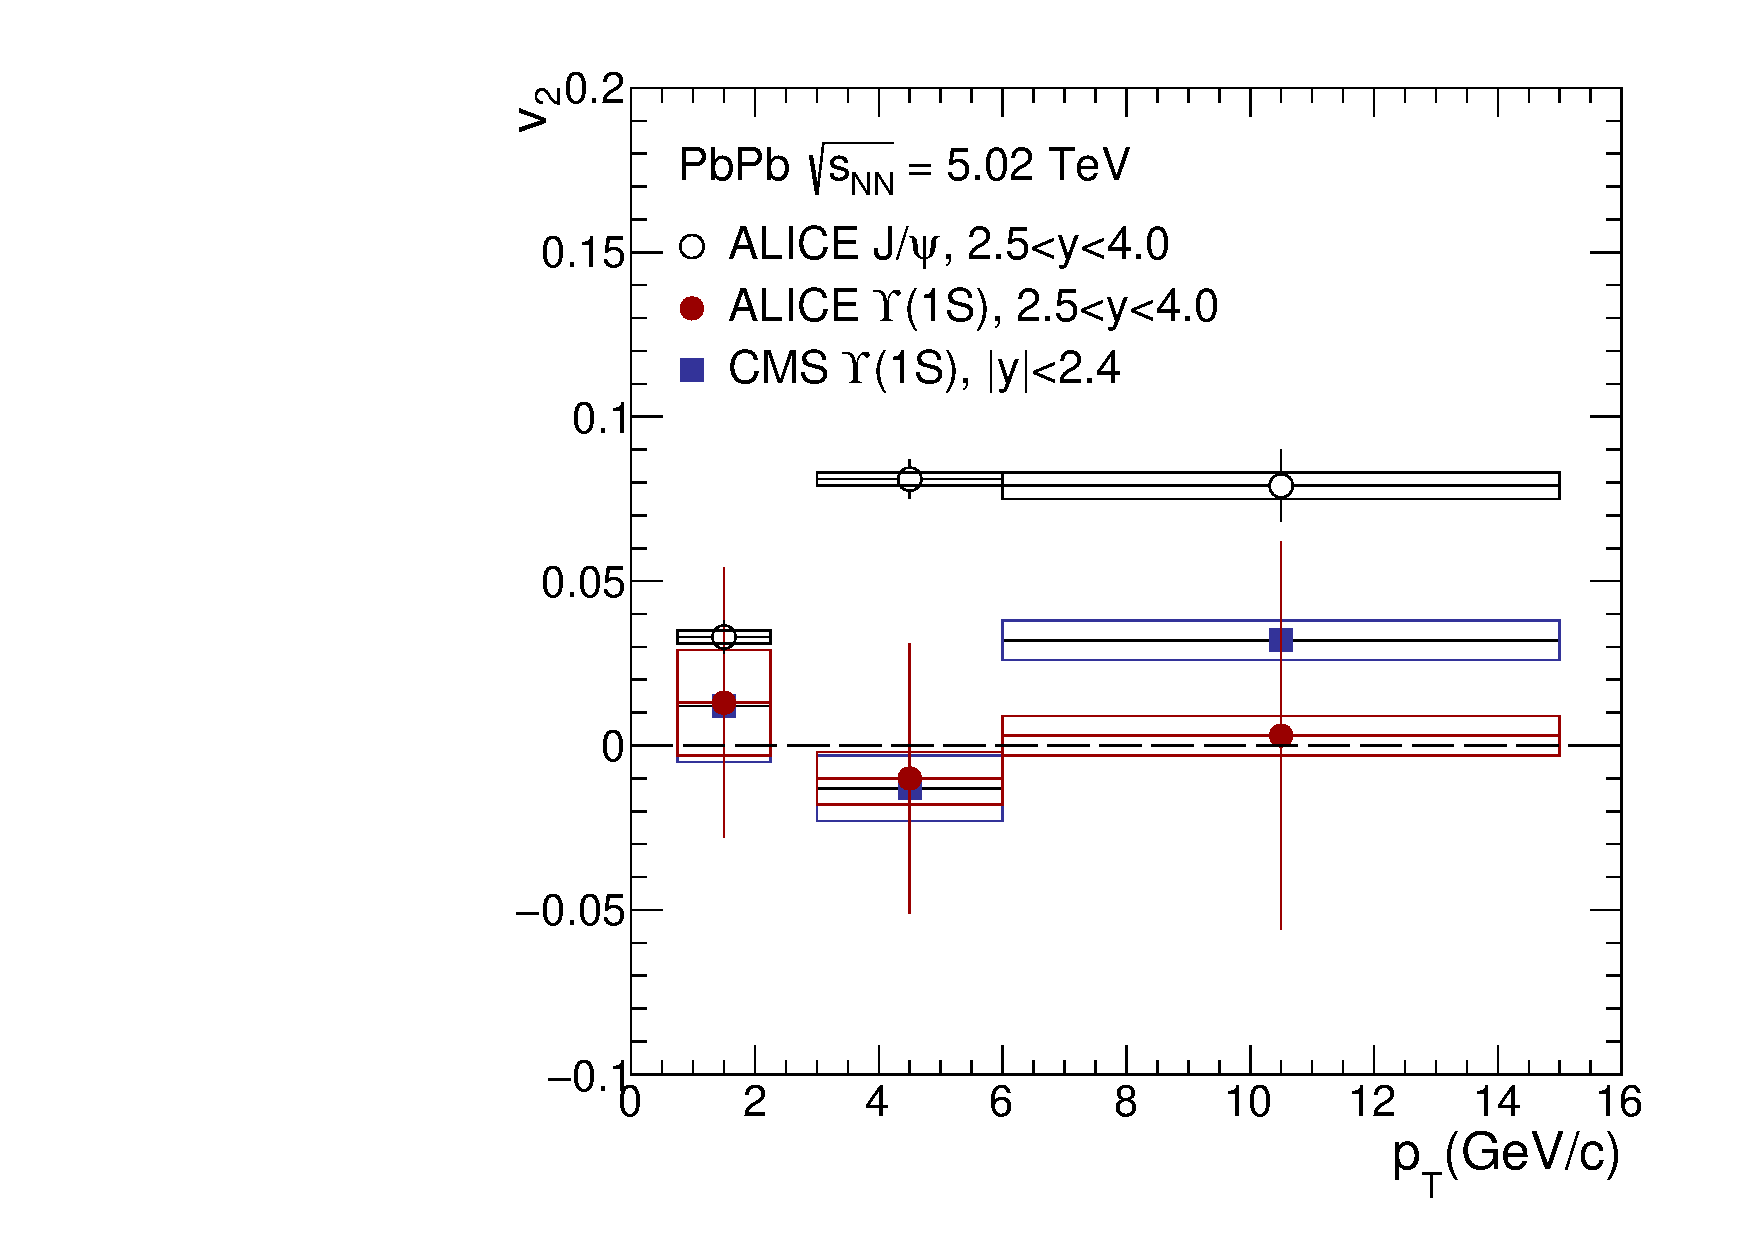
\includegraphics[width=0.49\textwidth]{Figures/ExpOverview/Fig_CMS_ALICE_Y1S_5TeV_V2.pdf}
\caption{(Color online) The v$_{2}$ for $\Upsilon$(1S) mesons as a function of p$_{T}$ in the rapidity range |y|$<$2.4 measured by
  CMS experiment~\cite{CMS:2020efs} compared with the ALICE results for $Upsilon$(1S) and J/$\psi$ mesons measured
  in 2.5$<$y$<$4~\cite{ALICE:2019pox}. The vertical bars denote statistical uncertainties,
  and the rectangular boxes show the total systematic uncertainties.
}
\label{fig:Upsilon1SV2Compare}
\end{figure}

Figure~\ref{fig:Upsilon1SV2Compare} shows the p$_{T}$ differential results for v$_{2}$ of $\Upsilon$(1S)
mesons measured by CMS experiment along with the measurements of v$_{2}$ for $\Upsilon$(1S) and J/$\psi$
from ALICE in the same p$_{T}$ (0-15 GeV/c) and centrality (5-60$\%$) interval. The measurements from CMS
and ALICE are done in complementary rapidity ranges. The $\Upsilon$(1S) V$_{2}$ is consistant with zero while
the J/$\psi$ meson measured by ALICE in same kinematic conditions have finite v$_{2}$. Together, the CMS and ALICE
results indicate that the geometry of the medium has little influence on the $\Upsilon$(1S) yields and recombination is
not a dominant process in the production of this meson. The results also indicate that the path-length depen-dence of
$\Upsilon$(1S) suppression is small.



\subsection{$\Upsilon$(nS) R$_{pA}$ }

\begin{figure}
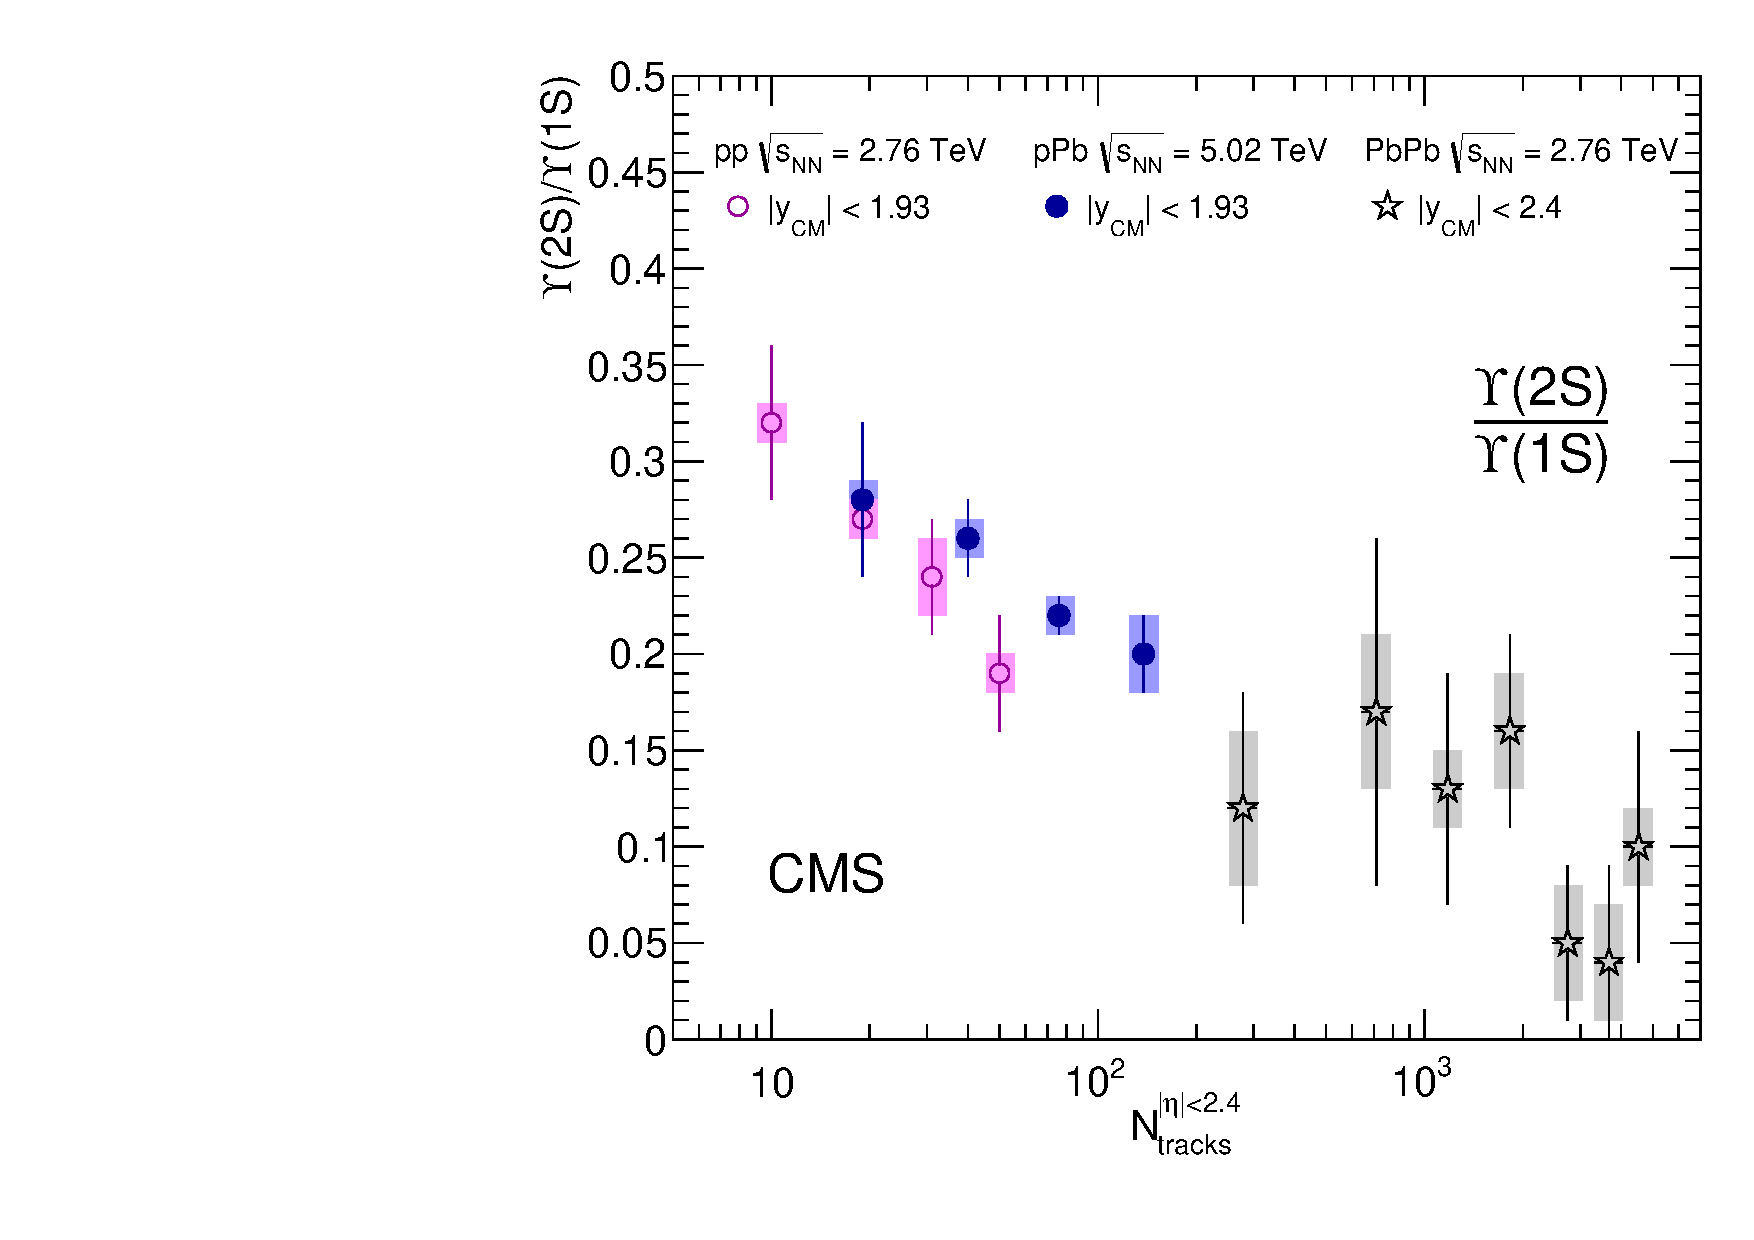
\includegraphics[width=0.49\textwidth]{Figures/ExpOverview/Fig_trk_pPb.pdf}
\caption{(Color online) pPb
}
\label{fig:UpsilonpPb}
\end{figure}

\section{Bottomonia production mechanism in heavy ion collisions}
\label{sec:Bottomonia_hi}

Quarkonia are predicted to be suppressed in heavy ion collisions
if QGP is formed since the force amoung the quarks will be colour screened
in QGP phase~\cite{Matsui:1986dk}.
 However, very soon it was realized that the picture was not that simple.
There are many factors which affect the production of quarkonia in A+A collisions. 
In fact, the quarkonium suppression was observed in proton-nucleus (p+A)
collisions as well.
That part of the nucleus-nucleus suppression is due to 
cold-nuclear-matter (CNM) effects. Therefore it is necessary to disentangle hot 
and cold-medium effects. The CNM effects can arise at the initial
state and/or the final state. The initial state effect
arises due to modification of parton distribution functions (PDF) inside the nucleus
compared to the same inside the protons. The final state modification 
arises due to the  fact the produced quarkonia would interact with the medium
leading to the destabilisation of the bound state. Furthermore, the suppression of
quarkonia is thought to be of sequential in nature.  The sequential suppression
happens as a result of the differences of the  binding energy of different bound states. 
The tightly bound states, such as the $\upsa$ or the $\jpsi$,  melt at higher 
temperatures. On the other hand  more loosely bound staes \psiP, \chic, \chib, 
\upsb or \upsc  melt at much lower temperatures.  This property helps  
 estimating the initial temperature reached in 
the collisions~\cite{Digal:2001ue}. However, the prediction of a sequential 
suppression pattern gets complicated due to feed-down 
decays of higher-mass resonances. The production process is further 
enriched, in the high energy scenario (like LHC), due to recombination process. At very 
high energies, abundant production of $Q$ and $\bar Q$ may lead to new quarkonia production 
in the medium. The recombination process is more justified for charmonia state and 
for the bottommonia states the contribution of this process is expected to be much
smaller since the bottom quark mass ($\sim$ 4.5 GeV) is three times more than the
charm quark and thus its thermalization at temperatures reached at LHC
($\sim$ 0.6 GeV) will be negligible. 



%In the following we discuss different contribution to the medium modification of quarkonia production. 


%\subsubsection{Spectral properties at high temperature}
%\label{sec:media_subsec31}
%There has been considerable interest in studying quarkonia in hot media as it was thought be a signature of the quark-hadron phase transition. 
%since publication of the famous Matsui and Satz 
 %paper~\cite{Matsui:1986dk}.



\subsection{Cold nuclear matter effects}
%{\color{red} This subsection will include the details of the models which use nuclear PDFs for quarkonia production
%like EPS19 or Color Glass Condensate modes. etc.~\cite{}. These effects are small for the Upsilon sector. }

The baseline for quarkonium production and suppression in heavy-ion collisions 
are determined from studies of cold-nuclear-matter (CNM) effects. The name cold matter 
arises because these effects are observed in hadron-nucleus interactions 
where dense matter effects are much more important compared to the hot matter.
The most important CNM affect is due to the modifications of the parton distribution
functions (PDF) in the nucleus compared to that in the nucleon.
It depends mainly on two parameters, 
the momentum fraction of the parton $(x)$ and the scale of the parton-parton 
interaction $(Q^2)$. The nuclear density modified parton distribution
function is known as nPDF and nPDF to PDF ratio,
$R_i(x,Q^2)=f_i^{p \epsilon A} (x, Q^2) /f_i^p  (x, Q^2)$
quantifies the modification due to nuclear effect. 
In the small $x$ regime $(x < 10^{-2})$, this ratio is less than unity
and is referred to as small-x shadowing. At intermediate  $x(\sim 0.1)$
the ratio shows a hump like structure, a phenomenon known as 
anti-shadowing. Around $x\approx 0.6$, one observes a dip which is known as EMC
effect. The dynamics of partons 
within the nuclei is affected by the parton saturation which is successfully
studied by the color glass condensate. In the 
final state, the quarkonia bound state scatters and re-scatters inelastically
while passing through the nucleus. This leads to 
the breakup or absorption of the bound state which is estimated by the
inelastic cross-section of the quarkonia with the nucleon. 

The contributions to CNM effects look straightforward. However there are a several 
uncertainties associated with them. 
The nuclear modifications of the quark densities are relatively 
well-understood as they can be measured in  nuclear deep-inelastic scattering (nDIS).
On the other hand the modifications of the gluon density are not directly measured.
The scaling violations in nDIS is one of the  
ways to constrain the nuclear gluon density. Another constraint is provided by 
overall momentum conservation.  However, more direct probes of the gluon 
density are needed. The shadowing parametrizations we have in hand are derived
from global fits to the nuclear parton densities.
This gives wide variations in the nuclear gluon 
density, from almost no effect to very large shadowing at low-$x$, 
compensated by strong antishadowing around $x \sim 0.1$.  


The nuclear absorption survival probability depends on the absorption cross section 
of the quarkonium. There are more inherent uncertainties 
in absorption than in the shadowing parametrization.
Typically an absorption cross section is a fit to the $A$ dependence 
of quarkonium production in pA collision at a given energy. 
This is rather simplistic since it is not known whether the object traversing the
nucleus is a precursor 
color-octet state or a fully-formed color-singlet quarkonium state.
The \jpsi absorption cross section at $y \sim 0$ is observed to decrease with energy,
irrespective which shadowing parametrizations ar chosen~\cite{Lourenco:2008sk}. 

The analyses of $\jpsi$ production in fixed-target interactions~\cite{Lourenco:2008sk} 
show that the effective absorption
cross section depends on the energy of the initial beam and the rapidity or
$x_F$ of the observed $\jpsi$.  One possible interpretation is that 
low-momentum color-singlet states can hadronize in the
target, resulting in larger effective absorption cross sections at lower
center-of-mass energies and backward $x_F$ (or center-of-mass rapidity).
At higher energies, the states traverse the target more rapidly so that
the $x_F$ values at which they can hadronize in the target move 
back from midrapidity toward more negative $x_F$.
Finally, at sufficiently high energies, the quarkonium states pass 
through the target before hadronizing, resulting in negligible absorption
effects.  Thus the {\it effective} absorption cross section decreases with 
increasing center-of-mass energy.

This is a very simplistic picture. In practice, cold-nuclear-matter effects 
(initial-state energy loss, shadowing, final-state breakup, {\it etc.}) 
depend differently on the quarkonium kinematic variables and the collision energy. 
Thus combining all these mechanisms into an {\it effective} absorption cross section,
as employed in the Glauber formalism is not adequate.
A better understanding of absorption requires more detailed knowledge of the 
production mechanisms which are not fully understood yet.


The nuclear modification factors and ratios of Upsilon states are measured by CMS
experiment covering wide kinematic regions.
In section~\ref{sectionpA}, Figure~\ref{fig:LHCpPb5} shows the $\Upsilon$(nS) nuclear
modification factor, $R_{pA}$,  as a function of transverse momentum $p_{T}$ 
and rapidity in p+Pb colisions at 5.02 TeV measured by CMS~\cite{CMS:2022wfi}.
It is observed that all three Upsilon states are suppressed in p+Pb collisions.
Moreover, it is noticed that the excited states are more suppressed as compared
to the ground state.
Since the shadowing effects are expected to be similar
on all the three states~\cite{Vogt:2015uba}
the measurements indicate final state effects on the Upsilon states which need
to be understood. 


\subsection{Quarkonium in hot medium}
\label{sec:media_sec3}

It has been argued that the color screening 
in a deconfined QCD medium will destroy $\QQbar$ bound states
at sufficiently high temperatures. If the binding radius of the heavy
quark bound state is  much greater than the screening radius, then one heavy 
quark gets screened from the other and the pair is broken~\cite{Abdulsalam:2012bw}.
As the temperature 
increases, the screening radius becomes smaller and smaller compared to the 
binding radius and the quarkonium states become more and more unstable. 
Although, this idea was proposed long ago, first principle QCD calculations, 
which go beyond qualitative arguments, have been performed quite recently. 
Such calculations include lattice QCD determinations of quarkonium 
correlators~\cite{Umeda:2002vr,Asakawa:2003re,Datta:2003ww,Jakovac:2006sf,Aarts:2007pk},
potential model calculations 
of the quarkonium spectral functions with potentials based on lattice 
QCD~\cite{Digal:2001ue,Wong:2004zr,Mocsy:2005qw,Mocsy:2004bv,Alberico:2006vw,Cabrera:2006wh,Mocsy:2007yj,Mocsy:2007jz},
also effective field theory
approaches~\cite{Laine:2007qy,Laine:2007gj,Laine:2008cf,Brambilla:2008cx}.  
Furthermore, better modeling of 
quarkonium production in the medium created by heavy-ion collisions has 
been achieved. These new advancements improve the understanding of 
the hot-medium effects on the quarkonium states which is crucial for the 
interpretation of heavy-ion data. 



\begin{figure}[h]
   \begin{center}
      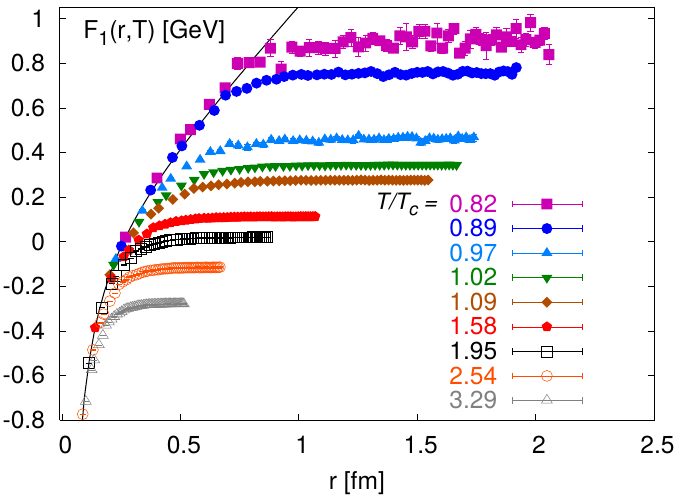
\includegraphics[width=0.6\textwidth]{Figures/Fig16_LattSingEnergy.png}
      \caption{(Color online) The singlet free energy as a function of quark separation 
        calculated in (2+1) flavour QCD on $16^3 \times 4$ lattices at different 
             temperatures~\cite{Petreczky:2009ip,Petreczky:2010yn}.  
      }
      \label{Fig:LatticeSingEner}
   \end{center}
\end{figure}
In Lattice Gauge Theory, color screening is studied  by 
calculating the spatial correlation function of a static quark and
antiquark in a color-singlet state which propagates in Euclidean time 
from $\tau=0$ to $\tau=1/T$, where $T$ is the temperature.
The result of such calculations on the Lattice  with dynamical quarks have been
reported in Refs.~\cite{Petreczky:2009ip,Petreczky:2010yn,Kaczmarek:2002mc}.
The logarithm of the singlet correlation function, also called the singlet free energy,
is shown for (2+1) flavour in Fig.~\ref{Fig:LatticeSingEner} for
different temperatures.
As expected, in the zero-temperature limit,
the singlet free energy coincides with the zero-temperature potential. 
Also at sufficiently short distances, the singlet free energy is
temperature independent which is given by the zero-temperature potential. 
The range of interaction is shown to decrease with increasing temperature.
For temperatures just above the transition temperature, $T_c$, the heavy-quark 
interaction range becomes comparable to the charmonium radius. Based on 
this observation, it can be expected that the charmonium
states, as well as the excited bottomonium states, do not remain bound at
temperatures just above the deconfinement transition, often referred to as 
dissociation or melting. 

%\subsubsection{Quarkonium spectral functions and quarkonium potential}
%\label{sec:media_subsec33}
In-medium quarkonium properties are encoded in the corresponding 
spectral functions, such as quarkonium dissociation
at high temperatures. Spectral functions are defined as
the imaginary part of the retarded correlation function of quarkonium
operators where the bound states appear as peaks.
The peaks broaden and eventually disappear with increasing temperature which
signals the melting of the given quarkonium state.
The quarkonium spectral functions can be calculated in potential models 
using the singlet free energy from Fig.~\ref{Fig:LatticeSingEner} or with different 
lattice-based potentials obtained using the singlet free energy
as an input~\cite{Mocsy:2007yj,Mocsy:2007jz}. 
The results for quenched QCD calculations
for S-wave charmonium  and bottomonium spectral functions~\cite{Mocsy:2007yj}
are shown in Fig.~\ref{Fig:QuarkoniaSpecFuncLattice}.
It shows that all charmonia states are dissolved in the deconfined phase above $T_c$ while the
bottomonium 1S state may persist up to $T \sim 2T_c$. An upper bound on the dissociation
temperature above which no bound state peaks can be seen in the spectral function can be
obtained from the analysis of the spectral functions.
Conservative upper limits on the dissociation temperatures for the different quarkonium
states obtained from  a full QCD calculation~\cite{Mocsy:2007jz} are given in
Table~\ref{tab:LatticeDissTemp}.

\begin{figure}[]
   \begin{center}
      {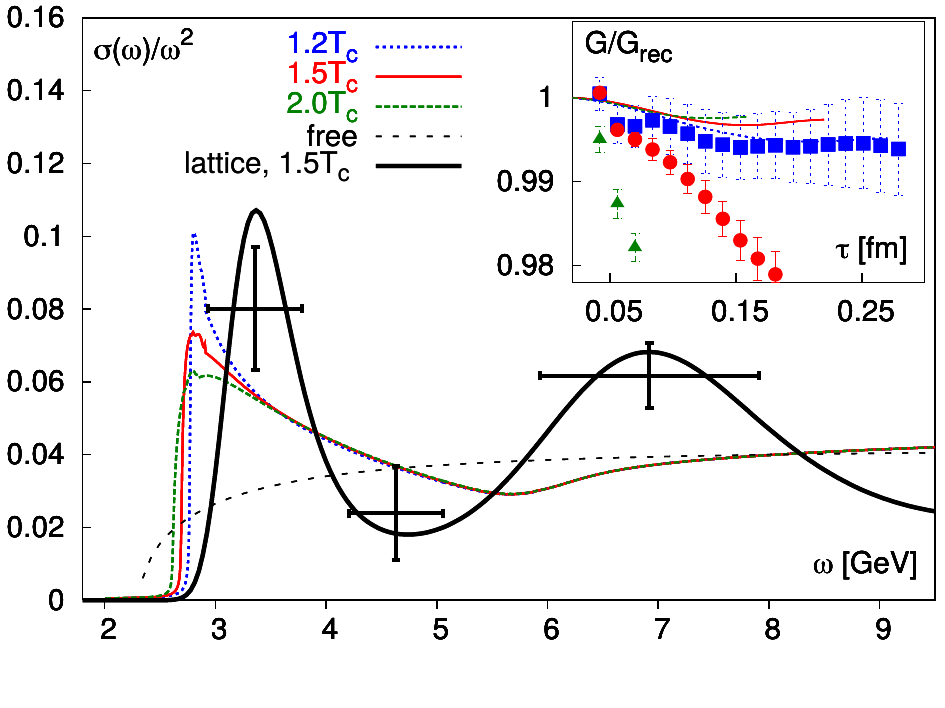
\includegraphics[width=0.49\textwidth]{Figures/Fig17l_JPsi_SpecFuncLattQCD.png}}
      {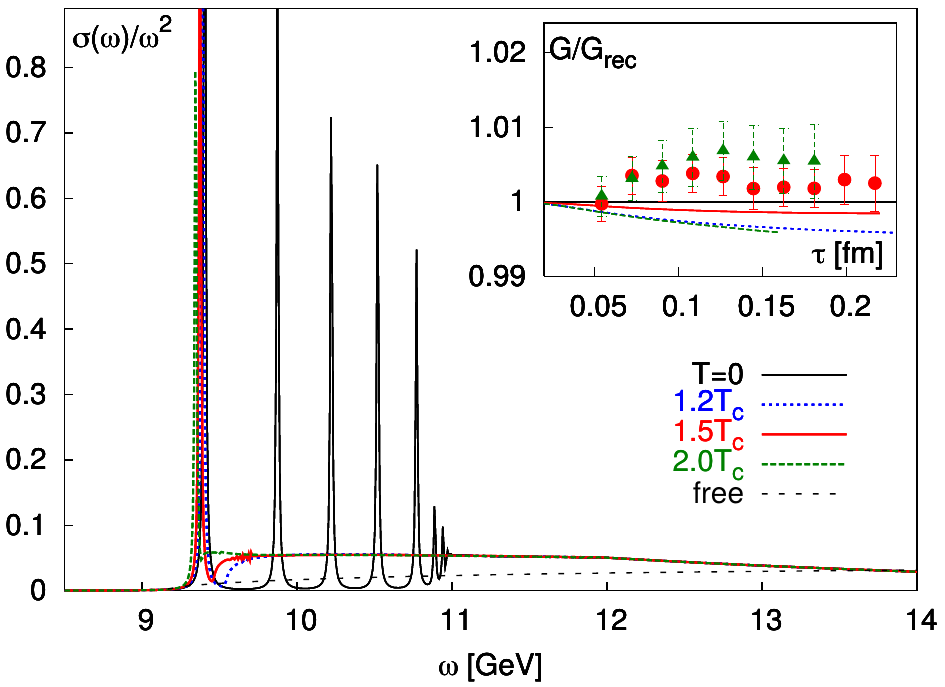
\includegraphics[width=0.49\textwidth]{Figures/Fig17r_Y1S_SpecFuncLattQCD.png}}
      \caption{(Color online) The S-wave charmonium (left) and 
        bottomonium (right) spectral functions calculated in potential 
        models. 
        Insets give correlators compared to lattice data.  
        The {\it dotted curves} are the
        free spectral functions. Figures are taken from Ref.~\cite{Mocsy:2007yj}.
      }
      \label{Fig:QuarkoniaSpecFuncLattice} 
   \end{center}
\end{figure}





\begin{table}[tb]
   \caption{Upper bounds on the dissociation 
             temperatures for different quarkonia states~\cite{Mocsy:2007jz}.
             }
   \label{tab:LatticeDissTemp}
   \setlength{\tabcolsep}{0.41pc}
   \begin{center}
      \begin{tabular}{ccccccc}
      \hline\hline
      %\rule[10pt]{-1mm}{0mm}
      State & $\chi_{cJ}(1P)$ & $\psi^{'}$ &J/$\psi$  &$\Upsilon(2S)$ & $\chi_{bJ}(1P)$ &$\Upsilon(1S)$ \\%[1.0mm]
      \hline 
      %\rule[10pt]{-1mm}{0mm}
      $T_{\rm diss}$ & $\le T_c$ & $\le T_c$ & $1.2T_c$ & $1.2T_c$ & $1.3T_c$ & $2T_c$\\ 
\hline\hline
\end{tabular}
\end{center}
\end{table}



%\subsubsection{Summary of hot medium effects}
%\label{sec:SummMedEff}
Potential model calculations based on lattice QCD and resummed 
perturbative QCD calculations conclude that all charmonium states and the
excited bottomonium states dissolve in the deconfined medium.
This can account  
for the reduction of the quarkonium yields in heavy-ion collisions 
compared to the p+p collisions scaled by number of binary collisions.
Recombination and edge effects, however, will produce a nonzero yield.


              
\subsection{Bottomonia suppression using Lattice QCD inspired potential model rates}

Bottomonia suppression has been studied using first-principle
calculation of the thermal widths of the states and considering 
momentum anisotropy of the plasma~\cite{Strickland:2011aa,Krouppa:2016jcl,Krouppa:2018lkt}.
In this work, the phase-space distribution of gluons in the local
rest frame is taken to be 

\begin{equation} 
f({\bf x},{\bf p}) = f_{\rm iso}\left(\sqrt{{\bf p}^2+ \xi({\bf p}\cdot{\bf n})^2 }  / 
p_{\rm hard} \right).
\label{distribution}
\end{equation} 
In the above equation, $\xi$ is a measure of the degree of anisotropy of the plasma given as 
%\begin{equation}
$\xi = \frac{1}{2} \langle 
{\bf p}_\perp^2\rangle/\langle p_z^2\rangle -1$
%\end{equation} 
where $p_z$ and 
${\bf p}_\perp $ are the partonic longitudinal and transverse momenta in the local
rest frame, respectively. In equation \ref{distribution}, $p_{\rm hard}$ is the momentum  
scale of the particles and can be identified with the temperature
in an isotropic plasma. 

An approximate form of the real perturbative heavy quark potential as a function of
$\xi$ can be written as~\cite{Dumitru:2007hy} (for $N_c=3$ and $N_f=2$). 
\begin{eqnarray}
Re[V_{\rm pert}] &=& - \alpha \exp(-\mu r)/r, \nonumber \\
\left(\frac{\mu}{m_D}\right)^{-4} &=&  
1 + \xi\left(1 + \frac{\sqrt{2}(1+\xi)^2\left(\cos(2\theta) - 1 \right)}{(2+ \xi)^{5/2}} \right),
\label{eq:muparam}
\end{eqnarray}
where $\alpha = 4\alpha_s/3$ and $m_D^2 = (1.4)^2 16 \pi \alpha_s  \, p_{\rm hard}^2/3$ gives
the isotropic Debye mass and $\theta$ is the angle with respect to the beamline.  
The factor of $(1.4)^2$ accounts for higher-order corrections to the isotropic Debye 
mass \cite{Kaczmarek:2004gv}.

This perturbative potential, given in equation (\ref{eq:muparam}) is modified to include
the non-perturbative (long range) contributions. 
The modified real part of the potential is given as~\cite{Dumitru:2007hy} 


%
\begin{equation} 
\label{eq:repot}
Re[V] = -\frac{\alpha}{r} \left(1+\mu \, r\right) \exp\left( -\mu
\, r  \right) + \frac{2\sigma}{\mu}\left[1-\exp\left( -\mu
\, r  \right)\right] 
 - \sigma \,r\, \exp(-\mu\,r)- \frac{0.8 \, \sigma}{m_Q^2\, r} \, ,
\end{equation}
%
where the last term is a temperature- and spin-independent quark mass correction 
\cite{Bali:1997am} and $\sigma = 0.223$ GeV is the string tension.  Here  $\alpha$ 
is chosen to be  $0.385$ 
to match zero temperature
binding energy data for heavy quark states \cite{Dumitru:2007hy}.
The imaginary part of the potential is taken same as the perturbative heavy quark
potential up to linear order in $\xi$ 
%
\begin{equation} 
Im[V_{\rm pert}] = -\alpha p_{\rm hard} \biggl\{ \phi(\hat{r}) - \xi \left[\psi_1(\hat{r},
\theta)+\psi_2(\hat{r}, \theta)\right]\biggr\} ,
\label{eq:impot}
\end{equation}
%
where $\hat{r}=m_D r$ and $\phi$, $\psi_1$, and $\psi_2$ are defined in Ref.~\cite{Krouppa:2016jcl}. 

 The full model potential, given by $V = Re[V] + i Im[V]$, is used to 
solve the Schr\"odinger equation. 
Solution of the Schr\"odinger equation gives the real and imaginary parts of 
the binding energy of the states.  The imaginary part defines the instantaneous width of the state
$Im[E_{\rm bind}(p_{\rm hard},\xi)] \equiv -\Gamma_T(p_{\rm hard},\xi)/2$. 
The resulting width $\Gamma_T(\tau)$ implicitly depends on the initial temperature of the
system.

The following rate equation is used to account for in-medium bottomonia state decay,
%
\begin{equation} \label{eq:rate}
\frac{dn(\tau,{\bf x}_\perp,\varsigma)}{d\tau} = -\Gamma(\tau,{\bf x}_\perp,\varsigma)n(\tau,{\bf x}_\perp,\varsigma) ,
\end{equation}
%
where   $\tau = \sqrt{t^{2} - z^{2}}$ is the longitudinal proper time,  ${\bf x}_{\perp}$ is the the transverse coordinate and 
 $\varsigma = {\rm arctanh}(z/t)$ is the the spatial rapidity. The rate of decay is computed by~\cite{Strickland:2011aa}
%
\begin{eqnarray}
\Gamma(\tau, {\bf x}_{\perp}, \varsigma) = 
& 2Im[E_{\text{bind}}(\tau, {\bf x}_{\perp}, \varsigma)] & \ \ Re[E_{\text{bind}}(\tau, {\bf x}_{\perp}, \varsigma)] > 0 \\ 
& = \gamma_{\text{dis}} & \ \ Re[E_{\text{bind}}(\tau, {\bf x}_{\perp}, \varsigma)] \leq 0. 
%\end{cases}
\end{eqnarray}
%
The suppression factor $R_{AA}$ as a function of $p_T$ and centrality 
is obtained as follows
\begin{equation}
R_{AA}({\bf x}_\perp,p_T,\varsigma,b) =% 
\exp\!\left(-\bar{\gamma}({\bf x}_\perp,p_T,\varsigma,b) \right),
\end{equation}
where
\begin{equation}
 \bar{\gamma}({\bf x}_\perp,p_T,
\varsigma,b) \equiv \Theta(\tau_f-\tau_{\rm form}(p_T)) \int_{{\rm max}(\tau_{\rm form}(p_T),\tau_0)}^{\tau_f} 
d\tau\,\Gamma_T(\tau,{\bf x}_\perp,\varsigma,b).
\end{equation}
  Here $\tau_{0}$ and $\tau_{f}$ are the initial and freeze out times of the plasma and 
$\tau_{\rm form}$ is the formation time of the bottomonium state. 
Finally, one averages
over ${\bf x}_\perp$ to obtain 
\begin{equation}
\langle R_{AA}(p_T,\varsigma,b) \rangle \equiv 
\frac{\int_{{\bf x}_\perp} \! d{\bf x}_\perp \, T_{AA}({\bf x}_\perp)\,%
  R_{AA}({\bf x}_\perp,p_T,\varsigma,b)} 
{\int_{{\bf x}_\perp} \! d{\bf x}_\perp \, T_{AA}({\bf x}_\perp)}.
\end{equation} 

\begin{figure}[t]
\begin{center}
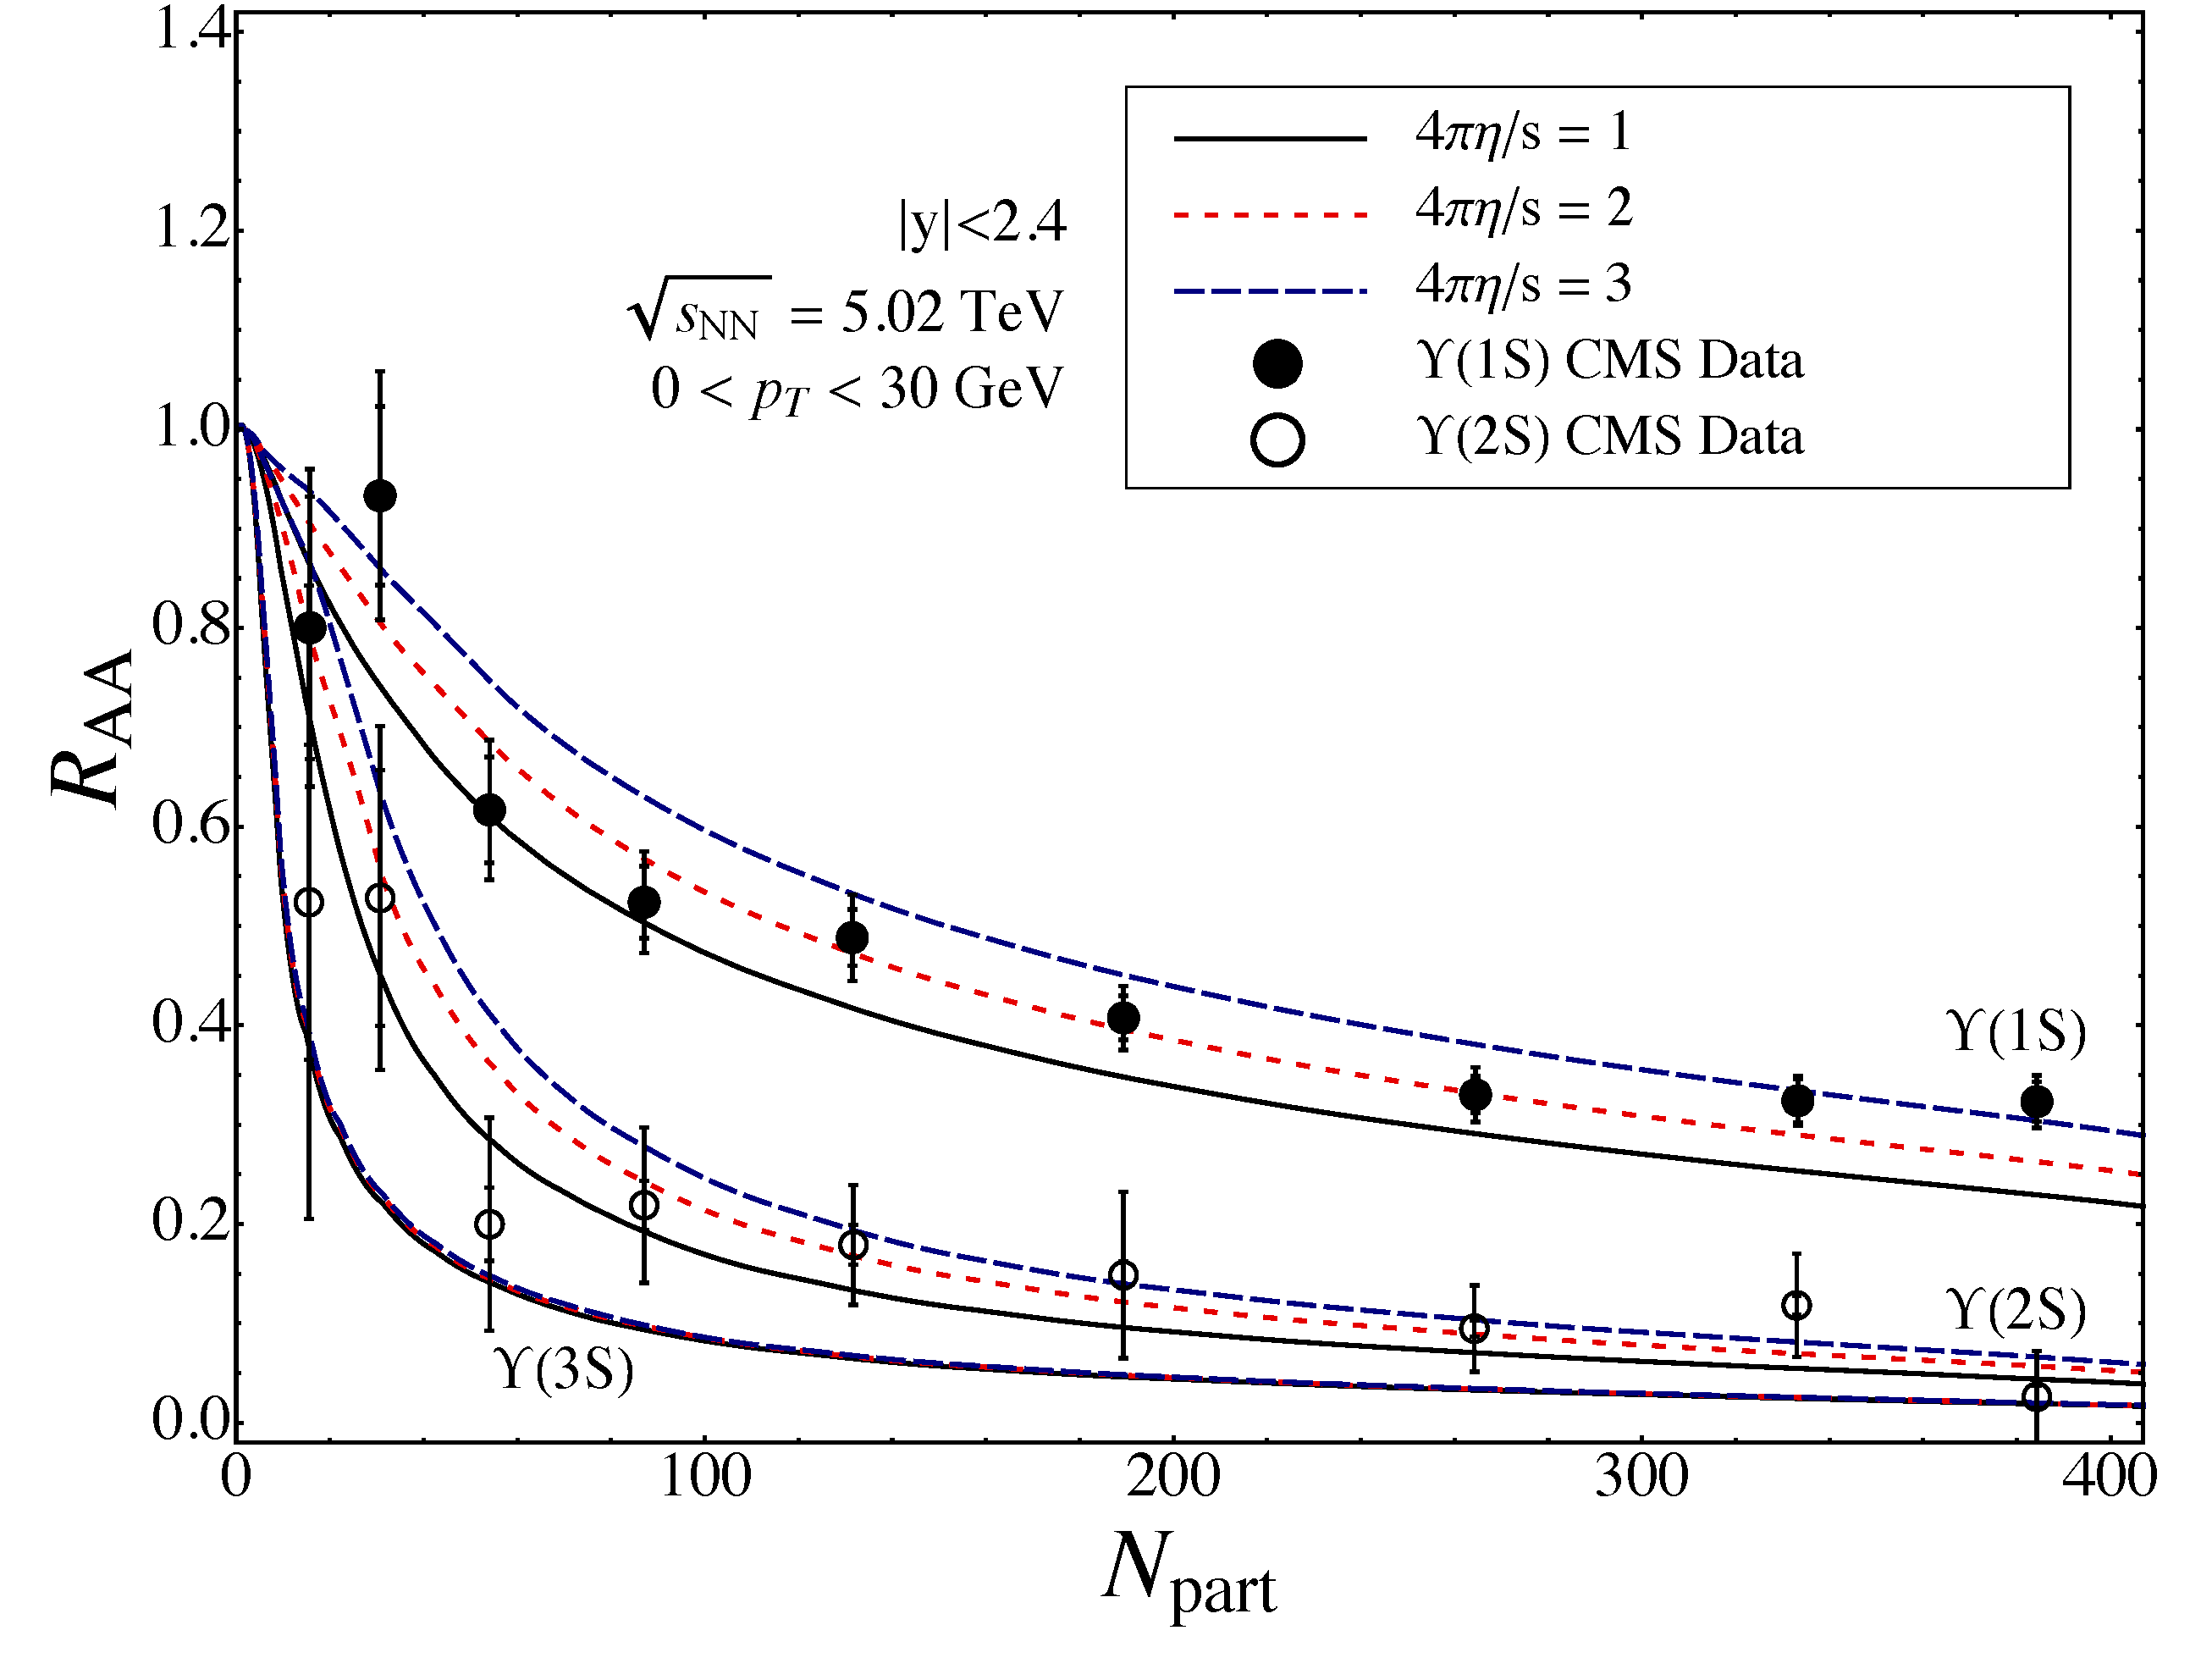
\includegraphics[width=0.5\textwidth]{Figures/Fig18_YnsRAA_NPart_StricklandModel.pdf}
\end{center}
\vspace{-7mm}
\caption{(Color online) Model calculations \cite{Krouppa:2018lkt} of the $R_{\rm AA}$
  of $\Upsilon$(1S) and $\Upsilon$(2S) as a function of $N_{\text{part}}$
  in Pb+Pb collisions at $\sqrt{s_{\rm NN}}$=5.02 TeV.   
  A comparison is made with the data from CMS experiment \cite{CMS:2018zza} at
  the LHC.}
\label{fig:raasep}
\end{figure}

Figure~\ref{fig:raasep} shows the model calculations~\cite{Krouppa:2018lkt}
of the $R_{\rm AA}$ of $\Upsilon$(1S) and $\Upsilon$(2S) as a function of
$N_{\text{part}}$  in Pb+Pb collisions at $\sqrt{s_{\rm NN}}$=5.02 TeV.   
  A comparison is made with the data from CMS experiment \cite{CMS:2018zza} at
  the LHC. It is shown that there is substantial 
suppression  of $\Upsilon(1S)$ and $\Upsilon$(2S) which are attributed to the in-medium decay.  
A  similar suppression pattern is observed for $\chi_{b1}$ which 
may be attributed to the finite formation time of the $\chi_{b1}$. 
  


\subsection{Gluon dissociation of quarkonia in dynamical medium}

{\color{black}
  The quarkonia can undergo both dissociation and recombination during the
  evolution of medium.
 The evolution of quarkonia population $N_{Q}$ with proper time $\tau$ can be studied via
a kinetic equation~\cite{Thews:2000rj}
  \begin{equation}\label{eqkin}
    {dN_{Q} \over d\tau}  =  - \lambda_D  \rho_g N_{Q} + \lambda_F {N_{q \bar{q}}^{2} \over V(\tau)},
  \end{equation}
  where $V(\tau)$ is the volume of the deconfined spatial region.
  The $\lambda_{D}$ is the dissociation rate obtained by the dissociation cross section
averaged over the momentum distribution of gluons $\rho_g$ and $\lambda_{F}$ is the formation
rate obtained by the formation cross section 
averaged over the momentum distribution of heavy quark pair $q$ and $\bar{q}$. 
$N_{q \bar{q}}$ is the number of initial heavy quark pairs produced per event which depends
on the centrality defined by the number of participants.
  The number of quarkonia at freeze-out time $\tau_f$ is given by the solution of Eq.~(\ref{eqkin}),
  \begin{equation}
    N_{Q}(p_T) = S(p_T) \,N_{Q}^{\rm PbPb}(p_T)+N_{Q}^F(p_T).
    \label{eqbeta}
  \end{equation}
  Here $N_{Q}^{\rm PbPb}(p_T)$ is the number of initially-produced quarkonia (including shadowing)
  as a function of $p_T$ and $S(p_T)$ is their survival probability from gluon collisions at
  freeze-out given by 
  \begin{equation}
    S(p_T) = \exp \left( {-\int_{\tau_0}^{\tau_f}f(\tau) \lambda_{\rm D}(T,p_T)\,\rho_g(T)\,d\tau} \right).
  \end{equation}
  The temperature $T(\tau)$ and the QGP fraction $f(\tau)$ evolve from initial time $\tau_0$ 
  to freeze-out time $\tau_f$ due to expansion of the QGP. The initial temperature and the 
  evolution is dependent on collision centrality $N_{\rm part}$.
  $N_{Q}^F(p_T)$ is the number of regenerated quarkonia per event,
  \begin{equation}
    N_{Q}^F(p_T)=S(p_T)N_{q \bar{q}}^{2} \int_{\tau_0}^{\tau_f}{{\lambda_{\mathrm{F}}(T,p_T) \over V(\tau)\,S(\tau,p_T)} d\tau}.
  \end{equation}
  The nuclear modification factor ($R_{AA}$) then can simply be written as~\cite{Kumar:2014kfa, Kumar:2019xdj}
  \begin{equation}
    R_{AA}(p_T)=S(p_T) \, R(p_T) + \frac{N_{Q}^F(p_T)}{N_{Q}^{pp}(p_T)}.
    \label{raa}
  \end{equation}
  Here $R(p_T)$ is the shadowing factor.
%  $R_{AA}$ as a function of collision centrality, including regeneration, is
%  \begin{equation}
%    R_{AA}(N_{\rm part}) = \frac{\int_{p_{T\,\rm cut}} N_{Q}^{pp}(p_T)S(p_T)\, R(p_T) dp_T}{\int_{p_{T\,\rm cut}} N_{Q}^{pp}(p_T) dp_T} + 
%    \frac{\int_{p_{T\, \rm cut}} N_{Q}^F(p_T) dp_T}{\int_{p_{T\, \rm cut}} N_{Q}^{pp}(p_T) dp_T}
%    \label{raa2}
%  \end{equation}
%  Here $p_{T~{\rm cut}}$ defines the $p_T$ range for a given experimental acceptance.
%  $N_{Q}^{pp}(p_T)$ is the unmodified $p_T$ distribution of quarkonia obtained by NLO 
%  calculations and scaled to a particular centrality of the Pb+Pb collisions.

  The gluon dissociation rate can be obtained in the color dipole
approximation~\cite{Bhanot:1979vb} as a function of gluon energy, $q^0$ as
 \begin{equation}
    \sigma_{D}(q^{0}) = {8\pi \over 3} \, {16^2 \over 3^2} {a_0 \over m_q}  \frac{(q^0/\epsilon_0 - 1)^{3/2}} {(q^0/\epsilon_0)^5},
 \end{equation}
  where $\epsilon_0$ is the quarkonia binding energy and $m_q$ is the charm/bottom quark mass 
  and $a_0=1/\sqrt{m_q\epsilon_0}$.
  The value of $\epsilon_0$ is equal to $1.10$ GeV for $\Upsilon$(1S) \cite{Karsch:1987pv}. 
For the first excited state of bottomonia, $\Upsilon$(2S), dissociation
 cross section is given in Ref.~\cite{Arleo:2001mp}.

  \begin{figure}
    \begin{center}
    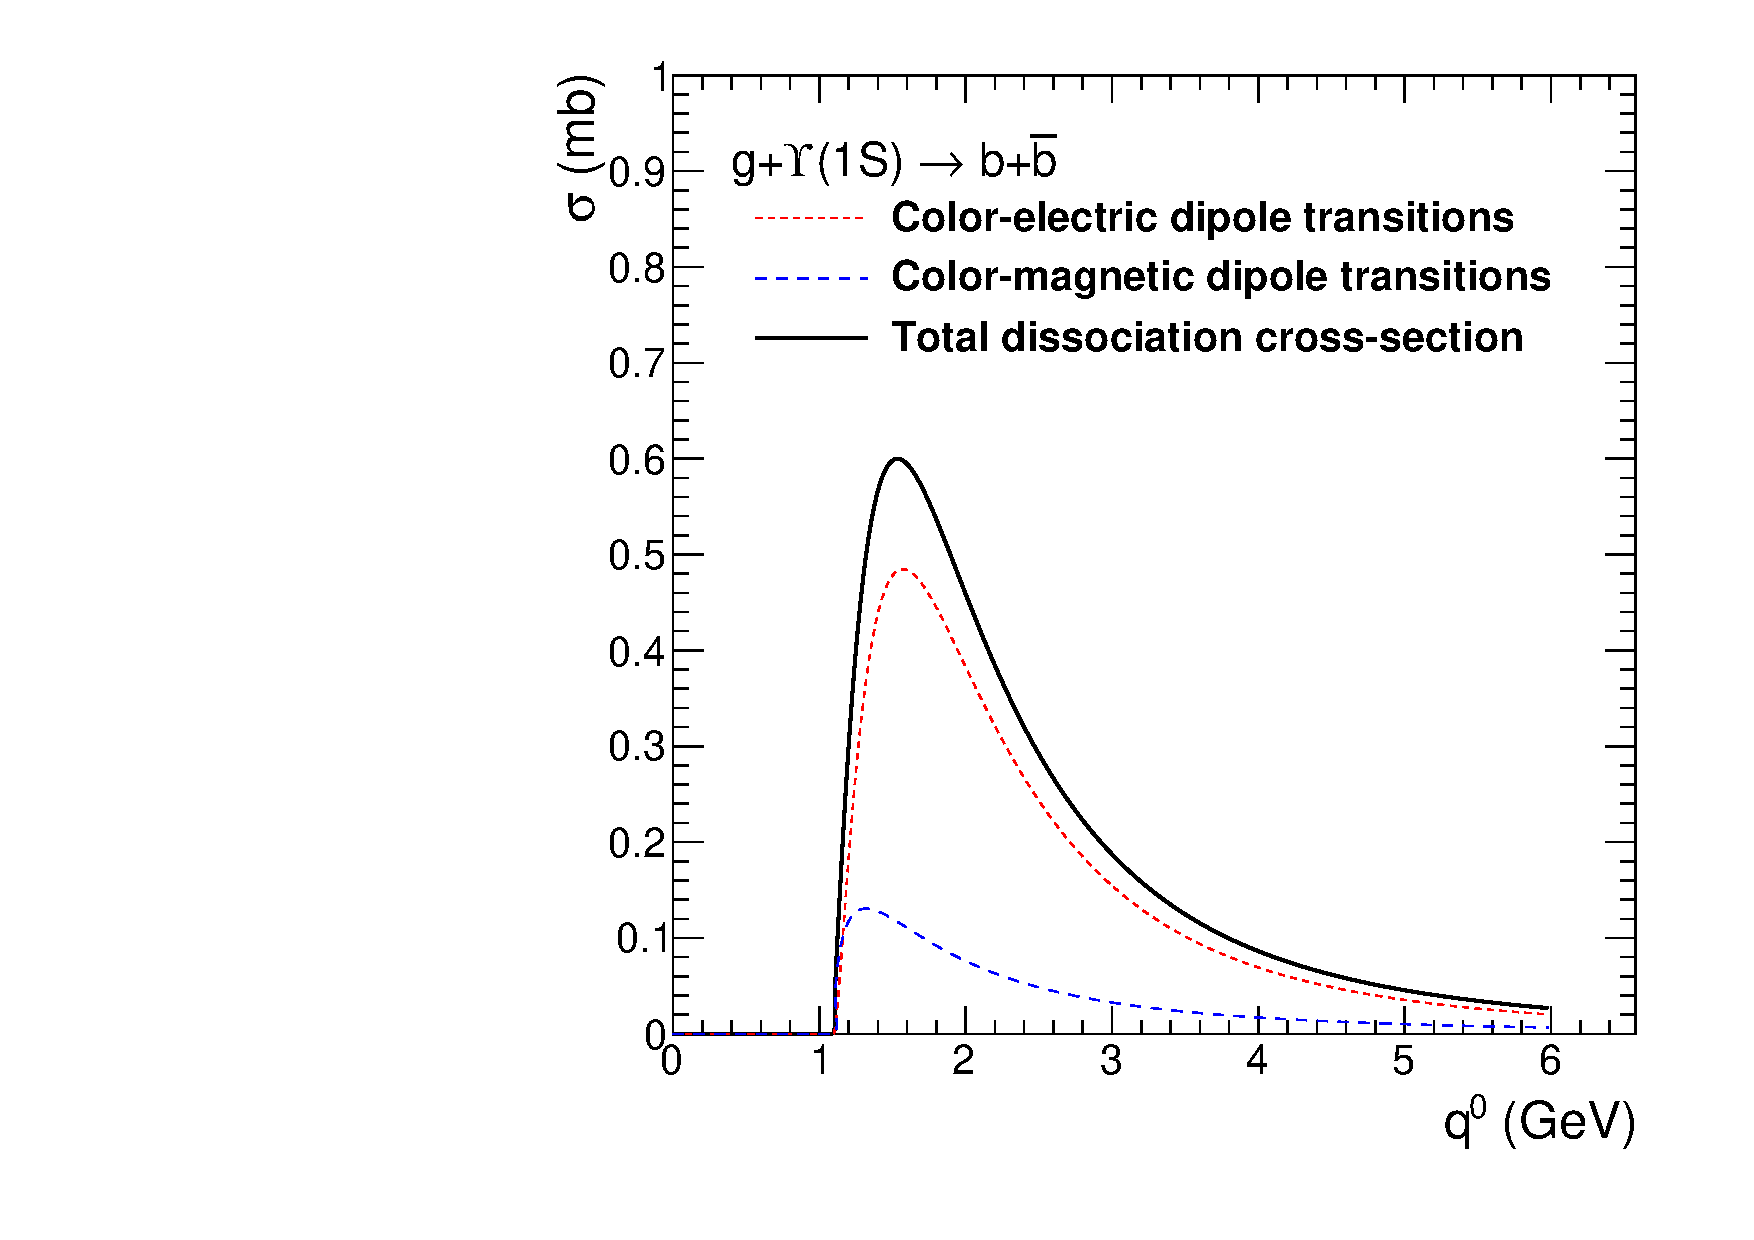
\includegraphics[width=0.50\textwidth]{Figures/Fig19_Y1S_SigmaDq0.pdf}
    \caption{(Color online) Gluon dissociation cross section of $\Upsilon$(1S) as a
      function of gluon energy ($q^{0}$) in $\Upsilon$(1S) rest frame.}
    \label{fig:SigmaDQ0}
    \end{center}
  \end{figure}

  
  Figure \ref{fig:SigmaDQ0} shows the gluon dissociation cross sections of
$\Upsilon$(1S) as a function of gluon energy. The dissociation cross section
is zero when the gluon energy is less than the binding energy of the quarkonia.
It increases with gluon energy and reaches a maximum at 1.5 GeV for 
$\Upsilon(1{\rm S})$. At higher gluon energies, the interaction
probability decreases. The dissociation rate as a function of quarkonium
momentum can be obtained by integrating the dissociation cross section over thermal gluon momentum 
distribution.


 The formation cross section can be obtained from the dissociation cross section using
detailed balance~\cite{Thews:2000rj,Thews:2005vj},
  \begin{equation}
    \sigma_{F} = \frac{48}{36}\,\sigma_{D}(q^0)\frac{(s-M_{Q}^2)^{2}}{s(s-4m_q^{2})}.
  \end{equation}
  The formation rate of quarkonium with momentum {\bf p} can be obtained using
  thermal distribution functions of  $q/\bar{q}$.
  
  

%%%%%%%%%%%%%%%%%%%%%%%%%%%%%%%%%%%%%%%%%%%%%%%%%%%%%%%% 5.02 TeV %%%%%%%%%%%%%%%%%%%%%%%%%%%%%%%%%%%%%%%%%
\begin{figure}
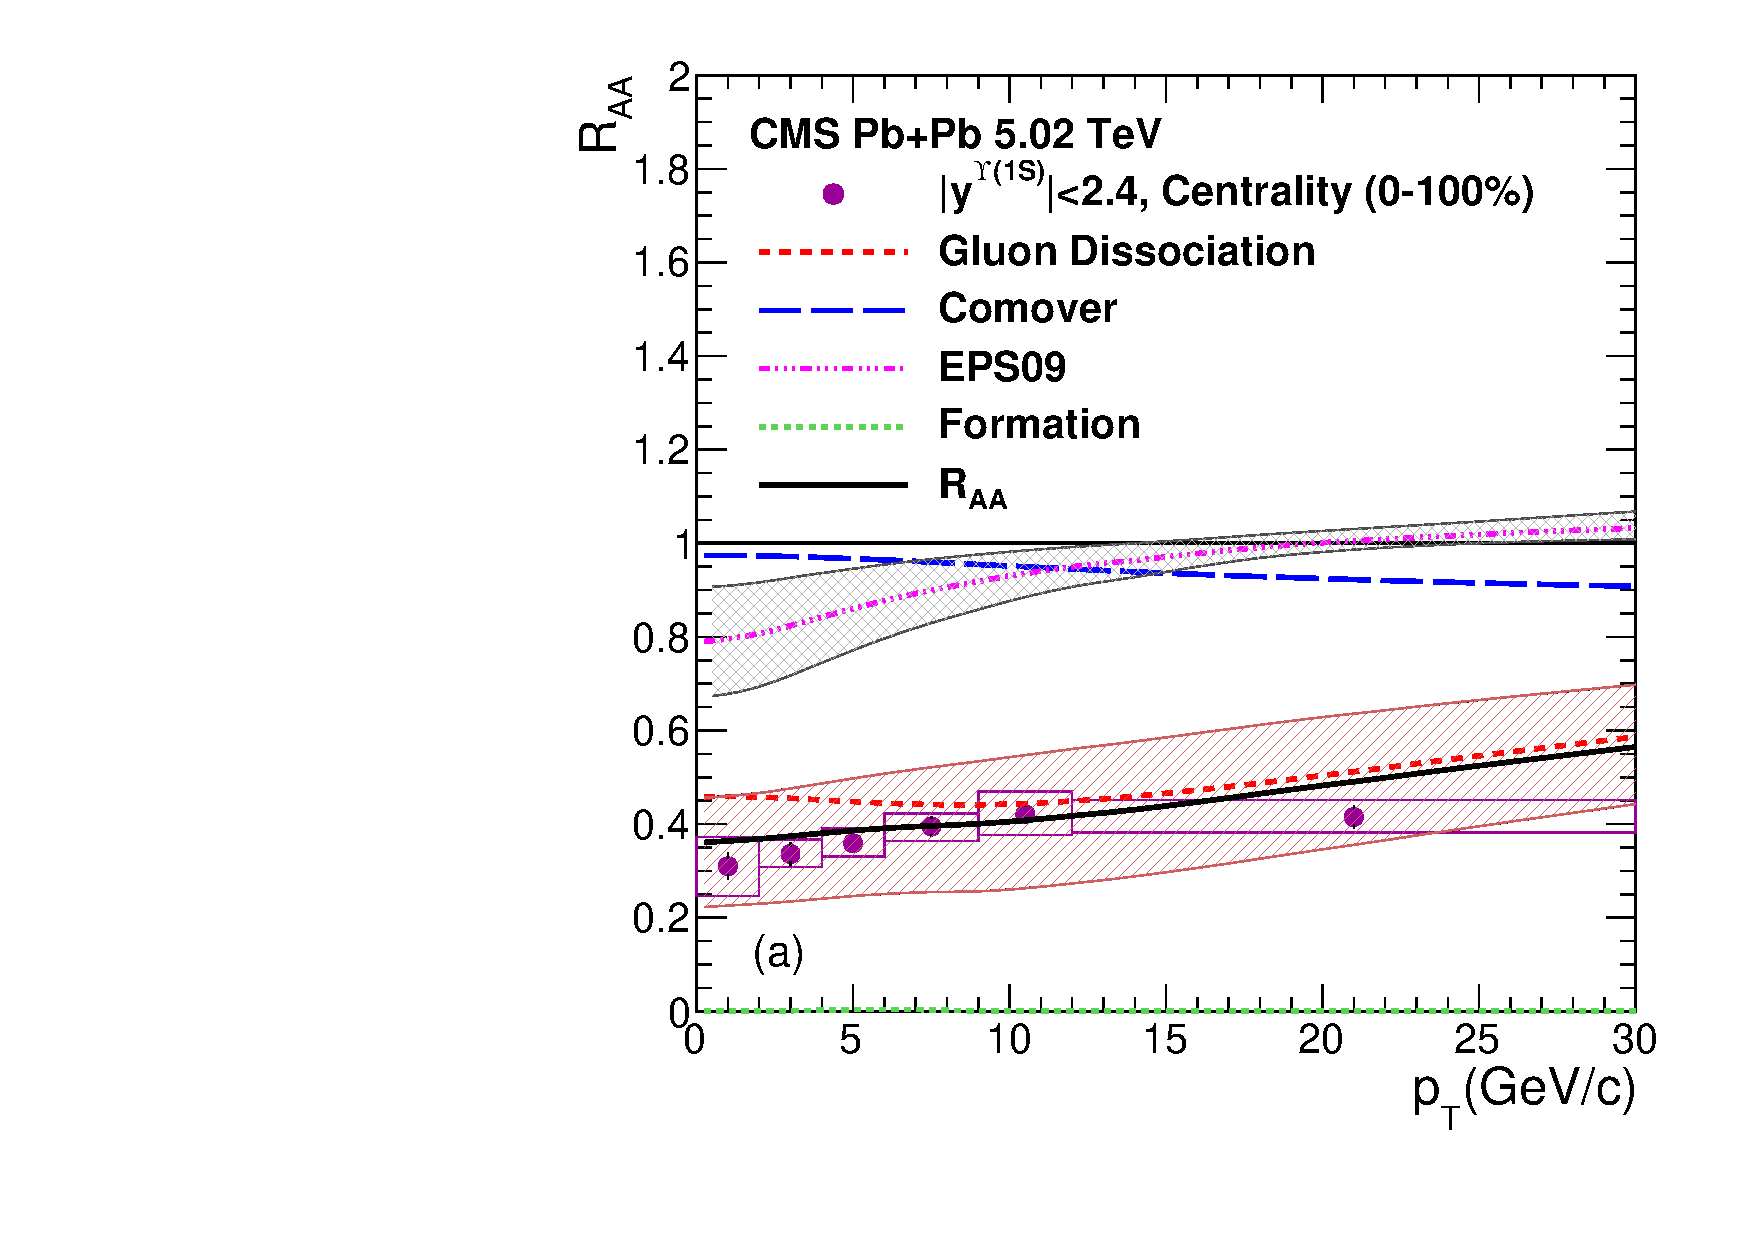
\includegraphics[width=0.49\textwidth]{Figures/Fig20l_Y1S_CMS_RAAPt_Shade.pdf}
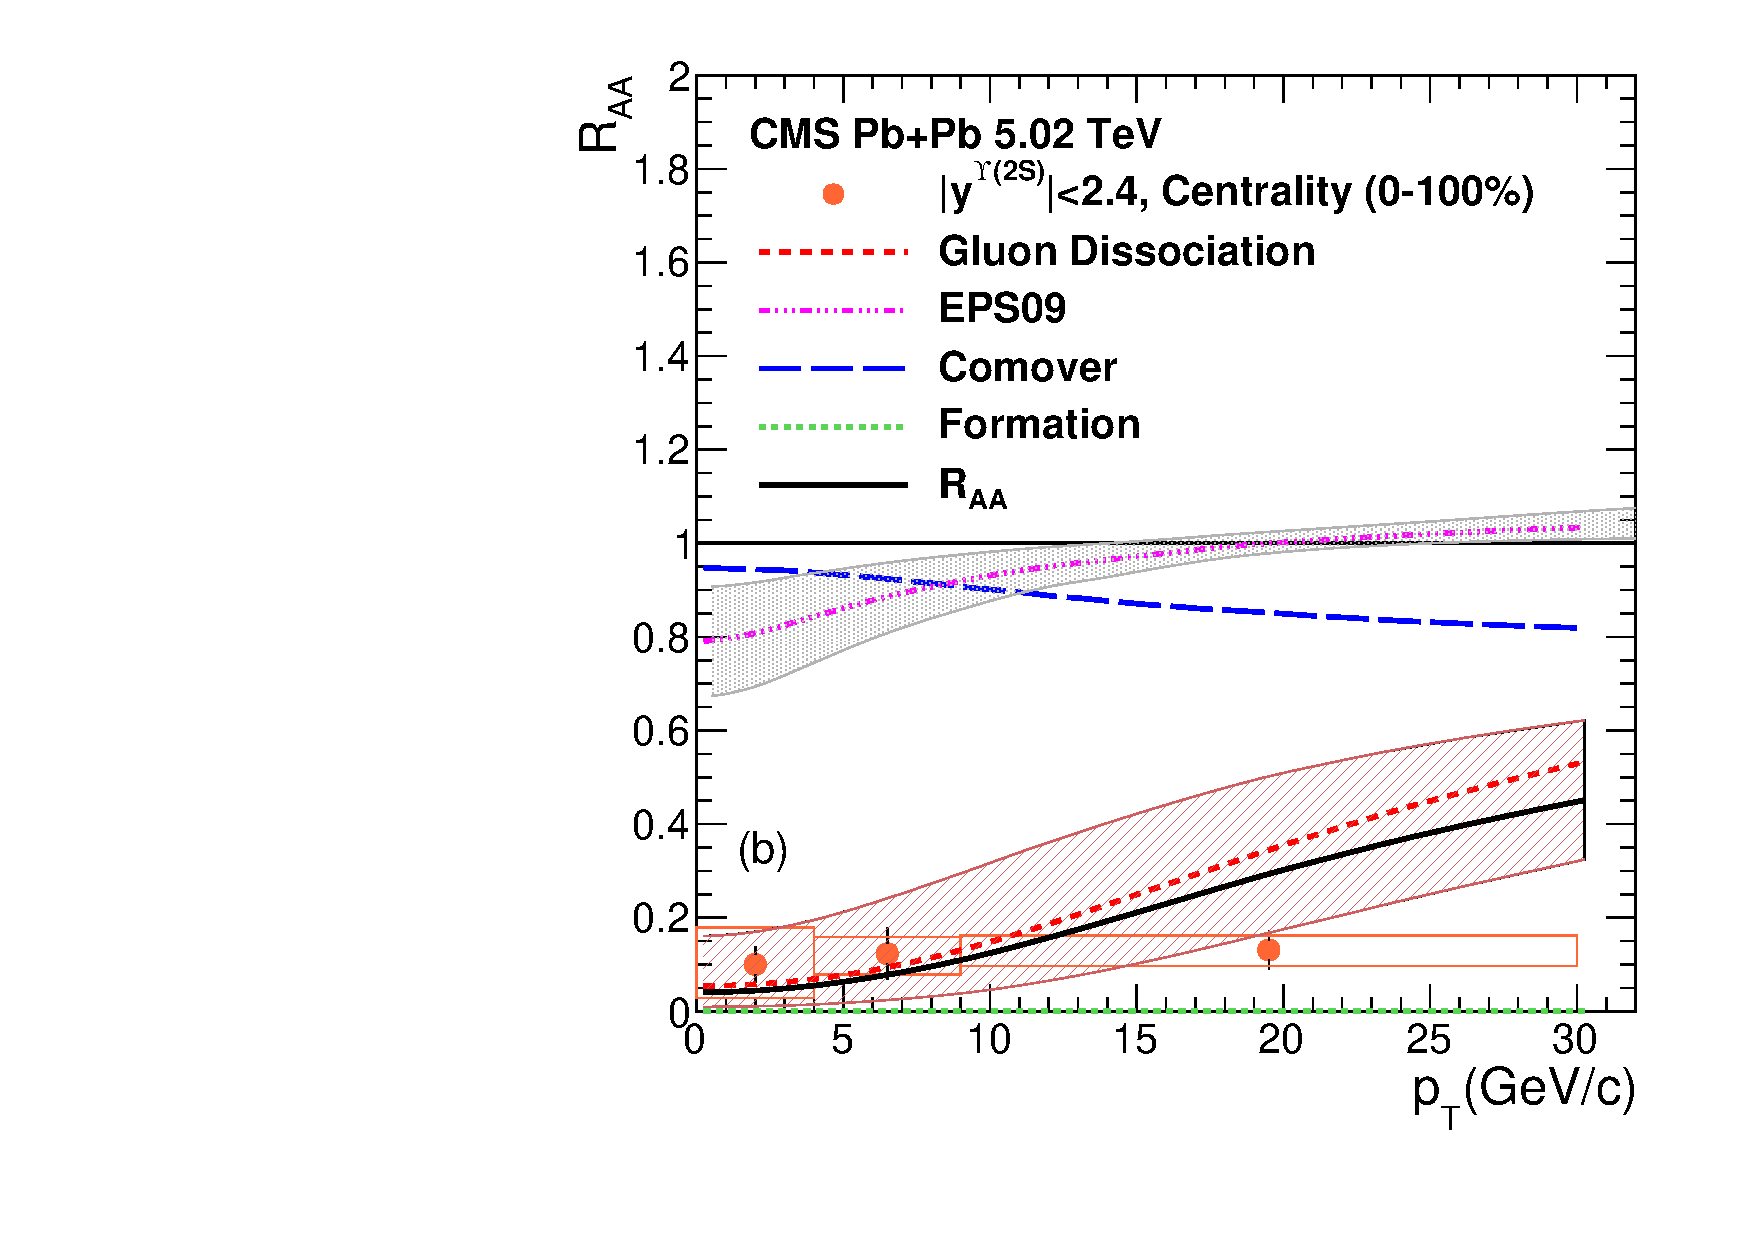
\includegraphics[width=0.49\textwidth]{Figures/Fig20r_Y2S_CMS_RAAPt_Shade.pdf}
\caption{(Color online) Calculated nuclear modification factor ($R_{AA}$) \cite{Kumar:2019xdj}
  of (a) $\Upsilon$(1S) and 
  (b) $\Upsilon$(2S) as a function of $p_{T}$ 
  compared with CMS measurements~\cite{CMS:2018zza}.
The global uncertainty in $R_{AA}$ is shown as a band around the line at 1.
}
\label{fig:UpsilonRaaPtCMS}
\end{figure}



\begin{figure}
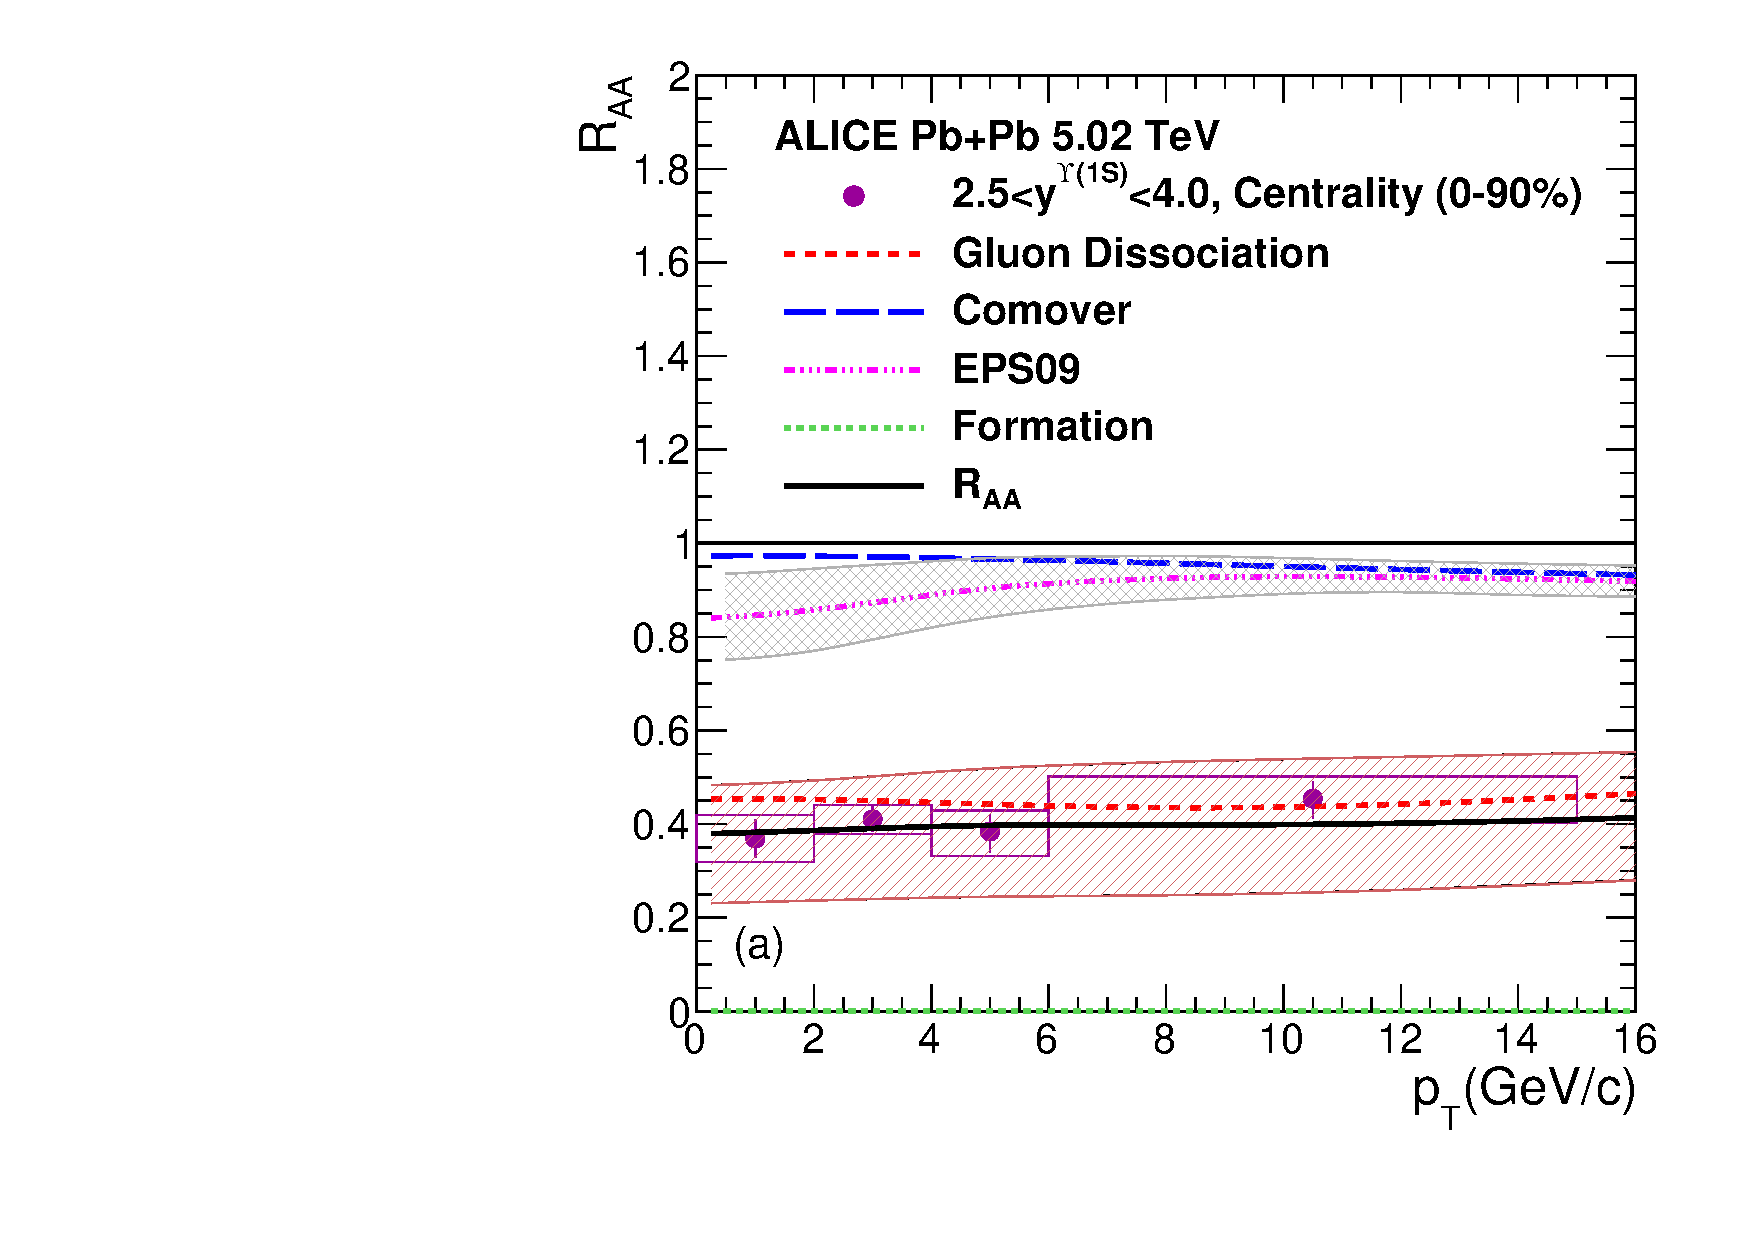
\includegraphics[width=0.49\textwidth]{Figures/Fig21l_ALICE_Y1SRAAPt_Shade.pdf}
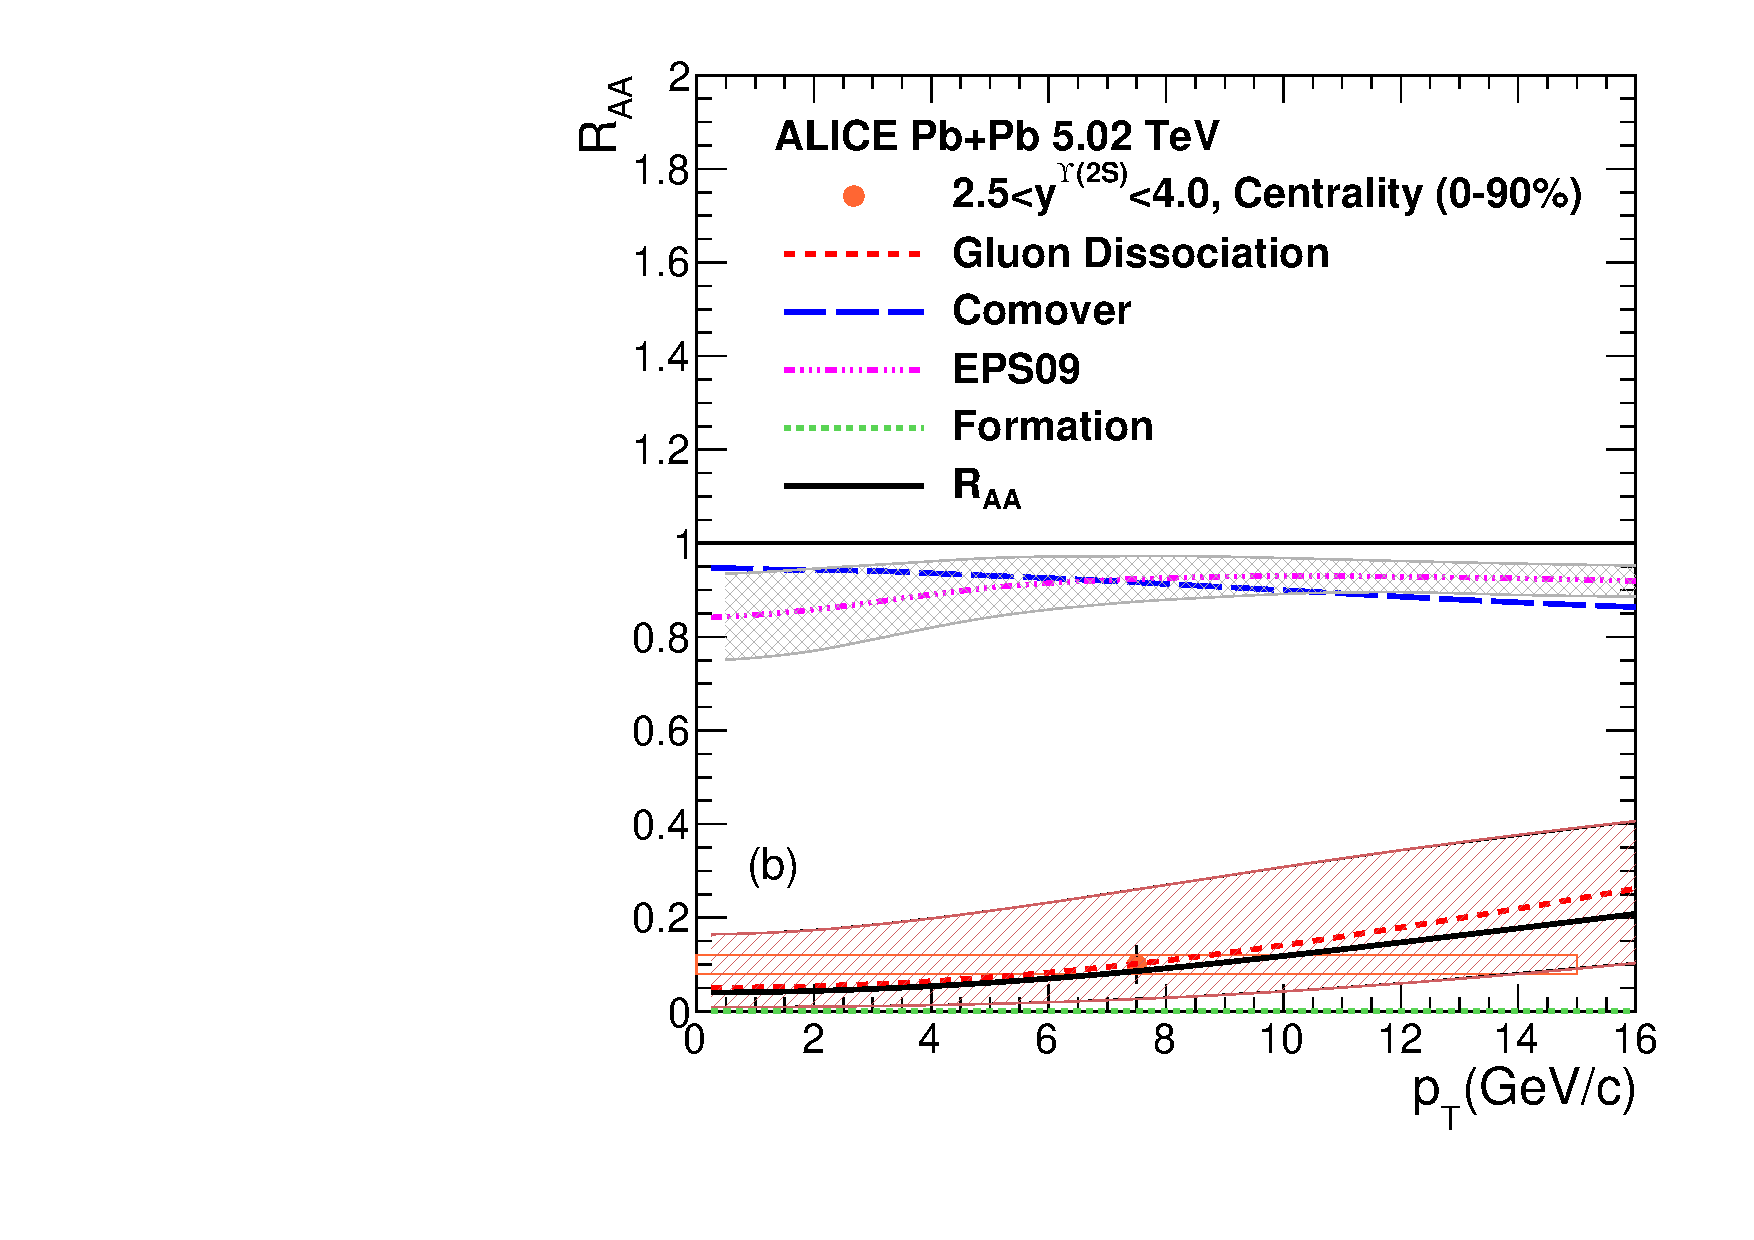
\includegraphics[width=0.49\textwidth]{Figures/Fig21r_ALICE_Y2SRAAPt_Shade.pdf}
\caption{(Color online) Calculated nuclear modification factor ($R_{AA}$) \cite{Kumar:2019xdj}
  of (a) $\Upsilon$(1S) and 
  (b) $\Upsilon$(2S) as a function of $p_{T}$ in the kinematic range of ALICE detector
at LHC ~\cite{ALICE:2020wwx}. The global uncertainty in $R_{AA}$ is shown as a band
around the line at 1.
} 
\label{fig:UpsilonRaaPtALICE}
\end{figure}

\begin{figure}
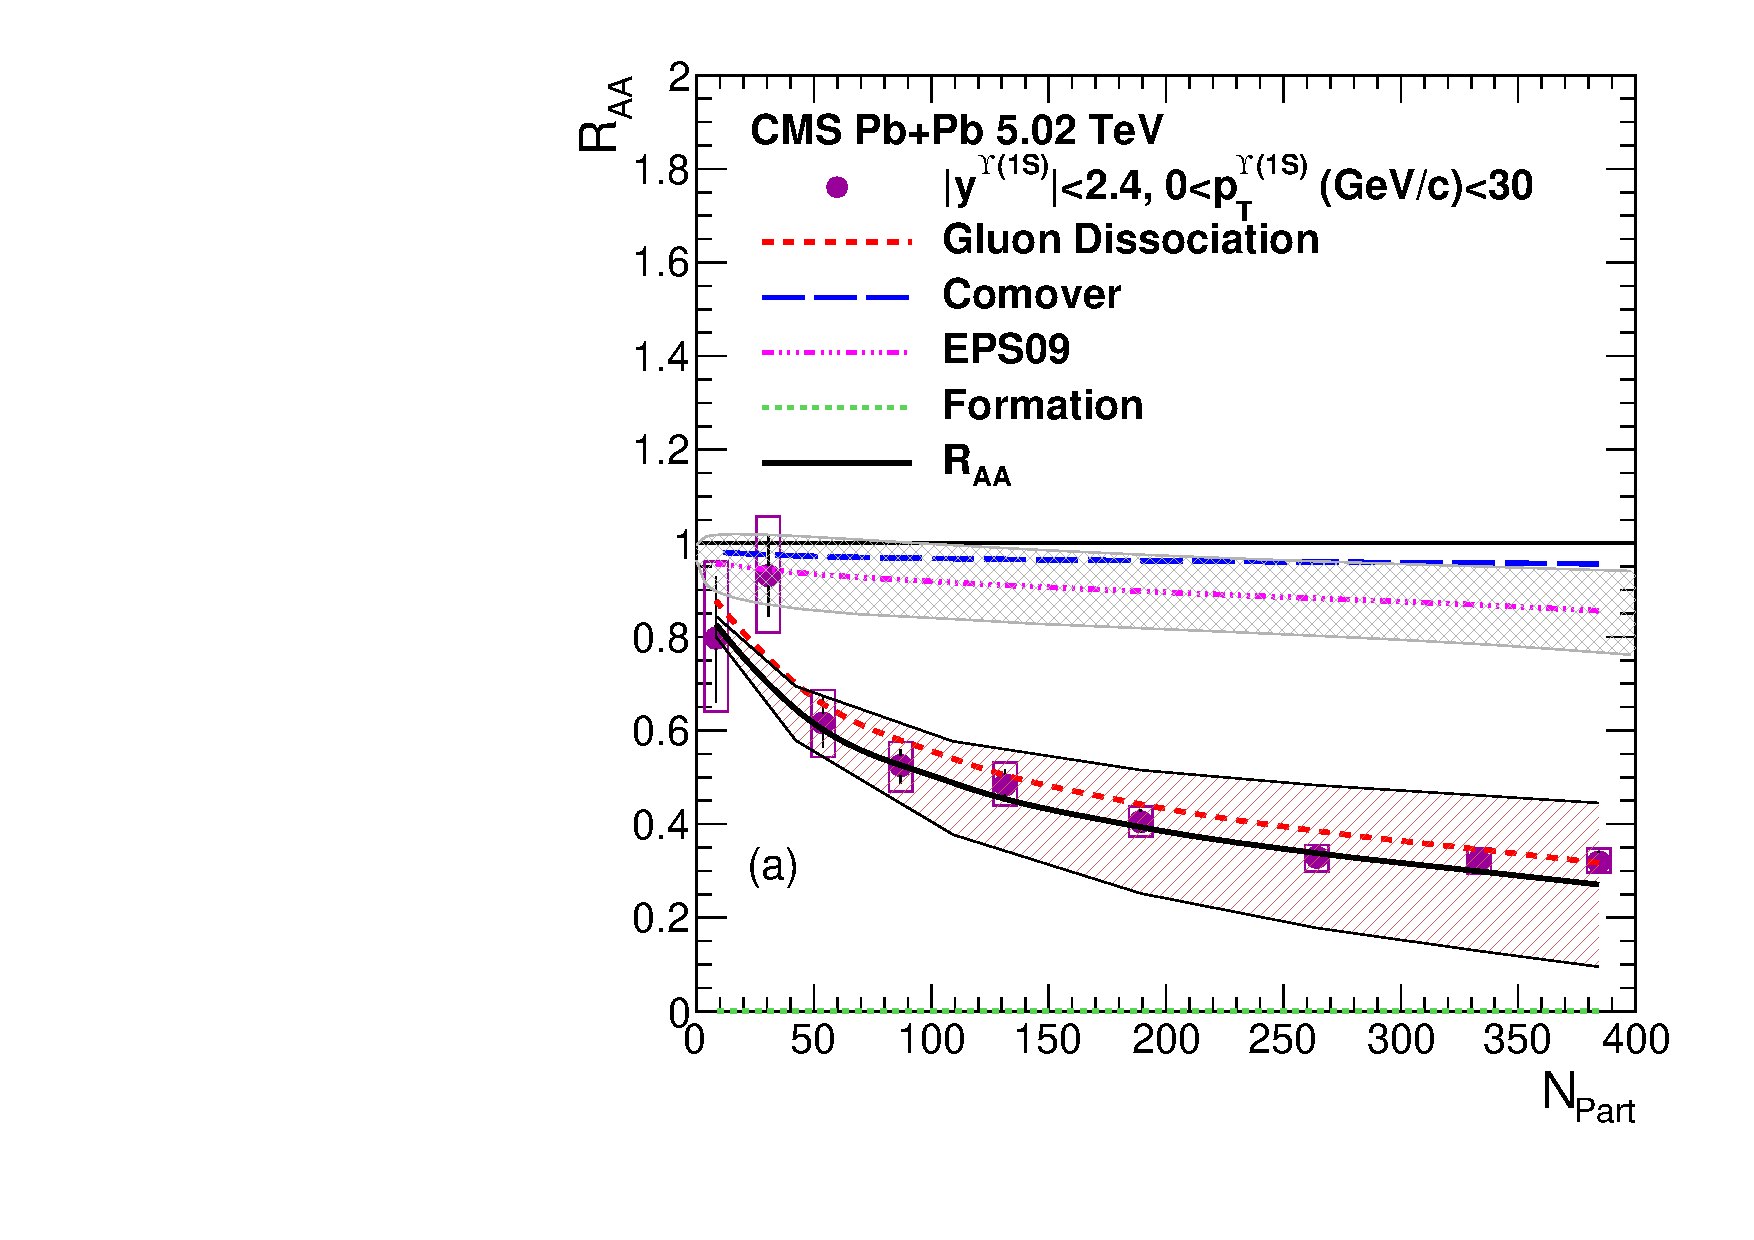
\includegraphics[width=0.49\textwidth]{Figures/Fig22l_CMS_Y1SRAANPart_Shade.pdf}
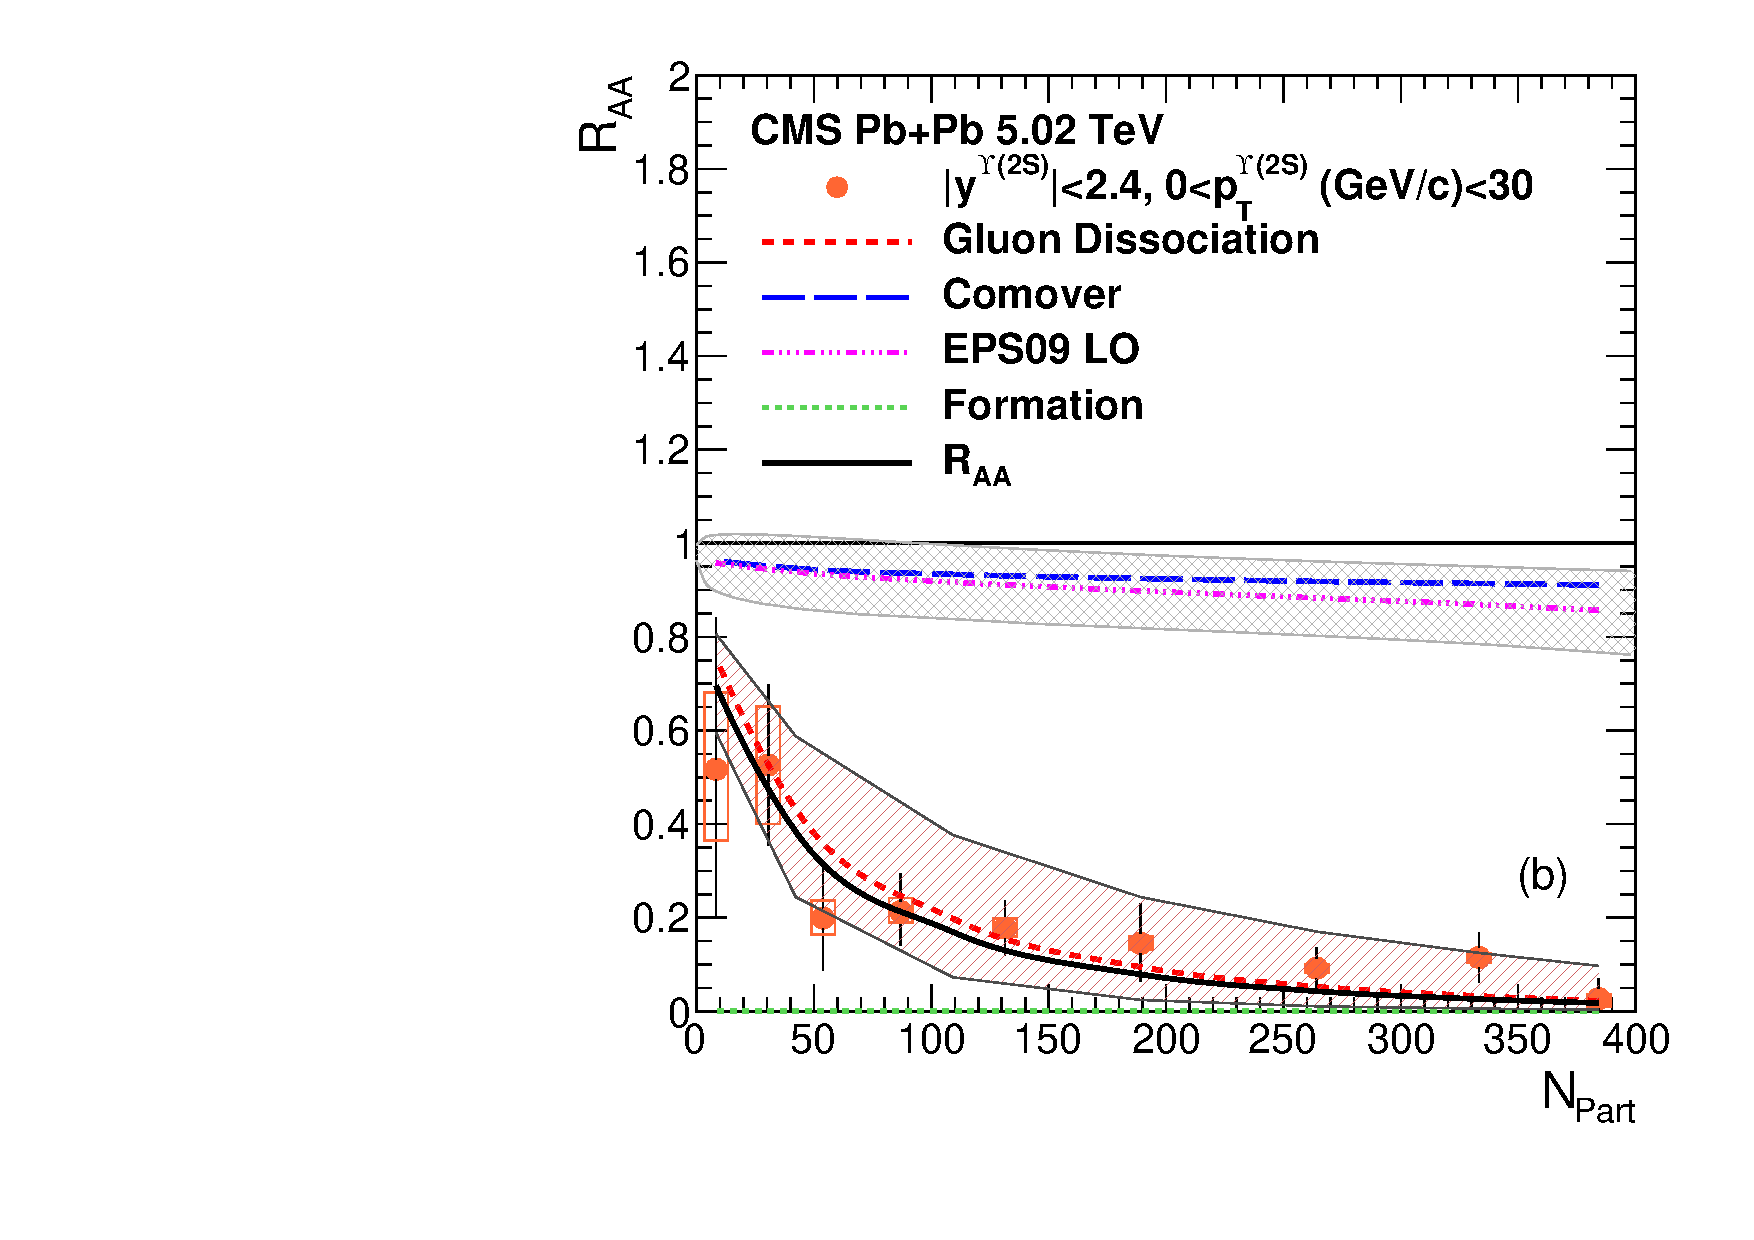
\includegraphics[width=0.49\textwidth]{Figures/Fig22r_CMS_Y2SRAANPart_Shade.pdf}
\caption{(Color online) Calculated nuclear modification factor ($R_{AA}$) \cite{Kumar:2019xdj} of 
  (a) $\Upsilon$(1S) and (b) $\Upsilon$(2S) as a function of centrality of the 
  collisions compared with the CMS measurements~\cite{CMS:2018zza}.%\cite{CMS:2017ucd}.
  The global uncertainty in $R_{AA}$ is shown as a band around the line at 1.
}
\label{fig:UpsilonRaaNPartCMS}
\end{figure}


Figure~\ref{fig:UpsilonRaaPtCMS}(a) and (b) show the calculations~\cite{Kumar:2019xdj}
of various contributions to
the nuclear modification factor, $R_{AA}$, for the $\Upsilon$(1S) and $\Upsilon$(2S)
respectively as a function of $p_T$ compared with the mid rapidity measurements from
CMS~\cite{CMS:2018zza}.  
The gluon dissociation mechanism combined with the pion dissociation and shadowing
corrections gives good description of data in $p_{T}$ range ($p_{T}\approx$ 0-15 GeV/c)
for both $\Upsilon$(1S) and $\Upsilon$(2S).
The contribution from the regenerated $\Upsilon$s is negligible even at LHC energies.
The calculations under-predict the suppression observed at the highest measured
$p_{T}$ for $\Upsilon$(1S) and $\Upsilon$(2S) which is similar for the case
of J/$\psi$.
%The feed-down corrections are applied in our calculations following the similar
%procedure as in Refs.~\cite{Abdulsalam:2012bw,Krouppa:2017jlg}. 
%%%%%%%%% insert the feed-down details here

The feeddown corrections in the states $\Upsilon$(1S) and $\Upsilon$(2S) 
from decays of higher b$\bar{\rm b}$ bound states are obtained as
  \begin{equation}
    R_{AA}^{\Upsilon(3S)} = R_{AA}^{\Upsilon(3S)}, %\nonumber
  \end{equation}
  \begin{equation}
    R_{AA}^{\Upsilon(2S)} = f_1 R_{AA}^{\Upsilon(2S)} +  f_2 R_{AA}^{\Upsilon(3S)},  %\nonumber
  \end{equation}
   \begin{equation}
    R_{AA}^{\Upsilon(1S)} = g_1 R_{AA}^{\Upsilon(1S)} +  g_2 R_{AA}^{\chi_b(1P)} + g_3 R_{AA}^{\Upsilon(2S)} + g_4 R_{AA}^{\Upsilon(3S)}. %\nonumber
  \end{equation}
The factors $f$'s and $g$'s are obtained from CDF measurement~\cite{Affolder:1999wm}.
The values of $g_1$, $g_2$, $g_3$ and $g_4$ are 0.509, 0.27, 0.107
and 0.113 respectively. Here $g_4$ is assumed to be the combined fraction of 
$\Upsilon$(3S) and $\chi_b$(2P).
The values of $f_1$ and $f_2$ are taken as 0.50~\cite{Strickland:2011aa}.


Figure~\ref{fig:UpsilonRaaPtALICE}(a) and (b) show the model 
prediction \cite{Kumar:2019xdj} of the nuclear modification factor, $R_{AA}$, for the $\Upsilon$(1S)
and $\Upsilon$(2S) respectively as a function of $p_T$ in the kinematic range
covered by ALICE detector. The ALICE data~\cite{ALICE:2020wwx} is well described by the model.

Figure~\ref{fig:UpsilonRaaNPartCMS}(a) depicts the calculated \cite{Kumar:2019xdj}
centrality dependence of the $\Upsilon$(1S) nuclear
modification factor, along with the midrapidity data from CMS~\cite{CMS:2018zza}.
The calculations combined with the pion dissociation and shadowing corrections 
gives very good description of the measured data. Figure~\ref{fig:UpsilonRaaNPartCMS}(b)
shows the same for the $\Upsilon$(2S) along with the midrapidity
CMS measurements. The suppression of the excited $\Upsilon$(2S) states 
is also well described by the model. As stated earlier, the effect of regeneration is
negligible for $\Upsilon$ states. 

To summarise, the gluon dissociation mechanism combined with the shadowing
corrections gives very good description of data in mid $p_{T}$ range ($p_{T}\approx$ 5-10 GeV/c)
for both $\Upsilon$(1S) and $\Upsilon$(2S).
The contribution from the regenerated $\Upsilon$s is negligible even at LHC energies.
The calculations under-predict the suppression observed at the highest measured
$p_{T}$ for $\Upsilon$(1S) and $\Upsilon$(2S) which is similar for the case
of J/$\psi$.


  The suppression of quarkonia by comoving pions can be calculated by folding the quarkonium-pion
dissociation cross section $\sigma_{\pi Q}$ over thermal pion distributions \cite{Vogt:1988fj}. 
It is expected  that at LHC energies, the comover cross section will be small~\cite{Lourenco:2008sk}.
{\color{black}
The pion-quarkonia cross section is calculated by convoluting the gluon-quarkonia cross section $\sigma_D$
over the gluon distribution inside the pion~\cite{Arleo:2001mp},
\begin{equation}
\sigma_{\pi Q} (p_{\pi}) = {p_+^2 \over 2(p_\pi^2 - m_\pi^2)} \int_0^1 \, dx \, G(x) \, \sigma_D(xp_+/\sqrt {2}),
\end{equation}
where $p_+ = (p_\pi + \sqrt{p_\pi^2-m_\pi^2})/\sqrt{2}$. The gluon distribution, $G(x)$, inside a pion is 
given by the GRV parameterization~\cite{Gluck:1991ey}. 
The dissociation rate $\lambda_{D_{\pi}}$  can be obtained using the 
thermal pion distribution.




\subsection{Transport approach for bottomonia in the medium}
 The studies in Refs.~\cite{Grandchamp:2005yw,Rapp:2017chc} use 
transport approach for the bottomomia production in the medium~\cite{Grandchamp:2005yw,Rapp:2017chc}.
The rate equation for bottomonium evolution in the medium's rest frame
can be written as,
\begin{equation}
\frac{\mathrm{d} N_Y(\tau)}{\mathrm{d}\tau} =
-\Gamma_Y(T)\left[N_Y(\tau)-N^{\rm eq}_Y(T)\right] \ .
\end{equation}
Here $\Gamma_Y$, is the inelastic reaction rate  and $N^{\rm eq}_Y(T)$ is the thermal
equilibrium limit  for each state $Y=\Upsilon(1S), \Upsilon(2S), \chi_c$.
In the reaction rates  both gluo-dissociation and quasi-free mechanisms have
been incorporated.  An important ingredient in this calculation is the bottomonium
binding energies. The thermal-equilibrium limit is evaluated from the statistical
model with bottom quarks~\cite{Grandchamp:2002wp}. 
The initial conditions are obtained from the p+p collision data. With these inputs,
the study is carried out in a hydrodynamicaly 
expanding scenario.  




\begin{figure}[t]
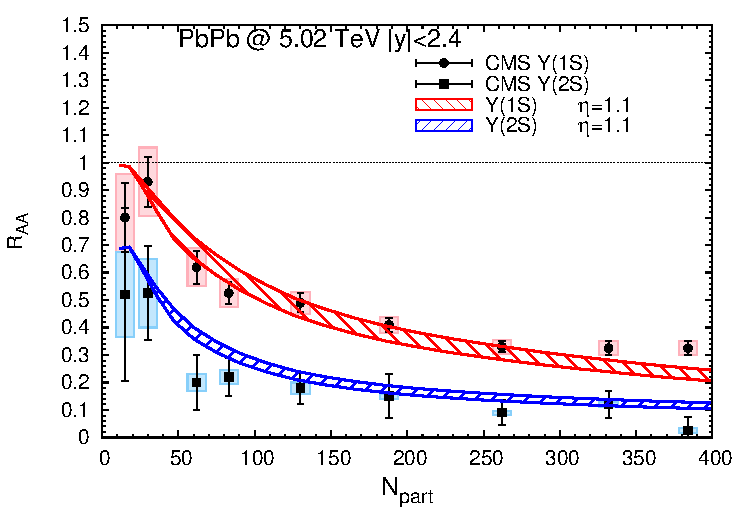
\includegraphics[width=0.49\textwidth]{Figures/Fig23l_YnsRAA_NPart_RappModel.pdf}
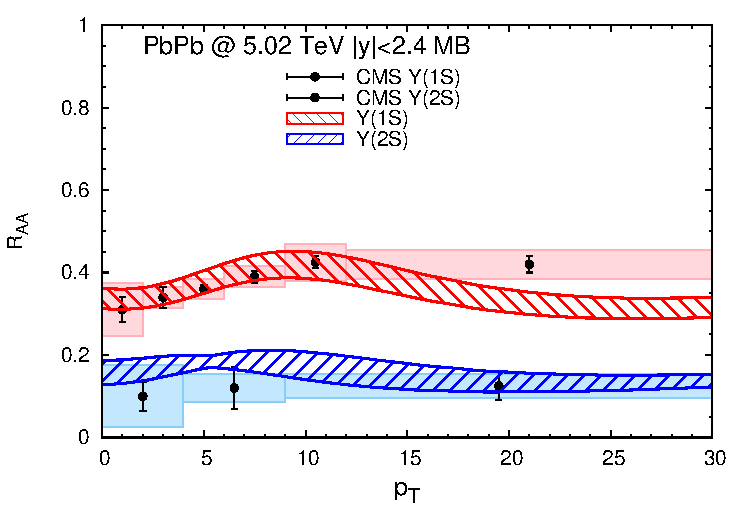
\includegraphics[width=0.49\textwidth]{Figures/Fig23r_YnsRAA_Pt_RappModel.pdf}
\caption{(Color online) Centrality (left) and transverse-momentum (right) dependence of the $R_{\rm AA}$~\cite{Rapp:2017chc}
  for $\Upsilon(1S)$ and $\Upsilon(2S)$ in 5.02\,TeV Pb-Pb collisions at the LHC,
  compared to CMS data~\cite{Flores:2017qmcms}.
  The bands represent a 0-15\,\% shadowing~\cite{Eskola:2009uj} on open-bottom and bottomonia.}
\label{fig_cms}
\end{figure}

Figure \ref{fig_cms} shows the Centrality (left) and transverse-momentum (right)
dependence of the $R_{\rm AA}$ calculated by model in Ref~\cite{Rapp:2017chc}
for $\Upsilon(1S)$ and $\Upsilon(2S)$ in 5.02\,TeV Pb-Pb collisions at the LHC,
compared to CMS data~\cite{Flores:2017qmcms}.
The authors of this model found a reasonable agreement  with experimental data
for the centrality dependence of both $\Upsilon(1S)$ and $\Upsilon(2S)$ at both
collision energies.
%Interestingly, they could reproduce the strong suppression of
%the $\Upsilon(2S)$ observed by STAR.  
%The calculated $p_T$ spectra at 5.02\,TeV appear to capture the rather flat
%shapes in the CMS data at high $p_T$. 






\section{Summary and Conclusions}
\label{sec:conclusions}

In this writeup, we have reviewed the field of bottomonia production in
p+p, p+A and A+A collisions. With immense experimental and theoretical activities
specially due to LHC measurements, many features of the bottomonia production
and their behavior in the medium are well understood.

In section~\ref{Sec:BottPP}, we have reviewed the experimental status of the bottomonia production
in p+p collisions. The measurements at Tevatron, by CDF and D0 collaborations,
have been discussed. The measurements at LHC, by CMS and ATLAS, at ${\sqrt s}=$ 7 TeV and
13 TeV have been reviewed. There have been some measurements 
of $\Upsilon$ polarization by CDF collaboration.
The CMS and LHCb data, on $\Upsilon$ polarizability, confirms 
negligible polarization. 
The measurements of the cross sections and polarizations have shed light on the
$\Upsilon$(1S, 2S, 3S) production mechanisms in p+p collisions.
LHC data has substantially extended the reach of the kinematics to test the
Non-Relativistic QCD (NRQCD) and other models with higher-order corrections which become more
distinguishable at higher transverse momenta.

In section~\ref{sec:Bottomonia_pp_th}, we have discussed theoretical models of the bottomonia production
mechanism in p+p collisions. The bottomonia study in p+p involves heavy quark
pair production treatable by perturbative process and the formation of bottomonia 
which is a non-perturbative process.
For the later one has to take recourse to some effective models. We have discussed the 
color singlet model, the color evaporation model and the NRQCD factorisation approach.
In the color singlet model, it is assumed that the $Q\bar Q$ pair that evolves into
the quarkonium is in a color-singlet state. 
On the other hand in the color evaporation model,
it is assumed that every produced $\QQbar$ pair can evolve into a quarkonium,
if it has an invariant mass that is less than the threshold for
producing a pair of open-flavor heavy mesons.
The probability factor of a pair evolving into quarkonium is obtained by fitting with
the experiments which is supposed to be independent of collision energy. 
The Improved CEM reproduces the transverse momentum dependence of the
quarkonium cross section at CDF and LHC energies.  
We also presented NRQCD model formalism in detail.
The NRQCD formalism, along with the color singlet state, includes the color octet state.
In this formalism the evolution probability of $Q\bar{Q}$
pair into a state of quarkonium is expressed as matrix elements of NRQCD operators
expanded in terms of heavy quark velocity $v$.
The work using NLO cross sections are discussed and LO calculations have been
reproduced for $\Upsilon$(nS) production in p+p collision at $\sqrt s = 7$ and 13 TeV.

In section~\ref{Sec:BottAAexp}, we have presented an experimental overview of the bottomonia
results in p+A and A+A collisions at RHIC and LHC. We have looked into the
$R_{AA}$ for $\Upsilon$(nS) as a function of kinematic variables 
$p_{\rm T}$, rapidity and $N_{\rm Part}$ at different energies and by different experiments. 
We have also studied $v_2$ for these states with centrality and $p_{\rm T}$.
LHC has provided high statistics measurements of $R_{AA}$ for
Pb+Pb collisions for all three Upsilon states over wide kinematical ranges.
All $\Upsilon$ states are found to be suppressed in the Pb+Pb collisions,
the heavier states are more suppressed relative to the ground state.
The suppression of $\Upsilon$ states strongly depends on system size but
has a weak dependence on $\pT$ and rapidity. At high $p_T$, more precise
measurements are required to ascertain flatness in the suppression. 
Comparing the measurements at RHIC and at two energies of LHC, it can be
said that the suppression increases with energy albeit weakly.

All three Upsilon states are suppressed in p+Pb collisions as well
and the excited states are more suppressed than the ground state indicating
final state effects.
We have obtained a new figure for the ratio $\Upsilon$(2S)/$\Upsilon$(1S)
as a function of event activity measured in p+Pb and Pb+Pb collisions at
$\sqrt{s_{\rm NN}}$=5.02 TeV compared with the 
p+p collisions at $\sqrt{s}$=7 TeV. This study shows 
that the ratio $\Upsilon$(2S)/$\Upsilon$(1S) decreases steadily
with with increasing $N_{\rm tracks}$ for
p+p and p+Pb systems and the peripheral Pb+Pb data also follow this trend.
Then there is a step and most central Pb+Pb
data show a flatness as a function of event activity contrary to p+p and
p+Pb collisions which fall steadily with increasing $N_{\rm tracks}$.
This behavior can be used to distinguish the Pb+Pb collision
system with from smaller systems.
 
No significant $v_2$ is found for $\Upsilon$(1S) measured by CMS
experiment. This shows that the bottom quark is not thermalized in the medium.
The recombination yield of bottomonia calculated using our model
is very small. 


In section~\ref{sec:Bottomonia_hi}, we have discussed the mechanisms for the modification of 
bottomonia yields in heavy ion collisions. Starting with the idea of color screening we have
discussed the more recent ideas like the modification of spectral functions of quarkonia states as
a function of temperature.
The cold nuclear matter has been reviewed in a certain amount of detail.
The excited bottomonia states are more suppressed as compared to the ground state,
an effect that can not be understood by the shadowing of NPDFs alone. The final state
effects in p+A collisions require a better theoretical understanding. 
We have reviewed some if not all the theoretical models treating both
the quarkonia dissociation and recombination in the dynamical medium.
The comparison of the theoretical results with the experiments shows that
the bottomonia production can be understood in terms of color screening
or gluon dissociation. There is no significant recombination needed,
a picture that is also consistent with the small values of $v_2$ measured
by the experiments.

 




%\section*{References}
%\printbibliography %% for biber
\bibliography{Bott1Review.bib}


\end{document}


